
\documentclass[a4paper,10pt,fleqn]{article} % Definiert Papier = A4;
                                            % Schriftgrösse = 10Punkte;
                                            % Mathe.-Gl. Modus = linksbündig
                                            % (siehe http://lefti.amigager.de/latex/Aufbau.html)

\usepackage[utf8x]{inputenc}                % utf8x kann alle Textcodierungen interpretieren
\usepackage[T1]{fontenc} %Schriftcodierung mit UTF-8
\usepackage{textcomp} %Erweiterung von fontenc
\usepackage{lmodern} %Erweiterung des Zeichensatzes

\usepackage{graphics}                       % Package für Einfügen/Anpassen von Grafiken
\usepackage{graphicx}
\usepackage{wrapfig}                        % Package zum Einfügen von Textumflossenen Bilder

\usepackage[english,ngerman]{babel}         % ngerman = Neues Deutsch; babel = internationalisierung einschalten
\usepackage[babel,german=quotes]{csquotes}  % Deutsche Gänsefüssechen

\usepackage{hyperref}

\usepackage{amsmath}                        
\usepackage[all]{xy}
%\usepackage[xindy]{glossaries}
\usepackage{makeidx}
\usepackage{pdfpages}
\usepackage{graphicx}
\usepackage{printlen}

\usepackage{blindtext}
\usepackage{lipsum}

\usepackage{multicol}

\usepackage{multirow}

\usepackage{verbatim}

\usepackage{color}

\usepackage{eurosym}

%\usepackage{hyperref}
\usepackage{acronym}

\usepackage{enumitem}

\usepackage{setspace}

\usepackage{threeparttable} %benötigt um Fussnoten in einer Tabelle zu machen
\usepackage{longtable}


\usepackage{spreadtab} %benötigt um in Tabellen zu rechnen
\usepackage{numprint}

%Package damit eine Seite quer genommen werden kann
\usepackage{lscape}

%Damit man eine Zelle farbig markiert werden
\usepackage{colortbl}


%
% Rechnen in Tabellen. Zeichen für den Dezimalpunkt
%
\STsetdecimalsep{{.}}

\definecolor{darkgreen}{rgb}{0,0.6,0}
\usepackage{listings}
\lstset{language=[LaTeX]TeX}
\lstloadlanguages{TeX}
\lstset{basicstyle=\ttfamily\footnotesize,
        numbers=left,
        numberstyle=\tiny,
        numbersep=5pt,
        breaklines=true,
        texcsstyle=\color{black},
        backgroundcolor=\color{gray!10},
        %commentstyle=\color{darkgreen},
        %keywordstyle=\color{red}\bfseries,
        %stringstyle=\color{blue}\bfseries,
        frame=single,
        tabsize=2,
        rulecolor=\color{black!30},
        title=\lstname,
        escapeinside={\%*}{*)},
        breaklines=true,
        breakatwhitespace=true,
        framextopmargin=2pt,
        framexbottommargin=2pt,
        inputencoding=utf8x,
        extendedchars=true,
        literate={Ö}{{\"O}}1
                 {Ä}{{\"A}}1
                 {Ü}{{\"U}}1
                 {ü}{{\"u}}1
                 {ä}{{\"a}}1
                 {ö}{{\"o}}1 
       }
%
% hypersetup etwas genauer
%
\hypersetup{pdftex=true,
            hyperfigures=true,
            hyperindex=true,
            bookmarks=true,
            bookmarksopen=true,
            bookmarksnumbered=true,
            %pdfborder={0 0 0},
            hypertexnames=true,
            colorlinks=true,
            pagebackref=false,
            linktocpage=false,% link "`behing"'
            plainpages=false,
            linkcolor=black,%blue,
            %anchorcolor=black,% Color for anchor text.
            citecolor=black,%green,%Color for bibliographical citations in text.
            filecolor=black,%magenta,%Color for URLs which open local files.
            menucolor=black,%red,%Color for Acrobat menu items. pagecolor color red Color for links to other pages, but currently unused
            urlcolor=black,%red,
            pdfstartview=Fit,
            pdfview={XYZ null null null},
            pdfpagelabels,
            pageanchor=true,
            hypertexnames=false
           }
%
% hypersetup etwas rudimentärer
%
%{
    %colorlinks,
    %citecolor=black,
    %filecolor=black,
    %linkcolor=black,
    %urlcolor=black
%}

\usepackage{url}

\usepackage{cite}
\usepackage{apacite}

\usepackage{pdfpages}                        % Packet für PDF Dateimanipulation laden

\usepackage{fancyhdr}                        % http://en.wikibooks.org/wiki/LaTeX/Page_Layout#Customising_with_fancyhdr

\usepackage{siunitx}                         % benötigt um Tabellen nach einem . auszurichten


\bibliographystyle{apacite}


\pagestyle{fancy} %eigener Seitenstil
\fancyhf{} %alle Kopf- und Fusszeilenfelder bereinigen

\addtolength{\textwidth}{1.5cm}
\addtolength{\evensidemargin}{-5mm}
\addtolength{\oddsidemargin}{-5mm}

\addtolength{\headwidth}{1.5cm}

%\rhead{\setlength{\unitlength}{1mm}
%\begin{picture}(-2,7)
%    \includegraphics[width=35mm]{hslu_logo2.PNG}
%\end{picture}}

\fancyhead[L]{Projektarbeit: Autonomer Ballwerfer} %Kopfzeile links
\fancyhead[C]{} %zentrierte Kopfzeile
\fancyhead[R]{HSLU - T\&A}
%\fancyhead[R]{\includegraphics[scale=0.25]{hslu_logo2.PNG}}
\renewcommand{\headrulewidth}{0.4pt} % obere Trennlinie
\fancyfoot[L]{PREN Team 32}
\fancyfoot[C]{HS - 2014}
\fancyfoot[R]{\thepage}
\renewcommand{\footrulewidth}{0.4pt} % untere Trennlinie

%
% Anpassung der Darstellung des Literaturverzeichnis
%
\let\oldbibliography\thebibliography
\renewcommand{\thebibliography}[1]{%
  \oldbibliography{#1}%
  \setlength{\itemsep}{10pt}%
}
%
% Abbildungen und Tabellen nur mit Kurzform angeben
%
\addto\captionsngerman{
\renewcommand{\figurename}{Abb.}
\renewcommand{\tablename}{Tab.}
}
%
% Benötigt um von zwei Stellen im Text auf dieselbe Fusszeile zu referenzieren
%
\newcommand{\footnoteremember}[2]{%
  \footnote{#2\label{#1}}
  \newcounter{#1}
  \setcounter{#1}{\value{footnote}}
}
\newcommand{\footnoterecall}[1]{%
  \hyperref[#1]{\footnotemark[\value{#1}]}
} 
\makeatletter
\providecommand{\rowno}[1][__empty__]
{%
  \ifthenelse{\isundefined{\c@rowno}}
  {%
    \newcounter{rowno}
  }
  {}%
  	\ifthenelse{\equal{#1}{__empty__}}
 	 {%
       \stepcounter{rowno}%
     }
     {%
 	   \setcounter{rowno}{#1}%
     }%
  \therowno%
}
\makeatother
%
%\makeglossaries
%\include{wa/wa_glossar}
%
%\documentclass[a4paper,10pt,fleqn]{article} % Definiert Papier = A4;
%                                            % Schriftgrösse = 10Punkte;
%                                            % Mathe.-Gl. Modus = linksbündig
%                                            % (siehe http://lefti.amigager.de/latex/Aufbau.html)
%
%\usepackage{Common/Layout}
\newcommand{\BrushlessPath}{Enddokumentation/ET_Gruppe}
\newboolean{STANDALONE}
\setboolean{STANDALONE}{false}

\newboolean{EMBED}
\setboolean{EMBED}{false}

\setboolean{EMBED}{true}
\newcommand{\myTitel}{Dokumentation}
\newcommand{\BLDCTeams}{T27 und T32}
\newcommand{\BLDCcollab}{Dieses Kapitel ist eine Zusammenarbeit der Gruppen \BLDCTeams. }
\begin{document}
    %
    % Deck- und Titelblatt
    %
    \begin{titlepage}
    \begin{center}     
        \parindent0pt{\Huge PREN 1}\\
        \vspace*{1.2cm}
        Yves Studer\\
        Thomas Wiss\\
        Livio Kunz\\
        Nikolaus Manser\\
        MatteoTrachsel\\
        Güdel Manuel\\
        Pascal Roth\\
        \vspace*{1.2cm}
        {\Huge \myTitel}\\
        \vspace*{1cm}
%        \begin{figure*}[h!]
%            \centering
%            \includegraphics[width=0.7\textwidth]{Sourcen/Bilder/WuerfelTitel}
%        \end{figure*}
        \vspace*{10cm}
        {\normalsize Hochschule Luzern - Technik \& Architektur}\\
        {\normalsize PREN 1}\\
        \vspace*{0.6cm}
        {\normalsize Horw, Hochschule Luzern - T\&A, \today}\\
    \end{center}
\end{titlepage}

    \begin{titlepage}
    \parindent0pt {\Huge PREN 1}\\
    \vspace*{0.7cm}
    \newline
    \begin{tabular}{ p{6cm} p{5cm}}
        Yves Studer                & Thomas Wiss \\
        Dorfstrasse 28             & Bachhüsliweg 4a \\
        6264 Pfaffnau              & 6042 Dietwil \\
        +41 79 705 48 88           & +41 79 604 93 61 \\
        yves.studer@stud.hslu.ch   & thomas.wiss@stud.hslu.ch \\
                                   & \\
        Livio Kunz                 & Niklaus Manser \\
        Hubelmatt 7                 & Brunnmattstrasse 11\\
        6206 Neuenkirch         & 6010 Kriens \\
        +41 79 811 53 03           & +41 77 405 58 56 \\
        livio.kunz@stud.hslu.ch    & niklaus.manser@stud.hslu.ch \\
                                   & \\
        Matteo Trachsel			   & Manuel Güdel \\
        Hofstrasse 4               & Riedtalstrasse 4\\
        6004 Luzern                & 4800 Zofingen\\
        +41 79 511 57 88           & +41 79 774 41 40 \\
        matteo.trachsel@stud.hslu.ch & manuel.guedel@stud.hslu.ch \\
        						   & \\
        Pascal Roth			       & \\
        Dorfstrasse 18			   & \\
        6275 Ballwil		       & \\
        +41 79 717 68 94	       & \\
        pascal.roth@stud.hslu.ch   & \\
    \end{tabular}
    \vspace*{1.7cm}
    \newline
    {\Huge Meilenstein 1 Dokumentation}\\
    \vspace*{1.2cm}\\
    {\normalsize Dozent: Markus Thalmann}\\
    \vspace*{0.2cm}\\
    {\normalsize Hochschule Luzern - Technik \& Architektur}\\
    {\normalsize Interdisziplinäre Projekarbeit 2014}\\
    \vspace*{2.3cm}
    \newline
    {\normalsize Horw, Hochschule Luzern - T\&A, \today}\\
\end{titlepage}

    %
    % Management Summary
    % 
    \section*{Abstract}

Da wir nicht einer Meinung sind, welches Abstract aussagekräftiger ist, bitte wir Sie um Ihr Feedback.

\subsection{Abstract 1}
<<<<<<< HEAD
Die nachfolgende Dokumentation beschreibt den Konzeptfindungsprozess zur Herstellung eines autonomen Ballwerfers. Die Aufgabe bestand darin, eine Konstruktion zum Werfen von fünf Tennisbällen über eine Kurzdistanz in einen Korb zu entwickeln. Anhand einer Funktionsskizze wurde die Aufgabenstellung in einzelne Teilprobleme zerlegt, zu deren Bewertung ein Morphologischer Kasten gehört.
Zur Bewertung der einzelnen Lösungen dient wiederum das Erstellen von Testmodellen. In einem Feinkonzept wurden weitere Subteilprobleme definiert. Mögliche Lösungen zu diesen stehen in Form eines Auswahlkataloges zur Verfügung. Erarbeitete Berechnungen unterstützen die Bestimmung der Auslegung der einzelnen Komponenten. Als Gesamtlösung kristallisierte sich der Einsatz von zwei Schwungrädern, die durch bürstenlose Motoren angetrieben sind, heraus.
Die Ansteuerung soll mit einem eigens entwickelten Regler erfolgen. Mit einer Smartphone-Kamera wird ein Bild erzeugt, welches anschliessend durch eine eigens entwickelte Applikation ausgewertet und im Zuge dessen die Position des Korbes bestimmt wird. Die selber entwickelten Komponenten Korberkennung und Regelung bieten eine höhere Flexibilität und stellen zugleich einen erhöhten Lerneffekt sicher.
=======
Die nachfolgende Dokumentation beschreibt den Konzeptfindungsprozess zur Herstellung eines autonomen Ballwerfers. Die Aufgabe bestand darin, eine Konstruktion zum Werfen von fünf Tennisbällen über eine Kurzdistanz in einen Korb zu entwickeln. Anhand einer Funktionsskizze wurde die Aufgabenstellung in einzelne Teilprobleme zerlegt, zu deren Bewertung ein Morphologischer Kasten gehört.Zur Bewertung der einzelnen Lösungen dient wiederum das Erstellen von Testmodellen. In einem Feinkonzept wurden weitere Subteilprobleme definiert. Mögliche Lösungen zu diesen stehen in Form eines Auswahlkataloges zur Verfügung. Erarbeitete Berechnungen unterstützen die Bestimmung der Auslegung der einzelnen Komponenten. Als Gesamtlösung kristallisierte sich der Einsatz von zwei Schwungrädern, die durch bürstenlose Motoren angetrieben sind, heraus.Die Ansteuerung soll mit einem eigens entwickelten Regler erfolgen. Mit einer Smartphone-Kamera wird ein Bild erzeugt, welches anschliessend durch eine eigens entwickelte Applikation ausgewertet und im Zuge dessen die Position des Korbes bestimmt wird. Die selber entwickelten Komponenten Korberkennung und Regelung bieten eine höhere Flexibilität und stellen zugleich einen erhöhten Lerneffekt sicher.
>>>>>>> origin/master

\subsubsection{Abstract 2}
In der nachfolgenden Dokumentation wird der Prozess der Konzeptfindung für die Herstellung eines autonomen Ballwerfers beschrieben. Durch die Aufteilung der Aufgabenstellung in Problembereiche werden mehrere unterschiedliche Konzepte geschaffen. Von den erstellten Konzepten wurde eines weiter zu einem Feinkonzept ausgearbeitet, in welchem sämtliche verwendeten Komponenten spezifiziert werden. Als erstes wird das Startsignal von einem Laptop drahtlos via Bluetooth übertragen. Daraufhin lokalisiert der fixstehende Ballwerfer den Korb unter Verwendung einer Smartphonekamera, auf welchem eine entsprechende Applikation zur Korberkennung läuft. Ist die Position einmal bestimmt, wird die Position an den Controller weitergegeben, welcher den Steppermotor für die Ausrichtung des Werfers betätigt und anschliessend die Ballzuführung startet. Der Ballwerfer selbst ist statisch und richtet sich an der Startposition für einen gewinkelten Wurf aus. Einmal ausgerichtet, werden die Bälle einzeln unter Verwendung von Schwungrädern geworfen.

    \addcontentsline{toc}{section}{Abstract}
    \newpage
    %
    % Inhaltsverzeichnis umbenennen und anschliessend einen Seitenumbruch
    % 
    \renewcommand{\contentsname}{Inhalt}
    \tableofcontents
    \newpage
    %
    % Start mit der eigentlichen Arbeit
    %  
    \newpage
    \section{Einleitung}
Im heutigen Arbeitsumfeld ist es unerlässlich, dass man in der Lage ist in einem interdisziplinär zusammengesetzten Team, zu arbeiten. An diesem Punkt setzt die Hochschule Luzern Technik \& Architektur mit dem Modul \enquote{Produktentwicklung} (PREN) an. Das Ziel dieses Moduls ist, anhand einer Aufgabenstellung einen Entwicklungsprozess durch zu arbeiten und in einem interdisziplinären Team eine Lösung zu erarbeiten und umzusetzen. Die Teams bestehen aus Studierenden aus den Studiengängen Elektrotechnik, Informatik und Maschinenbau. Dieses Modul ist in zwei Teile aufgeteilt und erstreckt sich über zwei Semester. Im PREN 1 wird anhand der Aufgabenstellung ein Lösungskonzept entwickelt und erarbeitet. Dieses Konzept wird im anschliessenden Semester im Modul PREN 2 umgesetzt.\\
\\
In diesem Rahmen erhielten die Teams dieses Jahr die Aufgabe, einen autonomen Ballwerfer zu erarbeiten. Das Ziel besteht darin, fünf Tennisbälle, in möglichst kurzer Zeit, in einen Korb zu befördern. Als weiteres Bewertungskriterium gilt das Gewicht des Produkts, welches ab zwei Kilogramm ein stufenweiser Punkteabzug zur Folge hat. Der Korb befindet sich in einem Spielfeld - welches seitlich und in der Höhe begrenzt ist - am hinteren Ende an einer Wand und ist horizontal verschiebbar. Die endgültige Position des Korbes wird kurz vor der Abgabe des Startsignals durch einen Dozenten festgelegt, und ist somit nicht bekannt. Die Übermittlung des Startsignals muss drahtlos erfolgen, nach Ausführen der Aufgabe, muss entweder ein akustisches, oder ein optisches Endsignal ausgegeben werden.\\
\\
Das Ziel der Arbeit ist, die Aufgabenstellung erfolgreich in einem Apparat umzusetzen. Dabei hat sich unser Team eigene Ziele gesetzt und gewichtet. Diese sind:
\begin{enumerate}
    \item Treffgenauigkeit
    \item Geschwindigkeit
    \item Gewicht
\end{enumerate}
%Das Produktentwicklungsmodul ist in zwei Teile aufgeteilt, das PREN1-Modul im Herbstsemester sowie das PREN2-Modul im Frühlingssemester. Wichtigste Aufgabe im PREN1-Modul ist das erarbeiten eines Konzepts, eine professionelle, strukturierte Projektabwicklung und das Verifizieren kritischer Teilprobleme mittels Funktionsmuster. Die Realisation des erarbeiteten Konzepts wird im PREN2-Modul in Angriff genommen.
%    \newpage
%    \section{Zielsetzung}
Im Team wurden die internen Ziele besprochen und wie folgt bestimmt. Die Aufzählung entspricht der Gewichtung:
\begin{enumerate}
\item Treffgenauigkeit
\item Geschwindigkeit
\item Gewicht
\end{enumerate}
Als optionales Ziel wurde beschlossen, dass das Gerät möglichst auch als Tennisballmaschine verwendbar (erweiterbar)
sein soll.\\
\\
\textbf{Weiter wollen wir die höchste Punktzahl erreichen!}

    \newpage
    \section{Von der Recherche zum Feinkonzept}
Um Eckpfeiler für die zu Beginn des Projekts benötigten Recherchen zu erhalten, musste das
Problem grob in seine Teilprobleme zerlegt werden. Aus dieser Zerlegung resultierten die
Bereiche Kommunikation zwischen elektronischen Geräten, Möglichkeiten zur Objekterkennung und
Objektverfolgung, diverse Flugobjekte und Fahrantriebe, Bedarf von Dreh- und Wurfmechanismen
sowie ein Versorgungskonzept. \\
Um Übersicht über die Teilprobleme zu behalten wurde eine Funktionsskizze geschaffen, welche
in  Abbildung \ref{fig:Funktionsskizze} ersichtlich ist.\\
\begin{figure}[h!]
	\centering
	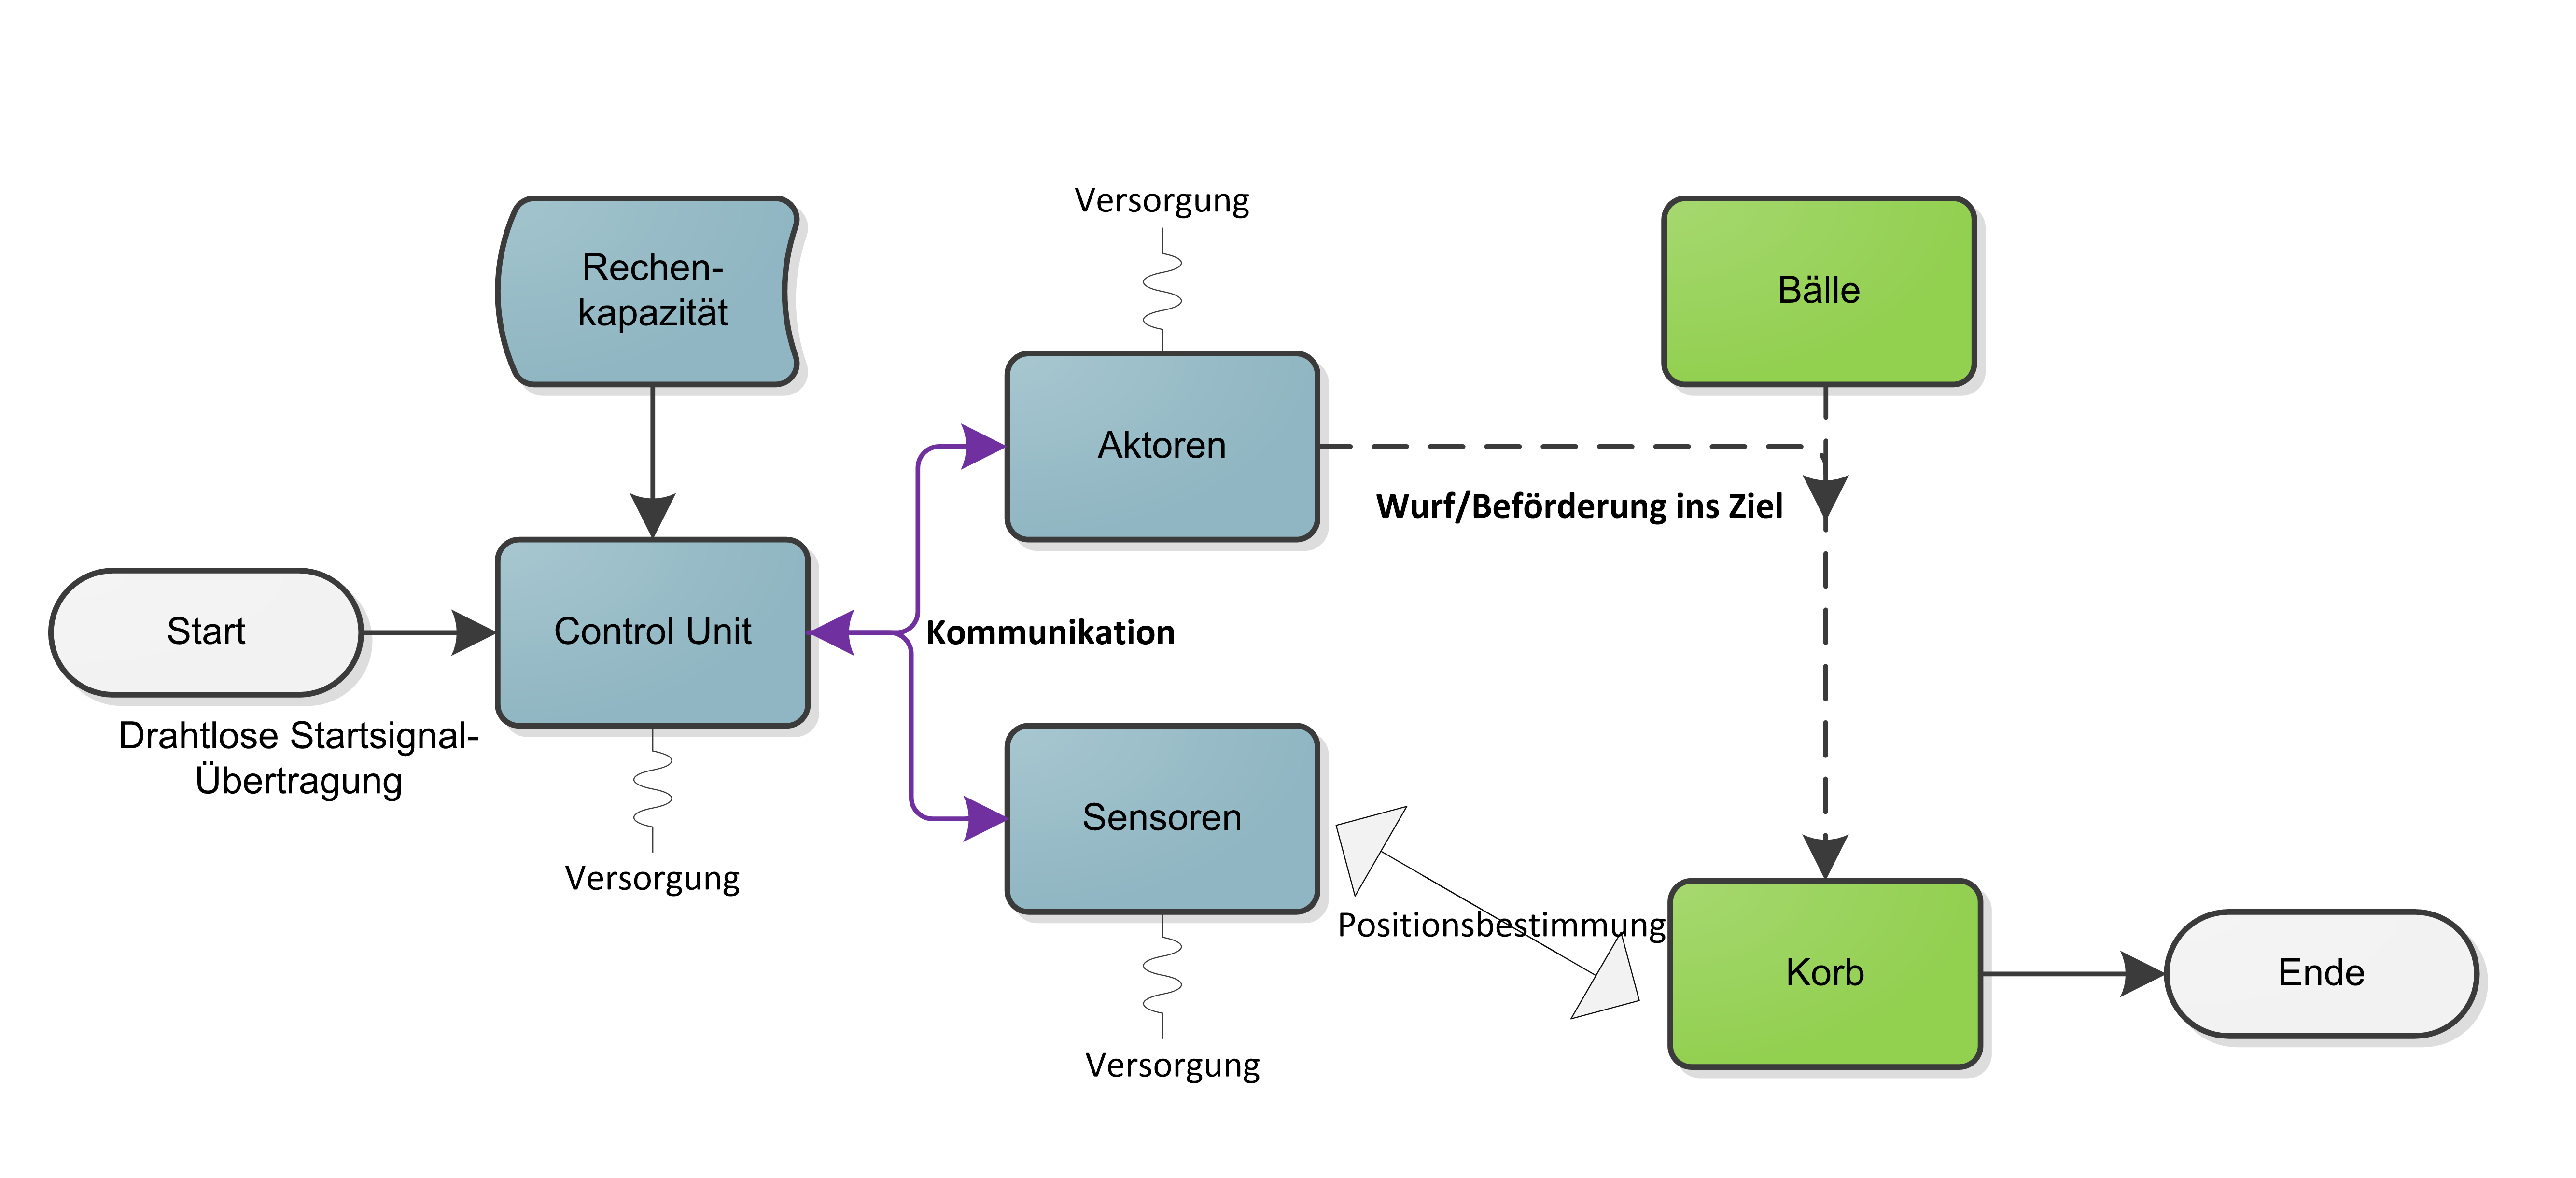
\includegraphics[width=1\textwidth]{Enddokumentation/Varianten/Bilder/Funktionsskizze.png}
	\caption{Funktionsskizze}
	\label{fig:Funktionsskizze}
\end{figure}
\\
Nach der Ermittlung dieser Teilprobleme mussten für die einzelnen Bereiche nach Lösungsansätzen
recherchiert werden. Die Resultate dieser Recherche, sowie die danach folgende Bewertung der
gefundenen Lösungen ist aus Platzgründen im Anhangsdokument hinterlegt. Um die Ergebnisse der Bewertung
sinnvoll als Entscheidungshilfe einsetzen zu können, wurden sie kompakt zu einem Grobkonzept
zusammengefasst.\\
\\
Jedes Teilproblem ist bezüglich den Vor- und Nachteilen nach den definierten Zielsetzungen
bewertet worden. Dadurch lassen sich grafisch geeignete Kombinationsmöglichkeiten herleiten und
untereinander vergleichen. Um möglichst vielen differenzierten Ansätzen Rechnung zu tragen,
wurden vier Varianten während einer Diskussionsrunde festgelegt.
\newpage
\begin{figure}[t]
	\centering
	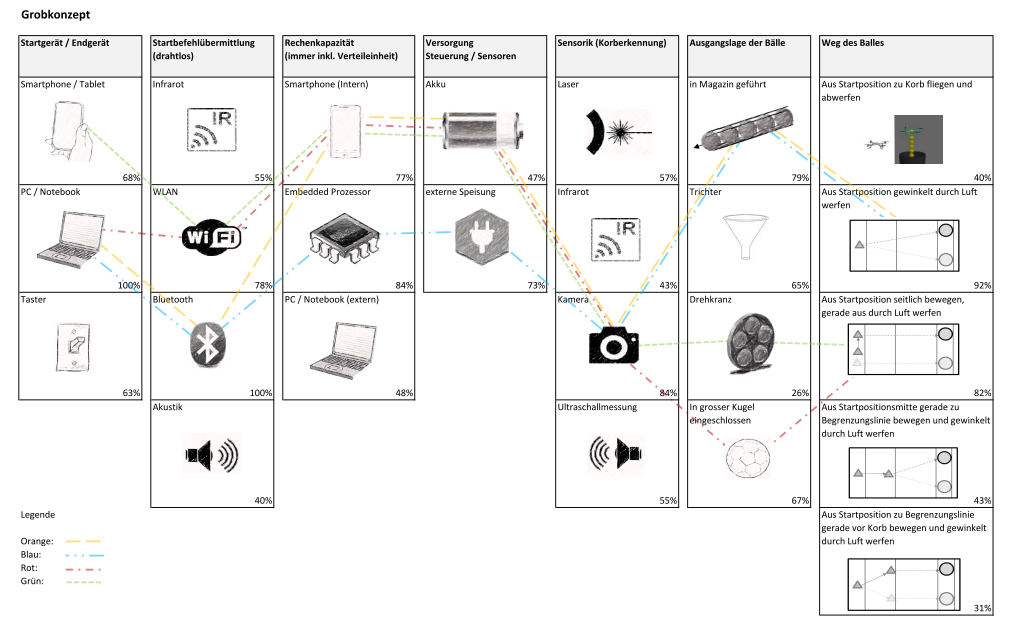
\includegraphics[width=1.08\textwidth]{Enddokumentation/Varianten/Bilder/Grobkonzept.png}
	\caption{Lösungsansätze für die einzelnen Teilprobleme mit den vier gewählten Varianten}
	\label{fig:Grobkonzept}
\end{figure}
\noindent Die blaue Variante ist die Kombination aller Lösungsansätze mit der höchsten
Prozentzahl. Die rote Variante basiert auf der Idee, die Bälle in eine Kugel einzuschliessen,
das Gerät parallel zur Spielfeldwand zu verschieben und den Korb mit einer Smartphone-Kamera zu
erkennen. Der Ballwerfer soll durch einen Akkumulator mit Energie versorgt werden. Als
Ausgangslage führt die grüne Variante die Bälle in einem Drehkranz und befördert diese einzeln
in den Korb, die restlichen Kriterien werden kongruent zur zweiten Variante ausgeführt. Im
orangen Konzept befördert der Ballwerfer die Bälle aus der Startposition in bogenförmiger Kurve in den Korb. Die Ausgabe der Bälle erfolgt vereinzelt. Die übrigen Teilprobleme verwenden
wiederum, äquivalent zur zweiten Variante eine Smartphone-Kamera zur Korberkennung und einen
Akkumulator als Energieversorgung.\\
\\
Die Entscheidung fiel auf die orange Variante. Diese bietet als gesamtes Konzept die
erfolgversprechendste und effizienteste Lösung, bezüglich der Zielsetzung des Teams. \\

\begin{tabular}{p{1cm}p{10cm}}
	\multirow{3}{4cm}	{
\includegraphics[width=1cm]{Enddokumentation/Varianten/Bilder/info_icon.png}}
	 & Die detaillierte Beschreibung der Lösungsfindung (von der Funktionsskizze bis zum
	 Feinkonzept) war Aufgabe des zweiten Testates und ist als Dokument im Anhangsdokument beigelegt. \\
\end{tabular}\\
\\
\\
Nach der Entscheidung für eine Variante folgt die weitere Ausarbeitung des Konzeptes
in einzelne Feinkonzepte. Die ursprünglich sieben Teilprobleme wurden in 19 Subteilprobleme
aufgesplittet. Zu jedem Subteilproblem existieren wiederum Lösungsvarianten. Im Unterschied 
zum Grobkonzept erfolgt die Bewertung nicht mit Prozenten, sondern werden die Lösungsvarianten
miteinander verglichen und nach aktuellem Wissenstand eine oder eventuell auch mehrere
Lösungsvarianten ausgewählt. 



    %
    % Lösungskonzept
    %
    \newpage
    \section{Lösungskonzept}
Als Hauptteil der Arbeit umfasst das Lösungskonzept Beschreibungen von erfüllten Funktionen und verbauten Komponenten, sowie 
grundlegende Berechnungen für den autonomen Ballwerfer. Die Strukturierung des Kapitels \ref{shap:Geraeteuebersicht} erfolgt dabei in der Reihenfolge, in welcher die Komponenten zur Lösung der Aufgabe benötigt werden.
    \subsection{Funktionsbeschreibung}
Der Ballwerfer befindet sich in der Ausgangsposition in der Startfeldmitte. Nach einer drahtlosen Übermittlung des Startsignals beginnt das Smartphone auf dem Ballwerfer mit der Korberkennung. Zeitgleich werden die Schwungräder auf ihre Nenndrehzahl beschleunigt. Durch die Auswertung des fotografierten Bildes wird die Position des Korbes ermittelt und aus dieser einen Winkel für die Justierung der Abwurfeinheit des Ballwerfers berechnet. Nach der Übermittlung des Winkels an den Controller richtet der Stellantrieb die Abwurfeinheit in die gewünschte Wurfposition aus. Ein Förderband befördert anschliessend die Bälle zu den Schwungrädern, wo diese auf ihre Abwurfgeschwindigkeit beschleunigt werden. Die Bälle verlassen nacheinander das Gerät und fliegen in einer Wurfparabel direkt in den Korb. Sobald sich alle Bälle im Korb befinden (zeitabhängig), wird das akustische Endsignal auf dem Smartphone ausgegeben.
\begin{figure}[h!]
	\centering
	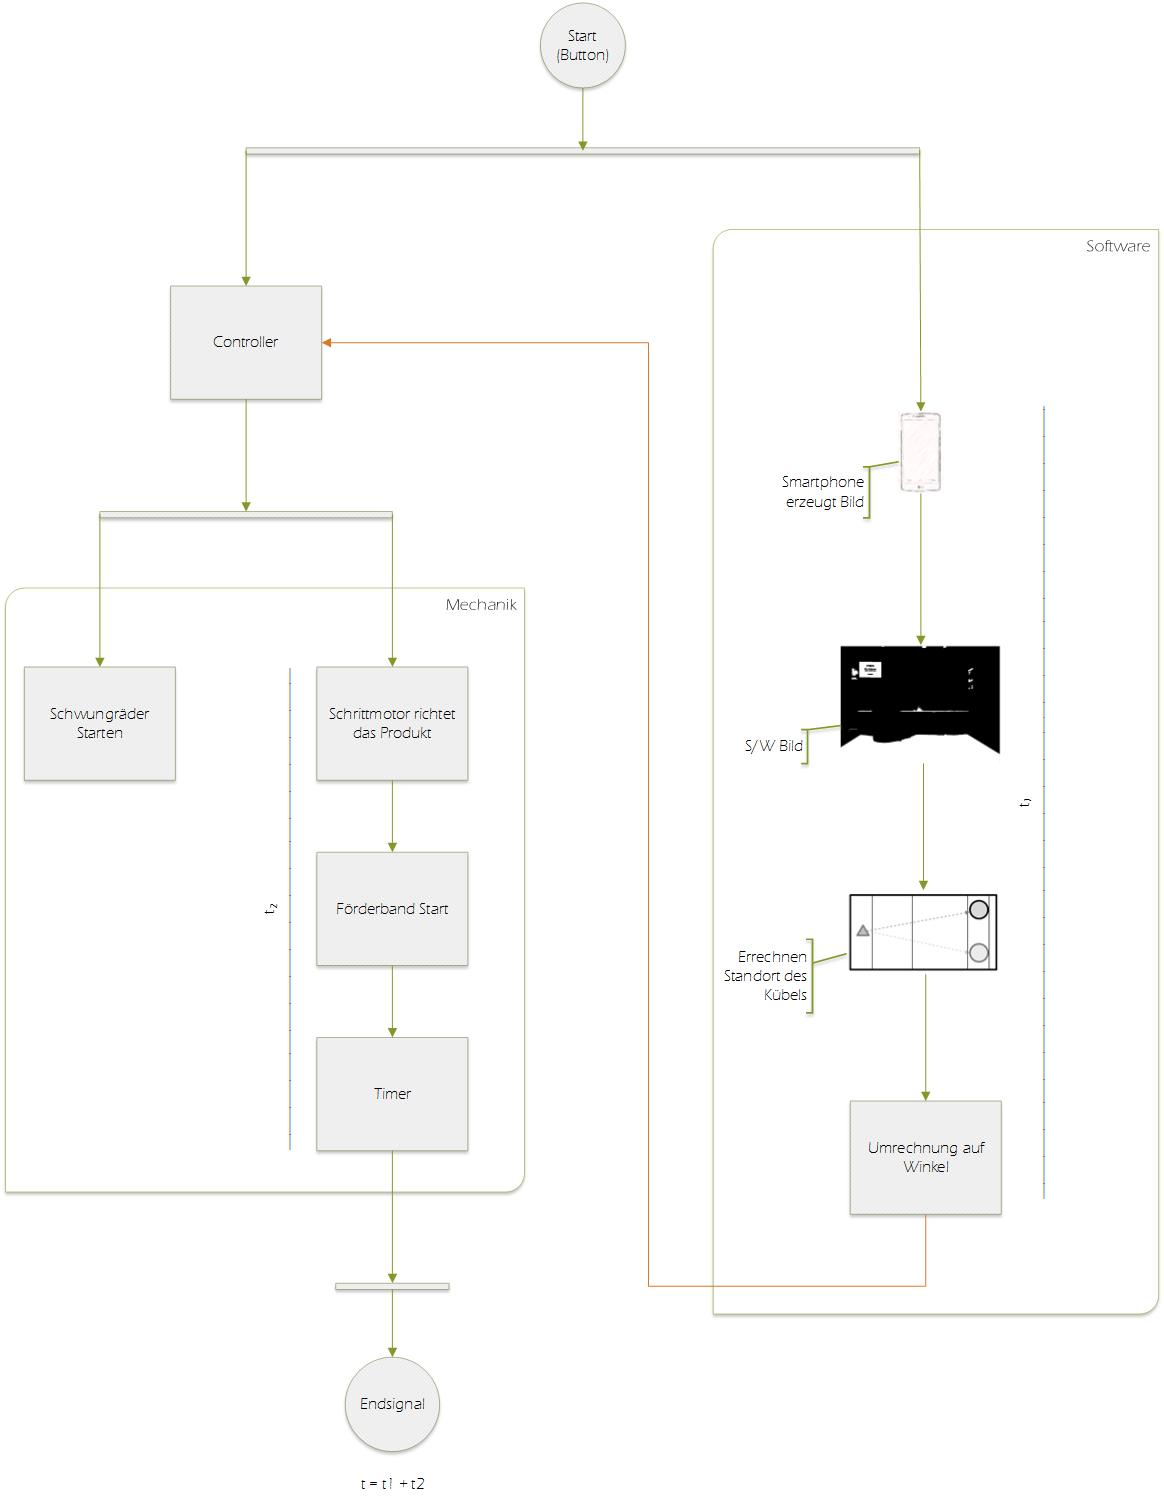
\includegraphics[width=0.9\textwidth]{Enddokumentation/Loesungskonzept/Bilder/FlowOnChart_v2.jpg}
	\caption{Funktionsskizze}
	\label{fig:FlowChart}
\end{figure}
Die Grafik stellt den schematischen Ablauf der oben erwähnten Funktionen dar. Einige Teilschritte des Ablaufes, wie zum Beispiel das Beschleunigen der Schwungräder werden je nach zeitlicher Dauer oder möglich auftretenden Störungen (in Form von Vibrationen) verschoben.
    \newpage
    \subsection{Geräteübersicht}
Der Ballwerfer ist so konzipiert, dass er aus einem fixstehenden Basismodul besteht, welches in der Mitte des Startbereiches positioniert wird. Die Abwurfeinheit, welche den Ballwurfmechanismus und die Ballzuführung beinhaltet, ist auf dem Basismodul drehend gelagert. Ein Schrittmotor richtet die Abwurfeinheit auf das Ziel aus. Der ganze Aufbau des Ballwurfmechanismus ist möglichst einfach gehalten. Er besteht Hauptsächlich aus zwei Acrylglasplatten, in welcher alle mechanischen Vorrichtungen gelagert sind. Dadurch kann der ganze Aufbau schnell und einfach angepasst oder geändert werden. Die Ausrichtung des Abwurfmechanismus erfolgt durch einen Schrittmotor, welcher in der drehenden Abwurfeinheit angebracht ist. Dadurch kann die Bauhöhe des Ballwerfers tief gehalten werden, was einen grossen Stabilitätsvorteil bietet. Die Drehachse am vorderen Ende der Abwurfeinheit ist an der Spitze des Ballwerfers mit einem Bolzens angebracht. Somit bleibt die Abwurfposition der Tennisbälle konstant am gleichen Ort.\\
Die Tennisbälle werden durch zwei Schwungräder beschleunigt. Die Schwungräder drehen gegenläufig, der Tennisball wird dazwischen ausgestossen. Die Zuführung der Tennisbälle erfolgt mit einem eigens geregelten Förderband. Das Förderband muss die Bälle mit konstanter Geschwindigkeit zu den Schwungrädern transportieren, damit alle Tennisbälle die gleiche Startenergie aufweisen. Dadurch ist eine gleichmässige Wurfweite und eine hohe Reproduzierbarkeit gewährleistet. \\
\begin{figure}[h!]
		\centering
		\includegraphics[width=0.9\textwidth]{Enddokumentation/Loesungskonzept/Bilder/Geraeteuebersicht.jpg}
		\caption{Geräteübersicht}
		\label{fig:Geraeteuebersicht}
\end{figure}}\\
\begin{figure}[h!]
	\centering
	\caption{Bezeichnung der Teilkomponenten}	
	\label{tab:BezTeilkomponenten}
	\begin{tabular}{|c|c|c|}
		\hline Pos & Bezeichnung & Funktion \\ 
		\hline 1 & Startgerät (Smartphone) & Senden Startbefehls, Empfangen Endbefehl, Akustische,visuelle Signalausgabe
		\\ 
		\hline 2 & Master  (Smartphone) & Empfangen des Startbefehls, Senden Endbefehl
		Fotografieren und Auswerten, Steuern des Controllers
		\\ 
		\hline 3 & Controller & Steuerung und Regelung der Antriebe \\ 
		\hline 4 & Gestell & Stabilisieren des Systems
		Seitliche Führung der Bälle
		\\ 
		\hline 5 & Stelleinheit & Ausrichten des Gerätes zum Korb \\ 
		\hline 6 & Förderband & Ballförderung zu Schwungräder \\ 
		\hline 7 & Schwungräder inkl. Antrieb & Beschleunigen der Bälle \\ 
		\hline 
	\end{tabular} 
\end{figure}\\
In den folgenden Abschnitten wird nach dem zeitlichen Ablauf des Balles, die einzelnen Komponenten des Ballwerfers näher beschrieben. 
    \subsubsection{Startgerät}
    \subsubsection{Smartphone als Master}
	Ein Smartphone vereint mehrere für die Realisation des Produkts benötigte Komponenten (Kamera, drahtlose Schnittstelle, Recheneinheit, Endsignalausgabe) 
	in einem Gerät. Des Weiteren sind heutige Smartphones verhältnismässig leistungsfähig, die Berechnungen für die Objekterkennung 
	können direkt auf dem Gerät erfolgen und durch den USB-Port wird eine sichere Verbindung zum Controller gewährleistet. Die Alternative, einzelne Module (Kamera, drahtlose Schnittstelle, Recheneinheit) zu verbauen, 
	gewährleistet eine erhöhte Flexibilität, allerdings verbunden mit steigendem Aufwand und höherem Preis. 
	Zudem hätte die Verwendung von Einzelmodulen unter Umständen eine Gewichtszunahme zur Folge, da keine vergleichbare Kompaktheit wie bei einem Smartphone besteht. 
	Der Einsatz eines Smartphones bietet im Vergleich zu einzelnen Modulen somit entscheidende Vorteile.\\
	\\
	Es ist wichtig, dass die Kamera das Spielfeld komplett erfassen kann, weswegen das Smartphone vorne am Gerät angebracht wird. 
	Eine Befestigung an der Front des Gerätes bietet sich an, da dort eine hohe Stabilität vorhanden ist, 
	was für eine optimale Bildaufnahme wichtig ist.\\
	\\
	Falls die Korberkennung nicht auf dem Smartphone implementiert werden kann, 
	wird die Berechnung auf einem externen PC durchgeführt. In diesem Fall wird eine Webcam am PC 
	angeschlossen. Die Montage an der Abwurfeinheit bleibt am selben Ort wie das Smartphone bestehen. Die Kommunikation 
	zwischen PC und dem Controller wäre wie beim Smartphone über USB realisiert.
	%
	\paragraph{Korberkennung}$~~$\vspace{2mm}\\
		Für die Bestimmung der Position des Korbes wurde ein Algorithmus entwickelt und in Java implementiert. 
		Dieser ist in Abbildung \ref{fig:KorberkennungFlowchart} grafisch dargestellt. Der Algorithmus basiert 
		auf der Tatsache, dass der Korb deutlich dunkler als der Hintergrund ist. Dies konnte anhand eines 
		Testversuches unter variablen Lichtbedingungen bestätigt werden. Der Versuch ist in Kapitel \ref{chap:ListTest} aufgeführt.
		Um mit dem von der Kamera zuvor aufgenommenen Bild arbeiten zu können, müssen die Ränder abgeschnitten werden 
		(vor allem links und rechts geht der Bildbereich über das Spielfeld hinaus, was das Resultat verfälschen könnte). 
		Als zweiter Schritt wird über sämtliche Pixel des Bildes iteriert. Dabei wird für jedes Pixel die Helligkeit bestimmt 
		anhand einer vordefinierten Schwelle entschieden, ob es zum Hintergrund (heller) oder zum Korb (dunkel) gehört. 
		Anschliessend wird der Schwerpunkt der dunklen Pixel bestimmt und anhand des gefundenen Schwerpunktes entweder
		von links oder von rechts her in einem bestimmten horizontalen Bereich (der Korb befindet sich immer auf der selben Höhe)
		über die Pixel iteriert um dabei eine feste Kontur zu finden. Diese feste Kontur wird dabei definiert durch eine
		bestimmte Anzahl weisse Pixel, auf welche wiederum eine Menge schwarzer Pixel folgen muss. 
		Da dieser Prozess immer in derselben horizontalen Ebene stattfindet kann durch eine abschliessende Berechnung 
		der Mittelpunkt des Korbes und der damit verbundene Winkel des Ballwerfers zum Korb trigonometrisch bestimmt werden.
		\begin{figure}[h!]
			\centering
			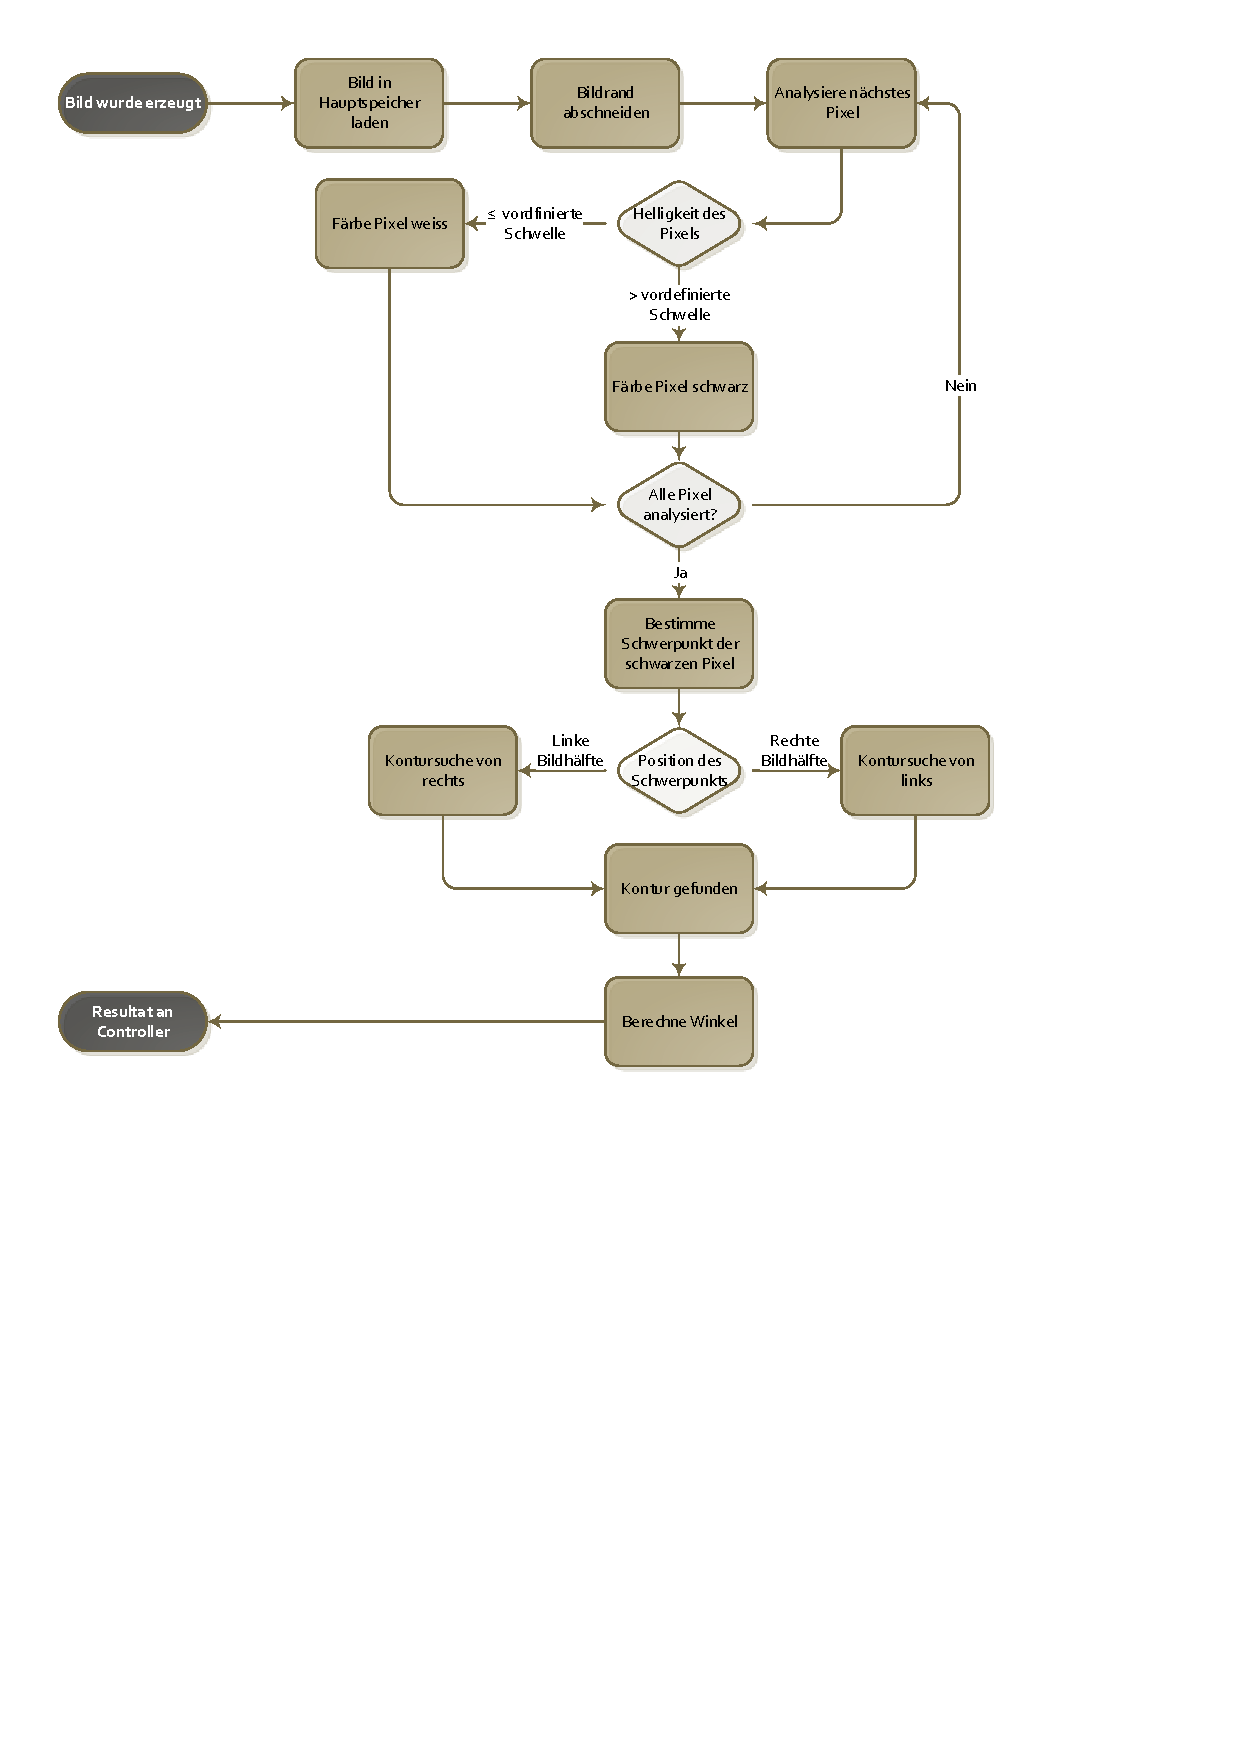
\includegraphics[width=1\textwidth,clip,trim=9mm 115mm 41mm 9mm]
			{Enddokumentation/Loesungskonzept/Bilder/Flowchart_Korberkennung.pdf}
			\caption{Ablaufdiagramm zum Korberkennungs-Algorithmus}
			\label{fig:KorberkennungFlowchart}
		\end{figure}
    \subsubsection{Controller}
\label{sec:Controller}
	Die Controller-Hardware steuert die Motoren der Ballzuführung, der Stepper für die Ausrichtung 
	der Abwurfeinheit und die Motoren zur Beschleunigung der Bälle. Sobald der Controller das Startsignal vom Smartphone erhält, 
	wird dieser den Motor der Schwungräder aktivieren und auf Nenndrehzahl drehen lassen. Weiter erhält der Controller vom Master die Angabe, 
	in welchem Winkel sich der Korb zum Gerät befindet. Anhand dieser werden die benötigten Schritte berechnet und die resultierenden Befehle 
	an die Motorsteuerung werden abgesetzt. Sobald die Abwurfeinheit die richtige Position eingenommen hat, wird die Ballzuführung aktiviert. 
	Mit einem Sensor werden die Bälle gezählt und sobald der letzte Ball abgefeuert wurde, wird dies dem Master wiederum signalisiert zur Ausgabe des Endsignals.\\
	\begin{wrapfigure}{r}{0.45\textwidth}
		\centering
		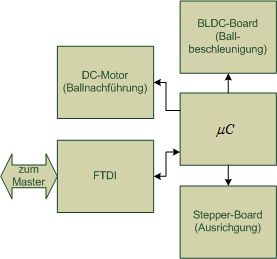
\includegraphics[width=0.44\textwidth]{Enddokumentation/Loesungskonzept/Bilder/Blockschaltbild_Controller.png}
		\caption{Blockschaltbild der Controller-Hardware}
		\label{fig:Blockschaltbild_Controller}
	\end{wrapfigure}
	Die Abbildung \ref{fig:Blockschaltbild_Controller} zeigt auf, wie die Controller-Hardware aufgebaut wird. 
	Die Brushless-Motor- und Stepper-Ansteuerung wird auf separaten Boards realisiert, wobei die Stepper-Hardware durch die PREN-ET-Gruppe
	entwickelt und in dieser Gruppe eingesetzt wird. Als Schnittstelle zwischen den Boards und dem Controller wird SPI\footnote{\textbf{S}erial \textbf{P}eripheral \textbf{I}nterface, Dabei handelt es sich um ein synchronen seriellen Datenbus} eingesetzt, 
	da ein Hauptchip der Stepper-Ansteuerung nur über SPI angesprochen werden kann. Die Kommunikation mit dem Smartphone wir über UART\footnote{\textbf{U}niversal \textbf{A}synchronous \textbf{R}eceiver \textbf{T}ransmitter, Dabei handelt es sich um ein asynchrone serielle Schnittstelle} stattfinden, 
	das über den FTDI-Chip auf USB emuliert wird. Die Ansteuerung des DC-Motors wird mittels PWM\footnote{\textbf{P}ulse \textbf{W}idth \textbf{M}odulation, Pulsweitenmodulation} realisiert.
    \subsubsection{Grundaufbau Mechanik}
    \subsubsection{Stelleinheit}
Um die Abwurfeinheit zum Ziel auszurichten, wird ein verstellbarer Mechanismus benötigt, der eine hohe Genauigkeit aufweist. Der Drehpunkt muss sich möglichst unter den Schwungrädern befinden, damit die 
Position des Abwurfes im Zentrum des Spielfeldes bleibt. Die Drehung wird mit einen Schrittmotor
realisiert. Ein Schrittmotor bietet sich hier an, da somit eine sehr exakte Ansteuerung gewährleistet
wird. Dadurch kann der Verstellwinkel, welcher von der Position des Zieles abhängt, genau eingestellt
werden. Der Schrittmotor wird in der Abwurfeinheit angebracht und treibt ein Ritzel an, welches in
einen Zahnkranz eingreift. Dadurch kann die Abwurfeinheit gedreht werden. Damit die Bauhöhe nicht
zusätzlich vergrössert wird, ist der Zahnkranz in die Bodenplatte integriert. Die Bodenplatte mit dem
Zahnkranz reicht nicht über die ganze Abwurfeinheit, damit die Masse möglichst klein gehalten werden
kann. Der Schrittmotor ist nach dem folgenden Drehmoment von ca. $2 Nmm$ ausgelegt. Dies ist sehr klein,
da nur der Reibungskoeffizient und die Normalkraft, welche vom Gewicht der Abwurfeinheit abhängt, das
Moment erzeugen. Der Reibungskoeffizient wird durch die Lagerung klein gehalten. Die Lagerung erfolgt
im Drehzentrum durch eine Hülse und im Endbereich der Abwurfeinheit durch zwei Kugelrollen, welche mit
einem seitlichen Abstand angebracht sind. Dadurch ist auch die Gefahr, dass die Abwurfeinheit kippen
könnte gebannt. Die Ansteuerung der Schrittmotoren erfolgt über den selbst konstruierten Controller.
\begin{figure}
	\centering
	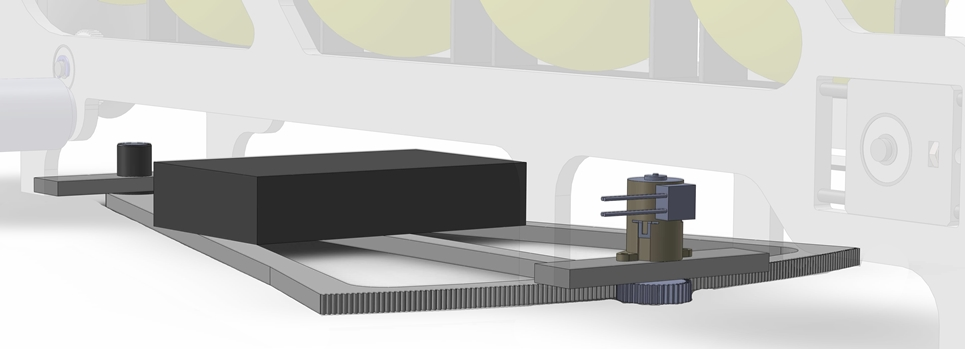
\includegraphics[width=0.9\textwidth,clip,trim=0mm 0mm 0mm 0mm]
	{Enddokumentation/Loesungskonzept/Bilder/Stelleinheit.jpg}
	\caption{Grafik des Antriebes}
	\label{fig:GrafikDesAntriebes}	
\end{figure}
    \subsubsection{Förderband}
Da die Schwungräder durch den Abwurf um ca. 40\% (Berechnung in Formel \ref{equ:AbbremsungBall} im
Anhang) abgebremst werden, müssen sie nach jedem Wurf erneut auf die gewünschte Drehzahl
beschleunigt werden. Deshalb hat die Zuführung der Bälle in Abständen zu erfolgen. Weiter müssen die
einzelnen Tennisbälle immer mit der gleichen Geschwindigkeit bei den Schwungrädern eintreffen, damit
eine konstante Wurfweite entsteht. Die beste Art, beides zusammen zu realisieren ist ein Förderband.
Das Förderband wird zwischen den zwei Acrylglasplatten aufgespannt. Der Antrieb des Förderbandes
erfolgt mit einem DC-Motor. Dieser wird mit einem Verhältnis von $i=5:1$ untersetzt, um das benötigte
Drehmoment an die Antriebstrommel zu übertragen. Die Berechnungen dazu sind im Anhang in Formel
\ref{equ:M_Antrieb} ff. ersichtlich. Auf dem Förderband, welches aus einem
Flachbandriemen besteht, sind konvexe Führungsschaufeln angebracht. Diese sind so ausgerundet, damit
der Ball möglichst lange geführt werden kann und die Führungsschaufeln nicht in Berührung der
Schwungräder kommen. Die Schaufeln werden voraussichtlich mit dem Förderband verschweisst.
\begin{figure} [h!]
	\centering
	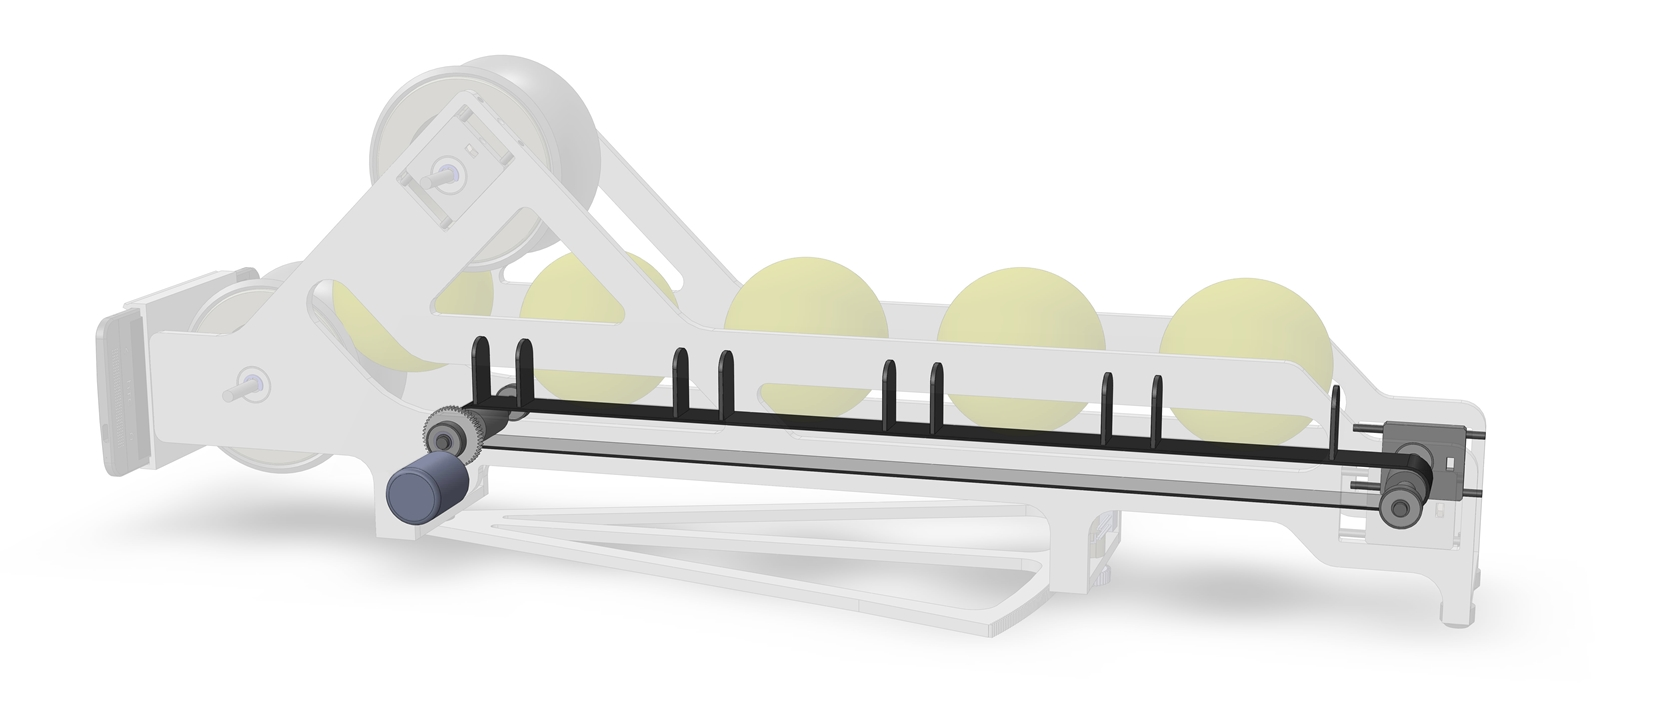
\includegraphics[width=0.9\textwidth,clip,trim=0mm 0mm 0mm 0mm]
	{Enddokumentation/Loesungskonzept/Bilder/Foerderband.jpg}
	\caption{Grafik Förderband}
	\label{fig:GrafikFörderband}	
\end{figure}
Aus Testversuchen der Ballzuführung wurde erkannt, dass für einen idealen Abwurf beide Räder
zeitgleich den Ball einklemmen müssen. Somit müssen die Bälle zunächst unterhalb des oberen
Schwungrades gefördert und anschliessend in einem 45$^\circ$ Winkel nach oben zugeführt werden. Dazu dient
ein Führungselement. Die Gestaltung dafür wird sich durch Tests zeigen. Als Ideen stehen zwei
Stangen oder ein Blech, welches die Bälle zu den Schwungrädern führt zur Auswahl. Die Abbildung
\ref{fig:GrafikFörderband} zeigt ein mögliche Ausführung der Schaufeln am Band.
    \subsubsection{Schwungräder}
    \subsection{Versorgungskonzept}
	Das Smartphone, die Controller-Hardware und die Motoren benötigen jeweils bestimmte Spannungen, die erzeugt werden müssen. Diese werden aus einer Hauptspannung generiert. Die Spannung kann von Akkumulatoren oder einem externen Netzgerät bezogen werden. Da das Gewicht der Spannungsversorgung beim Wiegen nicht dazu gezählt wird, könnten Akkumulatoren allenfalls als Ballastgewicht eingesetzt werden. Sollte sich zeigen, dass zusätzliches Gewicht nötig ist um den Ballwerfer zu stabilisieren, werden Akkumulatoren eingesetzt. Ansonsten wird die benötigte Spannung von einem Netzgerät bezogen. Der benötigte Strom ist massgeblich vom Brushless-Motor abhängig. der  Strombedarf der Controller-Hardware kann im Vergleich des Motors vernachlässigt werden.
    \subsection{Hardware}
    Die Elektrotechnik-Studierenden aus mehreren Gruppen haben sich zusammengeschlossen um gemeinsame Probleme anzugehen. Dabei handelt es sich um die Ansteuerung, die benötigte Hard- und Software um Motoren anzusteuern und gegebenenfalls zu regeln. In diesem Zusammenschluss wurde drei Gruppen gebildet, um Lösungen für DC-, Stepper- und Brushless-Motoren auszuarbeiten. Die Idee besteht darin, dass nicht jede Gruppe für dasselbe Problem wo möglich denselben Lösungsansatz verfolgt, sondern die Ressourcen kombiniert, Synergien nutzt um eine bessere Lösung zu erarbeiten. Auf diese Weise kann das Team übergreifende Arbeiten im Rahmen der \enquote{PREN} erlernt und geübt werden. Somit wird Idee der Interdisziplinarität im erweiterten Sinn Rechnung getragen. Die Gruppen und deren Mitglieder sind in der folgenden Aufzählung ersichtlich:
    \begin{itemize}
        \item[$\star$] DC-Motoren-Gruppe\\
            Besteht aus Elektronik Student des Teams 39.
        \item[$\star$] Stepper-Motoren-Gruppe\\
            Besteht aus den Elektronik Student des Teams 38 und 27.
        \item[$\star$] Brushless-Motoren-Gruppe\\
            Besteht aus den Elektronik Studenten des Teams 27 und 32.
    \end{itemize}
    \subsection{Software-Architektur}
	\subsubsection{Systemübersicht}
	Zur Übersicht über den erarbeiteten Lösungsansatz bietet sich die Darstellung durch ein Kontextdiagramm an. Darin zu erkennen sind die fünf Hauptkomponenten  DesktopViewer, CoreApp, Detector, MediaCommunication und ControllerCommunication. Weiter enthält das System mindestens drei Schnittstellen, einerseits die Bluetooth Schnittstelle zwischen Startgerät und Ballwerfer, des weiteren muss die Kommunikation mit Kamera und Controller gewährleistet sein.\\ 
	Die Schnittstelle zur Kamera sollte, wenn wie geplant ein Smartphone verwendet wird, bereits durch das entsprechende Betriebssystem gegeben sein, weshalb in diesem Dokument nicht weiter auf diese Schnittstelle eingegangen wird. 
\begin{figure}[h!]
		\centering
		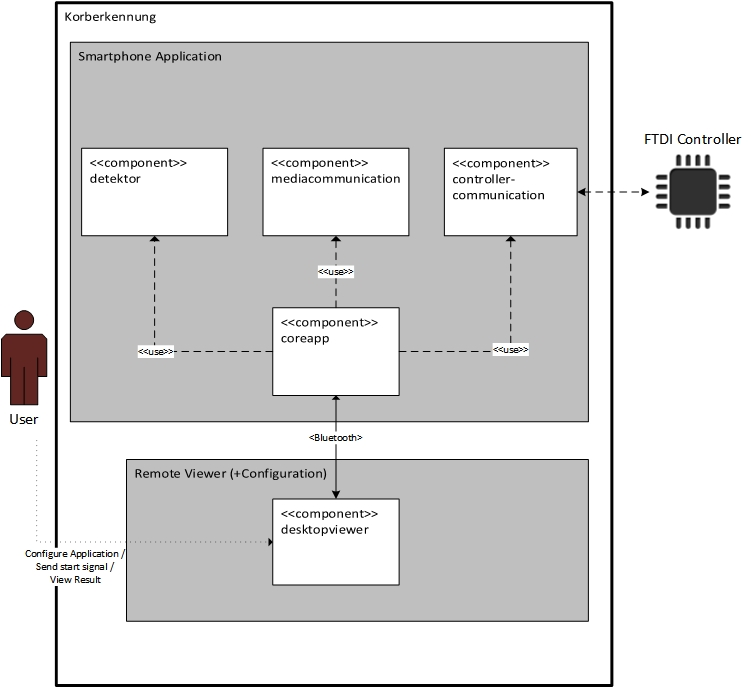
\includegraphics[width=0.9\textwidth]{Enddokumentation/Loesungskonzept/Bilder/Kontextdiagramm_v2.jpg}
		\caption{Kontextdiagramm}		
\end{figure}


	\subsubsection{Komponenten-Spezifikation}
		\paragraph{DesktopViewer}$~~$\vspace{2mm}\\
		Über die Viewer-Komponente wird die Konfiguration der Applikation, sowie die Auslösung des Startsignals realisiert. Optional soll es zu Testzwecken möglich sein, die Resultate der Korberkennung ebenfalls über den DesktopViewer zu betrachten.
		
		\paragraph{CoreApp}$~~$\vspace{2mm}\\
		Als Kernbestandteil der Smartphone App umfasst die CoreApp-Komponente auf der einen Seite die Kommunikation mit der Viewer-Komponente, auf der anderen Seite wird hier der Ablauf der Kernfunktionen zur Objekterkennung koordiniert.		
		
		\paragraph{MediaCommunication}$~~$\vspace{2mm}\\
		In dieser Komponente ist die Kommunikation mit der Kamera des Smartphones und die Wiedergabe des Endsignals zuständig. MediaCommunication nimmt ein Foto auf und stellt dieses für die Winkelberechnung bereit, auf ein eintreffendes Endsignal wird ein Akustisches Signal ausgegeben was signalisiert das alle Bälle die Maschine verlassen haben.
		
		\paragraph{Detector}$~~$\vspace{2mm}\\
		Dem Detektor muss ein Bild übergeben werden, welches von diesem darauf ausgewertet wird. Dabei sucht der Detektor nach einem dunkeln Objekt im Bild und ist in der Lage, anhand der ermittelten Position den Winkel des Ballwerfers zum Korb bestimmen kann.
		

		\paragraph{ControllerCommunication}$~~$\vspace{2mm}\\
		Wie der Name bereits sagt wird an dieser Stelle die Kommunikation mit dem FTDI-Controller realisiert. Der vom Detektor berechnete Winkel wird hier an den FTDI-Controller übertragen. Anschliessend wartet die Komponente bis der Controller ein Endsignal zurückgibt welches das Ende des Ballwurfs signalisiert.
		
	\subsubsection{Schnittstellen-Spezifikation}
		% Übersicht Schnittstellen fehlt Schnittstellen
		\begin{figure}[h!]
			\centering
			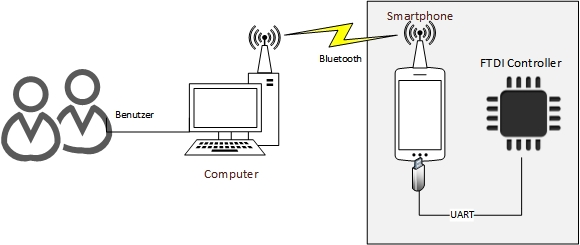
\includegraphics[width=0.9\textwidth]{Enddokumentation/Loesungskonzept/Bilder/Schnittstellen.jpg}
			\caption{Schnittstellen}		
		\end{figure}
		Als weiteres Hauptelement des entworfenen Systems werden im nachfolgenden Abschnitt die in der Grafik erkennbaren Schnittstellen (Bluetooth und Controller) deklariert.
		
		\paragraph{Bluetooth}$~~$\vspace{2mm}\\
		Die Kommunikation vom Startgerät (Notebook) zum Smartphone (Android Device auf dem Ballwerfer) für die Übermittlung des Startsignals findet mit Bluetooth statt. Die Bluetooth-Komponente auf dem Notebook startet nach Aktivierung ein ‚inquiry‘ (Erkundigung) nach verfügbaren Bluetooth-Geräten. Anschliessend wird eine Service-Anfrage (RFCOMM, eine COM-Schnittstelle) an ein gewünschtes Bluetooth-Gerät gestartet, bei positiver Rückmeldung werden die zwei Geräte gepaart. Eine uni- oder bidirektionale Kommunikation zwischen den Geräten kann nun jederzeit aufgebaut werden. Das eigentliche Startsignal wird ein primitiver Datentyp sein.
		
		\paragraph{Controller}$~~$\vspace{2mm}\\
		Die Verbindung vom Android Smartphone zum FTDI Controller wird mit USB realisiert. 
		Das Smartphone kommuniziert über den bereitgestellten Treiber von FTDI mit dem Controller, die verwendete Schnittstelle ist UART. Die Kommunikation soll bidirektional sein, kann sowohl empfangen als auch senden. Der Vorteil einer solchen Verbindung ist, dass sie als COM-Schnittstelle angesteuert werden kann was relativ einfach zu implementieren ist. Die Verbindung ist ausfallsicher und einfach aufrechtzuerhalten.		
		
	\subsubsection{Funktionale Sicht}
	
	\begin{figure}[h!]
		\centering
		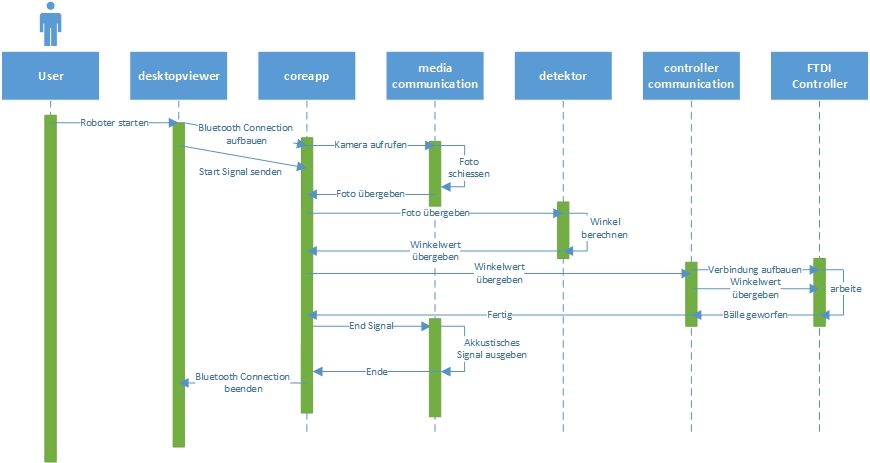
\includegraphics[width=0.9\textwidth]{Enddokumentation/Loesungskonzept/Bilder/Sequenzdiagramm.jpg}
		\caption{Sequenzidagramm}		
	\end{figure}
Ein User gibt den Startbefehl für den Roboter durch die Komponente desktopviewer, die auf einem Computer(Laptop) ausgeführt wird. Desktopviewer baut eine Bluetooth-Connection mit der Komponente Coreapp auf, welche auf dem Smartphone ausgeführt wird, und sendet anschliessend das Startsignal welches durch den User ausgelöst wird. \\
Ab diesem Zeitpunkt läuft die Applikation völlig autonom. Die coreapp ruft als erstes die mediacommunication Komponente auf und schiesst ein Foto. Coreapp ruft die Komponente 	detektor auf und übergibt dieser das Foto, welche daraufhin den Winkel ausrechnet.\\
Der berechnete Winkel wird an die Komponente controllercommunication übergeben. Die Komponente baut die Verbindung zum FTDI-Controller auf und übergibt diesem den Winkelwert, danach wartet die Komponente bis der FTDI-Controller das Ende des Ballwurfes zurückgibt. Die Komponente controllercommuncation übergibt an die Coreapp die Meldung das der Roboter fertig ist. \\
Coreapp ruft die medacommunication Komponente auf welche das Programmende signalisiert.
		
		

%    %
    % Tests
    %
    \newpage
    \section{Tests}
    \subsection{Zylinder-Test}
\begin{tabular}{p{2cm}p{2cm}}
	Typ: & Pneumatikzylinder \\
	Datum: & 8.10.2014     \\
	Ort: & Bachmann Engineering AG (Zofingen)   \\
	Tester: & Gruppe 32     \\
	
\end{tabular}



Ziel des Testes:   \\
Der gebaute Prototyp soll auf die 
Wurfwiederholgenauigkeit getestet werden. 
Fazit/ Verbesserungsvorschlag: \\
Ein Pneumatikzylinder arbeitet sehr zielgenau und schnell. 
Zu verbessern: 
Es wurde ein überdimensionierter Zylinder für die Testzwecke verwendet.  \\

%\rightarrow benötigte Abschussgeschwindigkeit mittels schiefer Wurf bestimmen. 
Anschliessend mittels Stoss die benötigte Beschleunigung des Zylinders 
bestimmen und im Anschluss den Zylinder gemäss ausgerechneten Daten 
(Druckversorgung / Kolbendurchmesser / Drosselung) auslegen. \\

Mit einem kleineren kann an Gewicht und Kosten gespart werden. Als 
Ansteuerung reicht ein federrückgestelltes Magnetventil.  \\
Ziel erreicht:   JA
    \subsection{Schwungrad-Test}
    \subsection{Drehzahl-Test}
    \subsection{Brushless-Motor-Test}
    \subsubsection{Brushless Motoransteuerung}
\textbf{Theorie der Ansteuerung}:\\
\begin{wrapfigure}{r}{0.50\textwidth}
	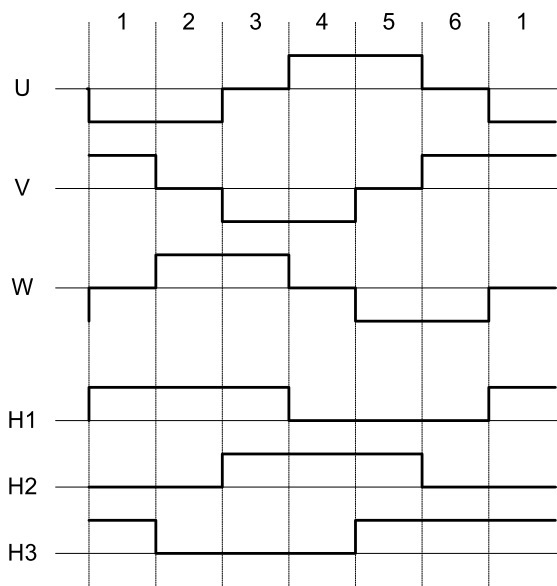
\includegraphics[scale=0.45]{Funktionstests/Bilder/ZeitlicheHallSensorAnsteuerung.jpg}
	\caption[Zeitliche Darstellung der Ansteuerung mit Hall-Sensoren]{Zeitliche Darstellung der Ansteuerung mit Hall-Sensoren \cite{AppNote:BrushlessuC}}
	\centering
    \label{abb:ZeitlicheAnsteuerungBrushlessMotor}
\end{wrapfigure}
Brushless-Motoren sind Synchron-Drehstrom-Motoren. Das heisst, sie werden mittels eines kontinuierlichen Drehfeld in Bewegung gesetzt. Dabei ist darauf zu achten, dass der Läufer dem Drehfeld synchron folgen kann, daher der Name. Falls der Läufer dem Drehfeld aus irgend einem Grund nicht folgen kann, so wird keine Spannung vom Rotor in die Statorwicklungen induziert, die der Erregerspannung entgegenwirkt. Daraus Folgt, dass ein immenser Strom fliesst, der nur von der Wicklungsimpedanz des Motors begrenzt wird.\\
Es gibt hauptsächlich zwei Methoden das Drehfeld zu regeln. Die eine und einfache Methode ist mittels drei Hallsensoren, die im Motor integriert sind. Dies macht den Motor aufwändiger und dementsprechend teurer. Die Regelung mit Hallsensoren ist verhältnismässig einfach, da je nach den Signalen die einzelnen Spulen direkt angesteuert werden kann. Der Zusammenhang zwischen der Ansteuerung und den Hall-Sensorsignalen ist in Abbildung \ref{abb:ZeitlicheAnsteuerungBrushlessMotor} ersichtlich. Dabei stehen $U$, $V$ und $W$ für die Phasenströme und $H_1$, $H_2$ und $H_3$ die entsprechenden Signale der Hallsensoren. Dieser Darstellung ist zu entnehmen, dass jedesmal wenn ein Hallsensor eine Änderung anzeigt, ein Nulldurchgang im entsprechenden Stromverlauf stattgefunden hat. Dies ist der Zeitpunkt, in dem die Kommutierung durchgeführt werden muss.
\\
\textbf{Aufbaubeschreibung}:
\begin{wrapfigure}{r}{0.55\textwidth}
	\includegraphics[scale=0.4]{Funktionstests/Bilder/MotoransteuerungSchema.jpg}
	\centering
	\caption{Schema des Brushless-Versuchsaufbaus}
\label{abb:MotoransteuerungSchema}
\end{wrapfigure}
Das Schema des gesamten Aufbaus des Tests ist in der Abbildung \ref{abb:MotoransteuerungSchema} abgebildet. Die 3-Phasen H-Brücke oben im grünen Rechteck wird direkt vom FPGA angesteuert. Die Hardware dieser Brücke ermöglicht eine voll galvanisch getrennte Ansteuerung mit 3.3V Logikpegeln. Diese Brücke wurde zur Verfügung gestellt und verwendet. Die Rekonstruktion der Hallsensoren-Signale findet im rot markierten Teil des Aufbaus statt. Dieser Part wurde auf einer Laborplatte aufgebaut und zusammen gelötet. Die so generierten Signale $U_{Hallsensor}$, $V_{Hallsensor}$, $W_{Hallsensor}$ werden einem FPGA geliefert. Anhand dieser Signale steuert dieses das FPGA die H-Brücken-Transistoren mittels der Signale $U_h$, $U_l$, $V_h$, $V_l$, $W_h$, $W_l$. Die im FPGA enthaltene Konfiguration sind simple AND-Verknüpfungen, die die anligenden Signale sehr schnell und effizient verarbeiten. Auf diese Weise ist es möglich, den Motor sehr schnell anzusteuern.\\
\\
In der Abbildung \ref{abb:MessplatzAufbau} ist der gesamte Aufbau abgebildet. Man beachte die markierten Felder. am unteren linken Rand ist der Motor befestigt. In der Mitte des Bildes ist die Hardware, mit der die Hallsensoren Signale rekonstruiert werden. Die generierten Signale werden dem FPGA in der unteren linken Ecke zugeführt. Diese Signale werden logisch verknüpft und danach werden die sechs Signale generiert um die H-Brücke in der oberen rechten Hälfte anzusteuern. Diese Wiederum treiben den Motor an.
\begin{figure}[h!]
%\vspace{-16pt}
	\includegraphics[scale=0.14]{Funktionstests/Bilder/MessplatzAufbau.jpg}
	\centering
	\caption{Testaufbau} 
\label{abb:MessplatzAufbau}
%\vspace{-10pt}
\end{figure}\\
Die im FPGA enthaltene Logik basiert auf der Wahrheitstabelle, die in Abbildung \ref{abb:WahrheitstabelleAnsteuerung} abgebildet ist.
\begin{figure}[h!]
\begin{tabular}{ccc||cc|cc|cc||c}
     $H_1$ & $H_2$ & $H_3$ & $U_h$ & $U_l$ & $V_h$ & $V_l$ & $W_h$ & $W_l$ & Illegal\\
\hline 0   &   0   &   0   &   0   &   0   &   0   &   0   &   0   &   0   &   1\\
       0   &   0   &   1   &   0   &   0   &   0   &   1   &   1   &   0   &   0\\
       0   &   1   &   0   &   0   &   1   &   1   &   0   &   0   &   0   &   0\\
       0   &   1   &   1   &   0   &   1   &   0   &   0   &   1   &   0   &   0\\
       1   &   0   &   0   &   1   &   1   &   0   &   0   &   1   &   0   &   0\\
       1   &   0   &   1   &   1   &   0   &   0   &   1   &   0   &   0   &   0\\
       1   &   1   &   0   &   0   &   0   &   1   &   0   &   0   &   1   &   0\\
       1   &   1   &   1   &   0   &   0   &   0   &   0   &   0   &   0   &   1\\
\end{tabular}
	\centering
	\caption{Wahrheitstabelle der Ansteuerung} 
\label{abb:WahrheitstabelleAnsteuerung}
\end{figure}\\
Die Tabelle kann pro Signal zu folgenden logischen Verknüpfung vereinfacht werden.\\
\begin{tabular}{ccc}
$U_h = H_1 \wedge \bar{H_2}$ & $V_h = H_2 \wedge \bar{H_3}$ & $W_h = \bar{H_1} \wedge H_3$\\
$U_l = \bar{H_1} \wedge H_2$ & $V_l = \bar{H_2} \wedge H_3$ & $W_l = H_1 \wedge \bar{H_3}$
\end{tabular}

    \newpage
    \ifSTANDALONE
\section{Prinziptest}
\fi
\ifEMBED
\subsubsection{Aufbaubeschreibung}
    \BLDCcollab \\
\fi
\ifEMBED
    \begin{wrapfigure}{r}{0.55\textwidth}
       	\includegraphics[scale=0.4]{\EtPath/Bilder/MotoransteuerungSchema.jpg}
       	\centering
       	\caption{Schema des Brushless-Versuchsaufbaus}
        \label{abb:MotoransteuerungSchema}
    \end{wrapfigure}
\fi
    Das Schema des Gesamtaufbaus des Tests ist in der Abbildung 
    \ref{abb:MotoransteuerungSchema} ersichtlich. Die 3-Phasen H-Brücke 
    im oberen grünen Rechteck wird direkt vom FPGA\footnote{\textbf{F}ield-\textbf{P}rogrammable \textbf{G}ate \textbf{A}rray} angesteuert. Die Hardware 
    dieser Brücke ermöglicht eine voll galvanisch getrennte Ansteuerung 
    mit $3.3 V$ Logikpegeln. Diese Brücke wurde zur Verfügung gestellt und direkt
    verwendet. Die Rekonstruktion der Hallsensoren-Signale findet im rot 
    markierten Teil des Aufbaus statt. Dieser Part wurde auf einer 
    Laborplatte aufgebaut und gelötet. Die so generierten Signale 
    $U_{Hallsensor}$, $V_{Hallsensor}$, $W_{Hallsensor}$ werden einem FPGA 
    geliefert. Anhand dieser Signale steuert das FPGA die 
    H-Brücken-Transistoren mit den Signalen $U_h$, $U_l$, $V_h$, $V_l$, 
    $W_h$, $W_l$. Die im FPGA enthaltene Konfiguration besteht aus simplen 
    AND-Verknüpfungen, die die anliegenden Signale sehr schnell und 
    effizient verarbeiten können. Auf diese Weise ist es möglich, den Motor sehr 
    schnell anzusteuern.
    \ifSTANDALONE
    \begin{figure}[h!]
    	\includegraphics[scale=0.4]{\EtPath/Bilder/MotoransteuerungSchema.jpg}
       	\centering
       	\caption{Schema des Brushless-Versuchsaufbaus}
        \label{abb:MotoransteuerungSchema}
    \end{figure}
    \fi
    In der Abbildung \ref{abb:MessplatzAufbau} ist der gesamte Aufbau 
    abgebildet. Man beachte die markierten Felder. Am linken unteren Rand 
    ist der Motor befestigt. In der Mitte des Bildes ist die Hardware zur Rekonstruktion der Hallsensoren-Signale.
    Die generierten Signale werden dem FPGA in der unteren linken Ecke zugeführt. Diese 
    Signale werden logisch verknüpft und danach die sechs Signale 
    generiert, um die H-Brücke in der rechten oberen Hälfte anzusteuern. 
    Die H-Brücken wiederum treiben den Motor an.
    \begin{figure}[h!]
    %\vspace{-16pt}
       	\includegraphics[width=0.9\textwidth]{\EtPath/Bilder/MessplatzAufbau.jpg}
       	\centering
       	\caption{Testaufbau} 
        \label{abb:MessplatzAufbau}
    %\vspace{-10pt}
    \end{figure}
    Die im FPGA enthaltene Logik basiert auf der Wahrheitstabelle, die in 
    Tabelle \ref{abb:WahrheitstabelleAnsteuerung} abgebildet ist.

\ifSTANDALONE
\subsection{Messmittel}
\fi
\ifEMBED
%\newpage
\subsubsection{Messmittel}
\fi
    \begin{table}[h!]
        \centering
        \begin{tabular}{lll}
            \rowcolor{gray}
            Gerät &
                Typ &
                Nummer \\
            Speisegerät & 
                Rohde \& Schwarz NGSM 32/10 &
                Inv.-Nr. 009 \\
            Oszilloskop &
                Agilent MSO6052A &
                Inv.-Nr. 44; S/N: MY44001903 \\
            Mainframe &
                Hameg HM8001-2 &
                SN: 059520046 \\
            Speisegerät &
                Hameg HM8040-3 &
                SN: 015405014 \\
            Pulsgenerator &
                Hameg HM8035 &
                Inv.-Nr. 44 \\
        \end{tabular}
        \caption{Messmittel des Versuchsaufbaus}
    \end{table}

\ifSTANDALONE
\subsection{Resultat}
\label{chap:VersuchsResultat}
\fi
\ifEMBED
\subsubsection{Resultat}
\label{chap:VersuchsResultat}
\fi
Mit dem beschriebenen Aufbau konnte ein BLDC-Motor erfolgreich angesteuert werden. Wie in Abbildung
 \ref{abb:MessplatzAufbau} am linken unteren Rand zu erkennen ist, ist an der Motorwelle eine 
 Aluminiumplatte montiert. Mit dieser und eines Magneten konnte der Motor mittels einer Wirbelstrombremse 
 belastet werden. Auf diese weise konnte rund $120 W$ elektrische Leistung umgesetzt werden. Dabei 
 stellte sich heraus, dass die PWM nachgeregelt werden muss, wenn eine Last getrieben wird. Weiter 
 bietet der Aufbau, wie er getestet wurde keine Möglichkeit den Motor ohne äussere Manipulation zu 
 starten.\\
\\
Diese beiden Tatsachen sprechen dafür, dass das Prinzip grundsätzlich funktioniert. Für die Realisierung 
würde sich ein eigenes Board anbieten, auf dem ein eigener Controller die Regelung und die Zwangskommutierung beim Starten des Motors übernimmt.
    \ifSTANDALONE
\section{Fallback}
\fi
\ifEMBED
\subsubsection{Fallback}
\fi
Ist der Einsatz des vorgesehenen BLDC-Treibers nicht möglich, so muss eine
alternative Ansteuerung erfolgen. Eine solche kann mit einer handelsüblichen
Steuerungen aus dem Modellbau erfolgen. Eine solche BLDC-Steuerung ist per
PWM angesteuert, wobei die im Modellbau üblichen Signale gelten, wie in der
Abbildung \ref{fig:rc-pwm} dargestellt.

\begin{figure}[h!]
	\centering
	\begin{tikzpicture}
		% Achsen
		\draw[->] (-0.25,0) -- (10,0) node[anchor=north] {$t$};
		\draw[->] (0,-0.25) -- (0,3) node[anchor=west] {$u$};
		% Signal
		\draw[-,red,thick] (0,0) -- (1,0) -- (1,2) -- (2,2) -- 
			(2,0) -- (7,0) -- (7,2) -- (8,2) -- (8,0) -- (9,0);
		% Zeiten
		\draw[<->] (1,1.5) -- (7,1.5) node[midway, above] {$T=20$ms};
		\draw[<->] (1,0.5) -- (2,0.5) node[right] {$1$ms$<t_{ON}<2$ms};
	\end{tikzpicture}
	\caption{Signalverlauf eines typischen Modellbau-PWM Signals}
	\label{fig:rc-pwm}
\end{figure}

Der Einsatz von Modellbausteuerungen für BLDC-Motoren erfordert ein
Feedback der Drehzahl, da diese lediglich eine Steuerung darstellen. Die
Drehzahlregelung muss über eine externe Einheit erfolgen, beispielsweise einen
Mikrocontroller. Solche BLDC-Steuerungen werden im Modellbau typischerweise als
\emph{Regler} vertrieben und sind auch für hohe Leistungen durchaus preiswert.

\ifSTANDALONE
\subsection{Konzeptbeschreibung}
\fi
\ifEMBED
\paragraph{Konzeptbeschreibung\\}
\fi
Um eine Regelung der Drehzahl des BLDC-Motors zu ermöglichen, bedarf es eines
Feebacks, welches die Drehzahl wiedergibt. Dies ist mit einem
Hall-Effekt-Schalter zu realisieren. Dieser reagiert auf die Magnetfelder,
welche durch Magnete auf dem Rotationskörper gegeben sind. Aus solch einem
Aufbau resultiert ein Feedback, welches mit Impulsen einen Segmentdurchlauf
des Rotationskörpers wiedergibt, wie in Abbildung \ref{fig:fallback-sketch}
dargestellt.
\begin{figure}[h!]
	\centering
	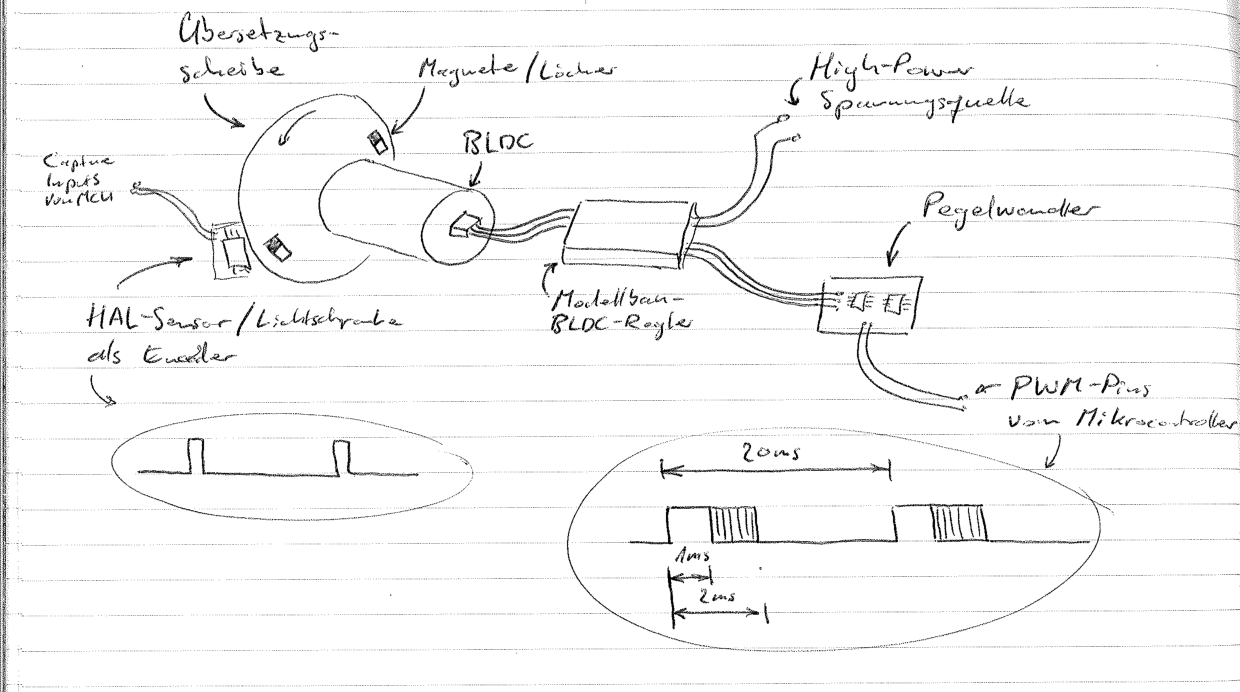
\includegraphics[width=0.8\textwidth]{\EtPath/Bilder/fallback_sketch_1.pdf}
	\caption{Erste Skizze des Fallback-Konzepts}
	\label{fig:fallback-sketch}
\end{figure}
Dieses Feedback wird mittels eines Mikrocontrollers ausgewertet und regelt
damit den Input der Steuerung mit dem PWM-Signal beziehungsweise der Impulsdauer.
Das Einlesen einer Flanke, die Zeitmessung bis zur nächsten Flanke und die
Stellung eines PWM-Signals, sind Tasks welche übliche Mikrocontroller direkt
durch ihre Peripherie-Module ausführen können. Dies ermöglicht eine einfache
Adaption in ein bestehendes Modell, denn es werden lediglich zwei Timer-IO
für diesen Fallback verwendet. Je nach Mikrocontroller ist ein Pegelwandler
für die PWM-Signale notwendig.

    \ifSTANDALONE
\section{Encoder \& Drehzahlgeber}
\fi
\ifEMBED
\subsubsection{Encoder \& Drehzahlgeber}
\fi

Die vorgesehenen Motorfunktionen verlangen lediglich beim Brushlessmotor
nach einem Feedback über die Rotation des Motors, da der Schrittmotor
definiert und fein granuliert betrieben wird. Der Gleichstrommotor stellt
keinerlei Ansprüche, weder an die Drehzahl, noch an die Position.

Encoder sind relativ teuer und der Einsatz des Brushlessmotors verlangt
lediglich nach einem Feedback zur Rotation beziehungsweise Winkelgeschwindigkeit.
Die absolute oder relative Position ist für die Anwendung nicht von
Bedeutung. Somit lässt sich ein einfaches Feedback vorsehen, für die
Regelung der Drehzahl mit optischen oder magnetischen Elementen.
\ifSTANDALONE
\begin{figure}[h!]
	\centering
	\begin{tikzpicture}
	% Koordinaten
	\draw[->] (-0.5, 0) -- (8, 0) node[anchor=north] {$t$};
	\draw[->] (0, -1.5) -- (0, 3) node[anchor=east] {$u,\varphi$};
	% Rotation
	\draw[blue] (0,0) sin (1,1) cos (2,0) sin (3,-1) cos (4,0)
	sin (5,1) cos (6,0) sin (7,-1)
	node[right] {$\varphi$};
	% Signal
	\draw[-, thick, red]
	(0,0) -- (0.8,0) -- (0.8,2) -- (1.2,2) -- (1.2,0) -- 
	(4.8,0) -- (4.8,2) -- (5.2,2) -- (5.2,0) -- (7.5,0);
	% Messung
	\draw[<->] (0.8,1.5) -- (4.8,1.5) node[midway, above] {$t_{r}$};
	\end{tikzpicture}
	\caption{Vereinfachtes Puls-Feedback eines Hall-Effekt-Schalters}
	\label{fig:hall-effekt-schalter}
\end{figure}
\fi
\ifEMBED
\begin{figure}[h!]
	\centering
	\begin{tikzpicture}
	% Koordinaten
	\draw[->] (-0.5, 0) -- (8, 0) node[anchor=north] {$t$};
	\draw[->] (0, -1.5) -- (0, 3) node[anchor=east] {$u,\varphi$};
	% Rotation
	\draw[blue] (0,0) sin (1,1) cos (2,0) sin (3,-1) cos (4,0)
	sin (5,1) cos (6,0) sin (7,-1)
	node[right] {$\varphi$};
	% Signal
	\draw[-, thick, red]
	(0,0) -- (0.8,0) -- (0.8,2) -- (1.2,2) -- (1.2,0) -- 
	(4.8,0) -- (4.8,2) -- (5.2,2) -- (5.2,0) -- (7.5,0);
	% Messung
	\draw[<->] (0.8,1.5) -- (4.8,1.5) node[midway, above] {$t_{r}$};
	\end{tikzpicture}
	\caption{Vereinfachtes Puls-Feedback eines Hall-Effekt-Schalters}
	\label{fig:hall-effekt-schalter}
\end{figure}
\fi
Als optisches Messinstrument kann eine Lichtschranke mit 
Reflexionsstreifen oder Löchern eingesetzt werden. Diese verlangen
nur nach einer geringfügigen Modifikation des rotierenden Körpers und
sind relativ günstig. Optische Messtechnik hat den Nachteil, das
Störungen relativ leicht in die Messung einfliessen können, was fatale
Folgen für die Regelung hat. Magnetische Messinstrumente sind gegenüber
Störungen deutlich resistenter, da hierfür starke Magnetfelder benötigt
werden, welche so nicht einfach auftreten. Der Einsatz einer solchen Messtechnik
verlangt jedoch nach einer Modifikation der Mechanik, da Magnete in den
rotierenden Körper eingebaut werden müssen. Dies birgt ein gewisses
Risiko für mechanische Unwucht des Rotationskörpers.

\ifSTANDALONE
\subsection{Magnetischer Drehzahlgeber}
\fi
\ifEMBED
\paragraph{Magnetischer Drehzahlgeber\\}
\fi
Um einen eigenen magnetischen Drehzahlgeber zu erstellen wird ein
sogenannter Hall-Effekt-Schalter eingesetzt. Dieser reagiert mit seinem Ausgang
auf ein auftretendes Magnetfeld. Das Gegenstück zum Hall-Effekt-Schalter
ist ein Magnet, welcher in das rotierende Objekt eingebaut wird. Aus 
mechanischen Gründen, wie etwa der Unwucht, werden typischerweise 2 Magnete
oder ein Vielfaches davon in den rotierenden Körper eingebaut.

Bei der Rotation des Körpers entstehen durch das Passieren der Magnete
am Hall-Effekt-Schalter Impulse. Aus diesen Impulsen lässt sich mit einer
Zeitmessung direkt die Drehzahl bestimmen. Die Abbildung 
\ref{fig:hall-effekt-schalter} illustriert das Prinzip anhand eines
Beispiels mit einem Magneten am Rotationskörper.
%
\ifSTANDALONE
\begin{figure}[h!]
	\centering
	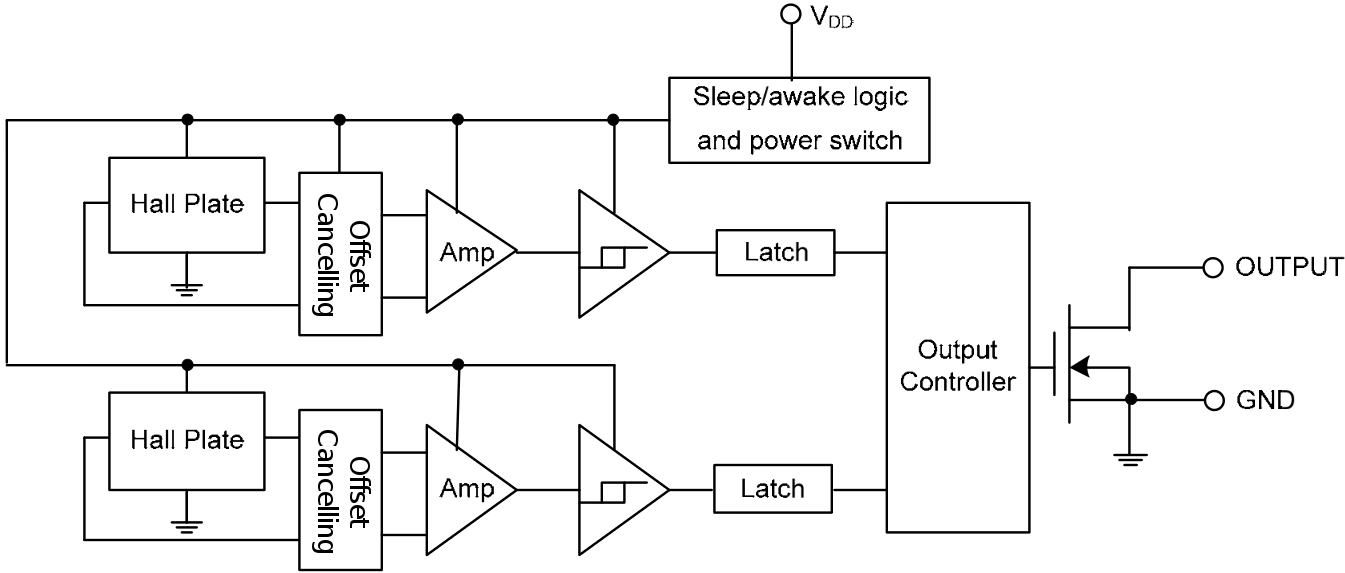
\includegraphics[width=0.75\textwidth]{\EtPath/Bilder/AH180N_functional.png}
	\caption{Funktionelles Blockschaltbild des Hall-Effekt-Schalters AH180N}
	\label{fig:AH180N_functional}
\end{figure}
\fi
%
\ifEMBED
\begin{figure}[h!]
	\centering
	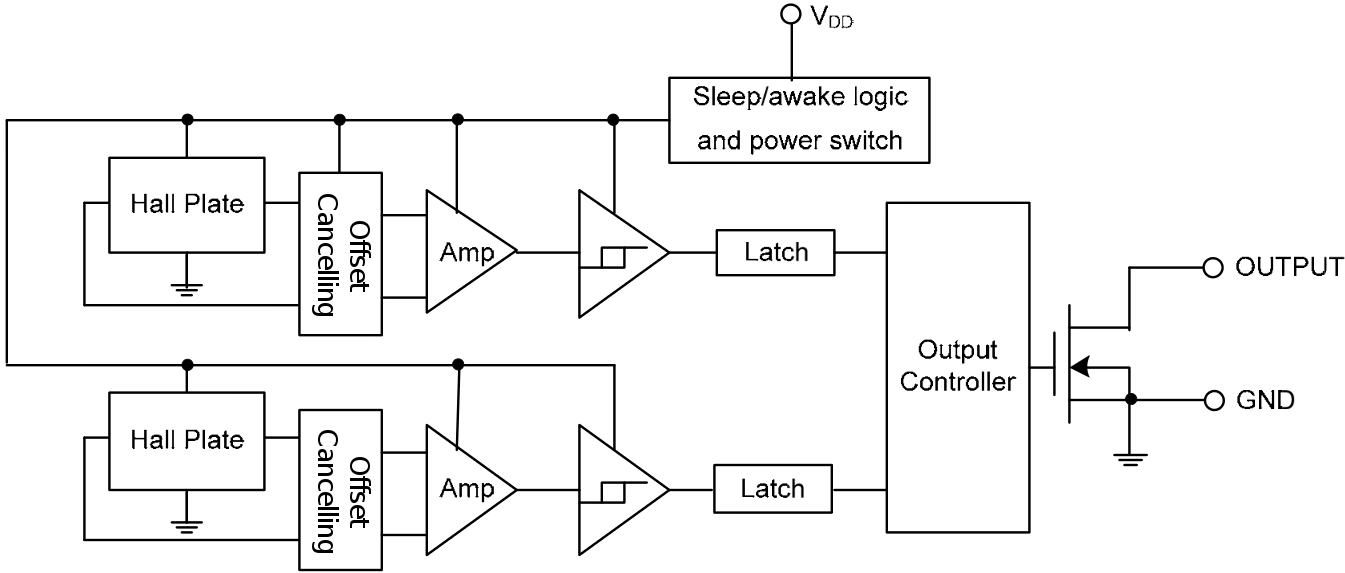
\includegraphics[width=0.75\textwidth]{\EtPath/Bilder/AH180N_functional.png}
	\caption{Funktionelles Blockschaltbild des Hall-Effekt-Schalters AH180N}
	\label{fig:AH180N_functional}
\end{figure}
\fi
%
Ein solches Verfahren lohnt sich bei schnellen Winkelgeschwindigkeiten
und ist für diesen Anwendungsfall sehr effizient. Zugehörige
Hall-Effekt-Schalter lassen sich einfach montieren und sind gegen Störungen
sehr robust. Ein mögliches Modell für einen Hall-Effekt-Schalter ist der
AH180N. Dieser bietet einen Open-Drain Ausgang, welcher somit logische Pegel
liefert (siehe Abbildung \ref{fig:AH180N_functional}). Interessant ist diese
Art von Drehzahl-Geber insbesondere durch ihren geringen Preis, denn solche
Hall-Effekt-Schalter, wie der AH180N, befinden sich im Preissegment von 
unter einem Franken.
    \subsection{Acrylglas}
\begin{tabular}{p{3.6cm}p{9.4cm}}
	\rule{0pt}{11pt}\textit{Typ}              & Lagerung und Bohrung in Acrylglas  \\ 
	\rule{0pt}{11pt}\textit{Datum}:           & 21.11.2014   \\
	\rule{0pt}{11pt}\textit{Ort}:             & Labor HSLU \\
	\rule{0pt}{11pt}\textit{Tester}:          & Matteo, Pascal\\
	\rule{0pt}{11pt}\textit{Ziel des Testes}: & Lassen sich Wälzlager in Acrylglas (PMMA) einpressen und halten sie den herrschenden Druck stand? Verhalten, Möglichkeiten von Bohrungen in $5 mm$ Acrylglas.   \\
	\rule{0pt}{11pt}\textit{Fazit / Verbesserungs-\newline vorschlag}: & Beim ersten Versuch sind Spannungsrisse aufgetreten (siehe Pfeil in Abbildung \ref{abb:LagerPlexiglas}). 
	Um dem entgegenzuwirken, wurde in einem zweiten Versuch die $16 mm$ Bohrung mit 
	Schleifpapier geringfügig vergrössert, damit sich das Lager leichter einpressen lässt. 
	Die Kräfte, die durch das Lager aufgenommen werden können, sind nun zwar 
	geringer, allerdings für den geplanten Einsatzbereich immer noch genügend. 
	Durch diese Methode treten auch keine Spannungsrisse mehr auf. \newline	
	Die Bohrung sollte mit einem sehr scharfen Bohrer mit stumpfem Winkel 
	gemacht werden. Weiter sollte sie gekühlt werden, um ein Durchschmelzen 
	durch die sehr dünne, noch verbleibende Restwandstärke, zu verhindern.  \\
	\rule{0pt}{11pt}\textit{Ziel erreicht}:& Ja\\
\end{tabular}
\begin{figure}[h!]
	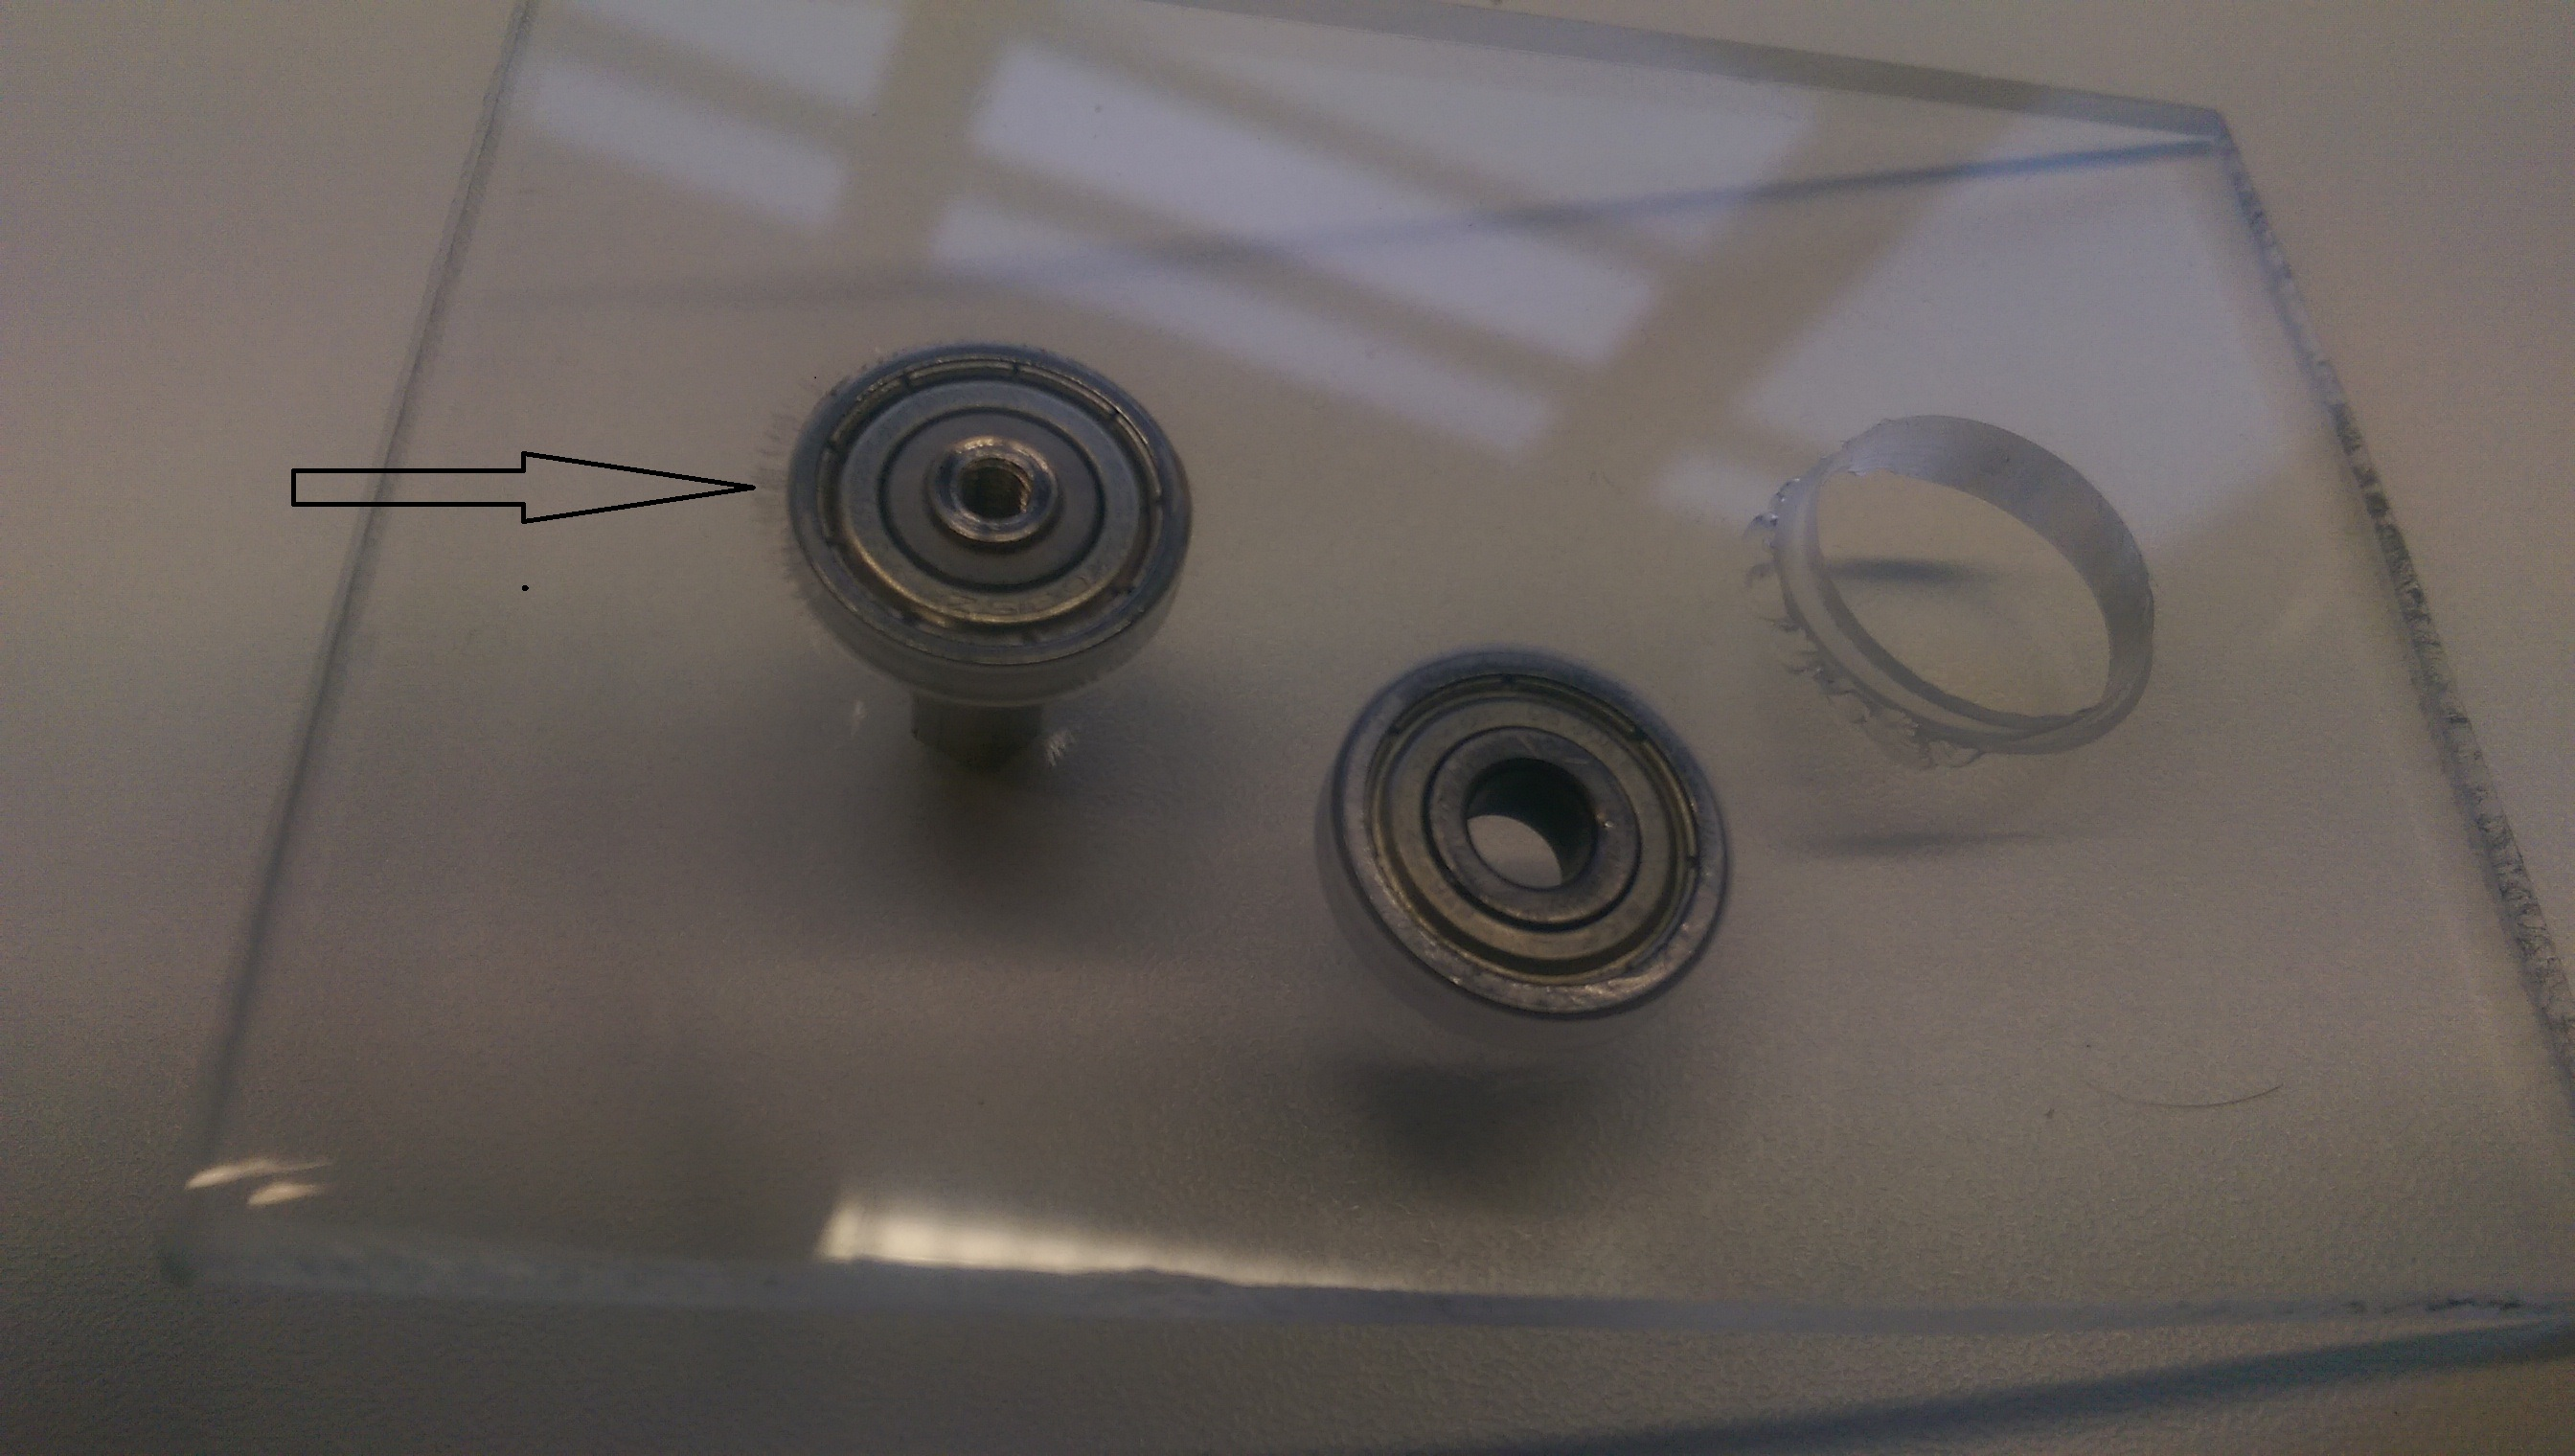
\includegraphics[width=0.9\textwidth,clip,trim=10cm 15cm 40cm 6cm]
	{Funktionstests/Bilder/LagerPlexiglas.jpg}
	\centering
	\caption{Spannungsrisse in Acrylglas-Funktionsmuster} 
	\label{abb:LagerPlexiglas}
\end{figure}
    \subsection{Ballmaschine}
\begin{tabular}{p{3.6cm}p{9.4cm}}
\rule{0pt}{11pt}\textit{Typ}              & Ballmaschine \\ 
\rule{0pt}{11pt}\textit{Datum}:           & 18.10.2014   \\
\rule{0pt}{11pt}\textit{Ort}:             & Labor HSLU \\
\rule{0pt}{11pt}\textit{Tester}:          & Gruppe 32 \\
\rule{0pt}{11pt}\textit{Ziel des Testes}: & Das Ziel dieses Testes bestand darin: Den gebauten Prototyp (Ballmaschine) auf die Genauigkeit und Wurfweite zu testen, weitere Erkenntnisse über die Drehzahl der Räder zu eruieren und die erforderliche Stromstärke unter realen Bedingungen testen.  \\
\rule{0pt}{11pt}\textit{Fazit / Verbesserungs-\newline vorschlag}: & Die Wurfmaschine kann mit einigen Verbesserungen sehr gute und genaue „Schüsse“ erzielen. Zu verbessern sind:
\begin{itemize}
    \item Stabilere Achsen
    \item genauere und gleichmässige Zuführung der Bälle.
    \item einstellbares Grundgerüst
\end{itemize}\\
\textit{Ziel erreicht}:& Ja\\
\end{tabular}

    \subsection{Pneumatikzylinder}

\begin{tabular}{p{3.6cm}p{\textwidth-3.6cm-0.7cm}}
\rule{0pt}{11pt}\textit{Typ}              & Ballmaschine \\ 
\rule{0pt}{11pt}\textit{Datum}:           & 08.10.2014   \\
\rule{0pt}{11pt}\textit{Ort}:             & Bachmann Engineering AG (Zofingen) \\
\rule{0pt}{11pt}\textit{Tester}:          & Gruppe 32\\
\rule{0pt}{11pt}\textit{Ziel des Testes}: & Das Ziel dieses Testes bestand darin, den gebauten Prototyp auf die Wurfwiederholgenauigkeit zu testen. \\
\rule{0pt}{11pt}\textit{Fazit / Verbesserungs-\newline vorschlag}: & Ein Pneumatikzylinder arbeitet sehr zielgenau und schnell. Falls dieses Verfahren in die engere Auswahl kommt, müssen die Parameter wie Beschleunigung, Abschussgeschwindigkeit und Druck berechnet werden.\\ 
\end{tabular}

\begin{figure}[h!]
	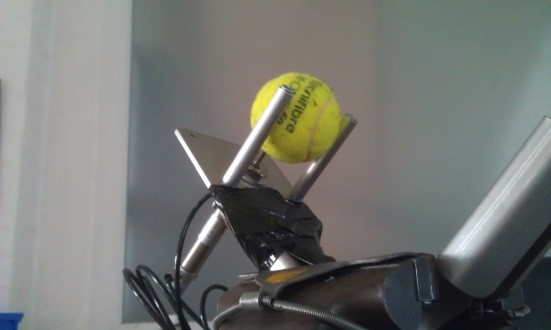
\includegraphics[width=0.8\textwidth]{Funktionstests/Bilder/PneumatikzylinderBild.jpg}
	\centering
	\caption{Funktionsmuster Pneumatikzylinder} 
\label{abb:PneumatikzylinderBild}
\end{figure}
    \subsection{Ballmaschine (Eruieren der Nenndrehzahl)}

\begin{tabular}{p{3.6cm}p{\textwidth-3.6cm-0.7cm}}
\rule{0pt}{11pt}\textit{Typ}              & Ballmaschine \\ 
\rule{0pt}{11pt}\textit{Datum}:           & 06.11.2014   \\
\rule{0pt}{11pt}\textit{Ort}:             & Labor HSLU \\
\rule{0pt}{11pt}\textit{Tester}:          & Matteo, Yves, Pascal\\
\rule{0pt}{11pt}\textit{Ziel des Testes}: & Bestimmung der Nenndrehzahl der 
Schwungräder sowie die Optimierung des Wurfwinkel.  \\
\rule{0pt}{11pt}\textit{Aufbau / Ablauf}: & In diesem Test wurde die Ballmaschine 
aus dem gleichnamigen Test mit demselben Aufbau verwendet. Die Drehzahl der beiden DC-Motoren
wird mittels der Labornetzgeräte eingestellt. Die Messung der Drehzahl erfolgt über ein berührendes 
Drehzahlmessgerät, das aus dem Physikbestand der Hochschule Luzern ausgeliehen wurde.\\
\rule{0pt}{11pt}\textit{Fazit / Verbesserungs-\newline vorschlag}: & Die Ballzuführung 
muss automatisiert und gleichbleibend sein, damit genaue Aussagen über die Drehzahl 
und dadurch die Wurfweite gemacht werden können. Weiter ist festgestellt worden, dass 
es eine markanten Unterschiedliche zwischen unterschiedlichen Tennisballmarken gibt. 
Diese variieren im Durchmesser und Härte. Dadurch variiert auch die Wurfweite. Für 
die nächsten Test, müssen fünf für den Wettkampf zugelassene Bälle verwendet werden. 
Die Drehzahl der Schwungräder bei einem Abstand von $1.8 m$ beträgt rund 
$6000\frac{U}{min}$. Diese Drehzahl wird sich noch ändern, wenn andere Schwungräder 
eingesetzt werden.
\end{tabular}
%\begin{figure}[h!]
%	\includegraphics[width=0.7\textwidth,clip,trim=0mm 10cm 0mm 12cm]
%	{Funktionstests/Bilder/Ballmaschine_Drehzahl1.jpg}
%	\centering
%	\caption{Funktionsmuster Ballmaschine} 
%\label{abb:Ballmaschine_Drehzahl}
%\end{figure}
    \subsection{Acrylglas}
\begin{tabular}{p{3.6cm}p{9.4cm}}
	\rule{0pt}{11pt}\textit{Typ}              & Lagerung und Bohrung in Acrylglas  \\ 
	\rule{0pt}{11pt}\textit{Datum}:           & 21.11.2014   \\
	\rule{0pt}{11pt}\textit{Ort}:             & Labor HSLU \\
	\rule{0pt}{11pt}\textit{Tester}:          & Matteo, Pascal\\
	\rule{0pt}{11pt}\textit{Ziel des Testes}: & Lassen sich Wälzlager in Acrylglas (PMMA) einpressen und halten sie den herrschenden Druck stand? Verhalten, Möglichkeiten von Bohrungen in $5 mm$ Acrylglas.   \\
	\rule{0pt}{11pt}\textit{Fazit / Verbesserungs-\newline vorschlag}: & Beim ersten Versuch sind Spannungsrisse aufgetreten (siehe Pfeil in Abbildung \ref{abb:LagerPlexiglas}). 
	Um dem entgegenzuwirken, wurde in einem zweiten Versuch die $16 mm$ Bohrung mit 
	Schleifpapier geringfügig vergrössert, damit sich das Lager leichter einpressen lässt. 
	Die Kräfte, die durch das Lager aufgenommen werden können, sind nun zwar 
	geringer, allerdings für den geplanten Einsatzbereich immer noch genügend. 
	Durch diese Methode treten auch keine Spannungsrisse mehr auf. \newline	
	Die Bohrung sollte mit einem sehr scharfen Bohrer mit stumpfem Winkel 
	gemacht werden. Weiter sollte sie gekühlt werden, um ein Durchschmelzen 
	durch die sehr dünne, noch verbleibende Restwandstärke, zu verhindern.  \\
	\rule{0pt}{11pt}\textit{Ziel erreicht}:& Ja\\
\end{tabular}
\begin{figure}[h!]
	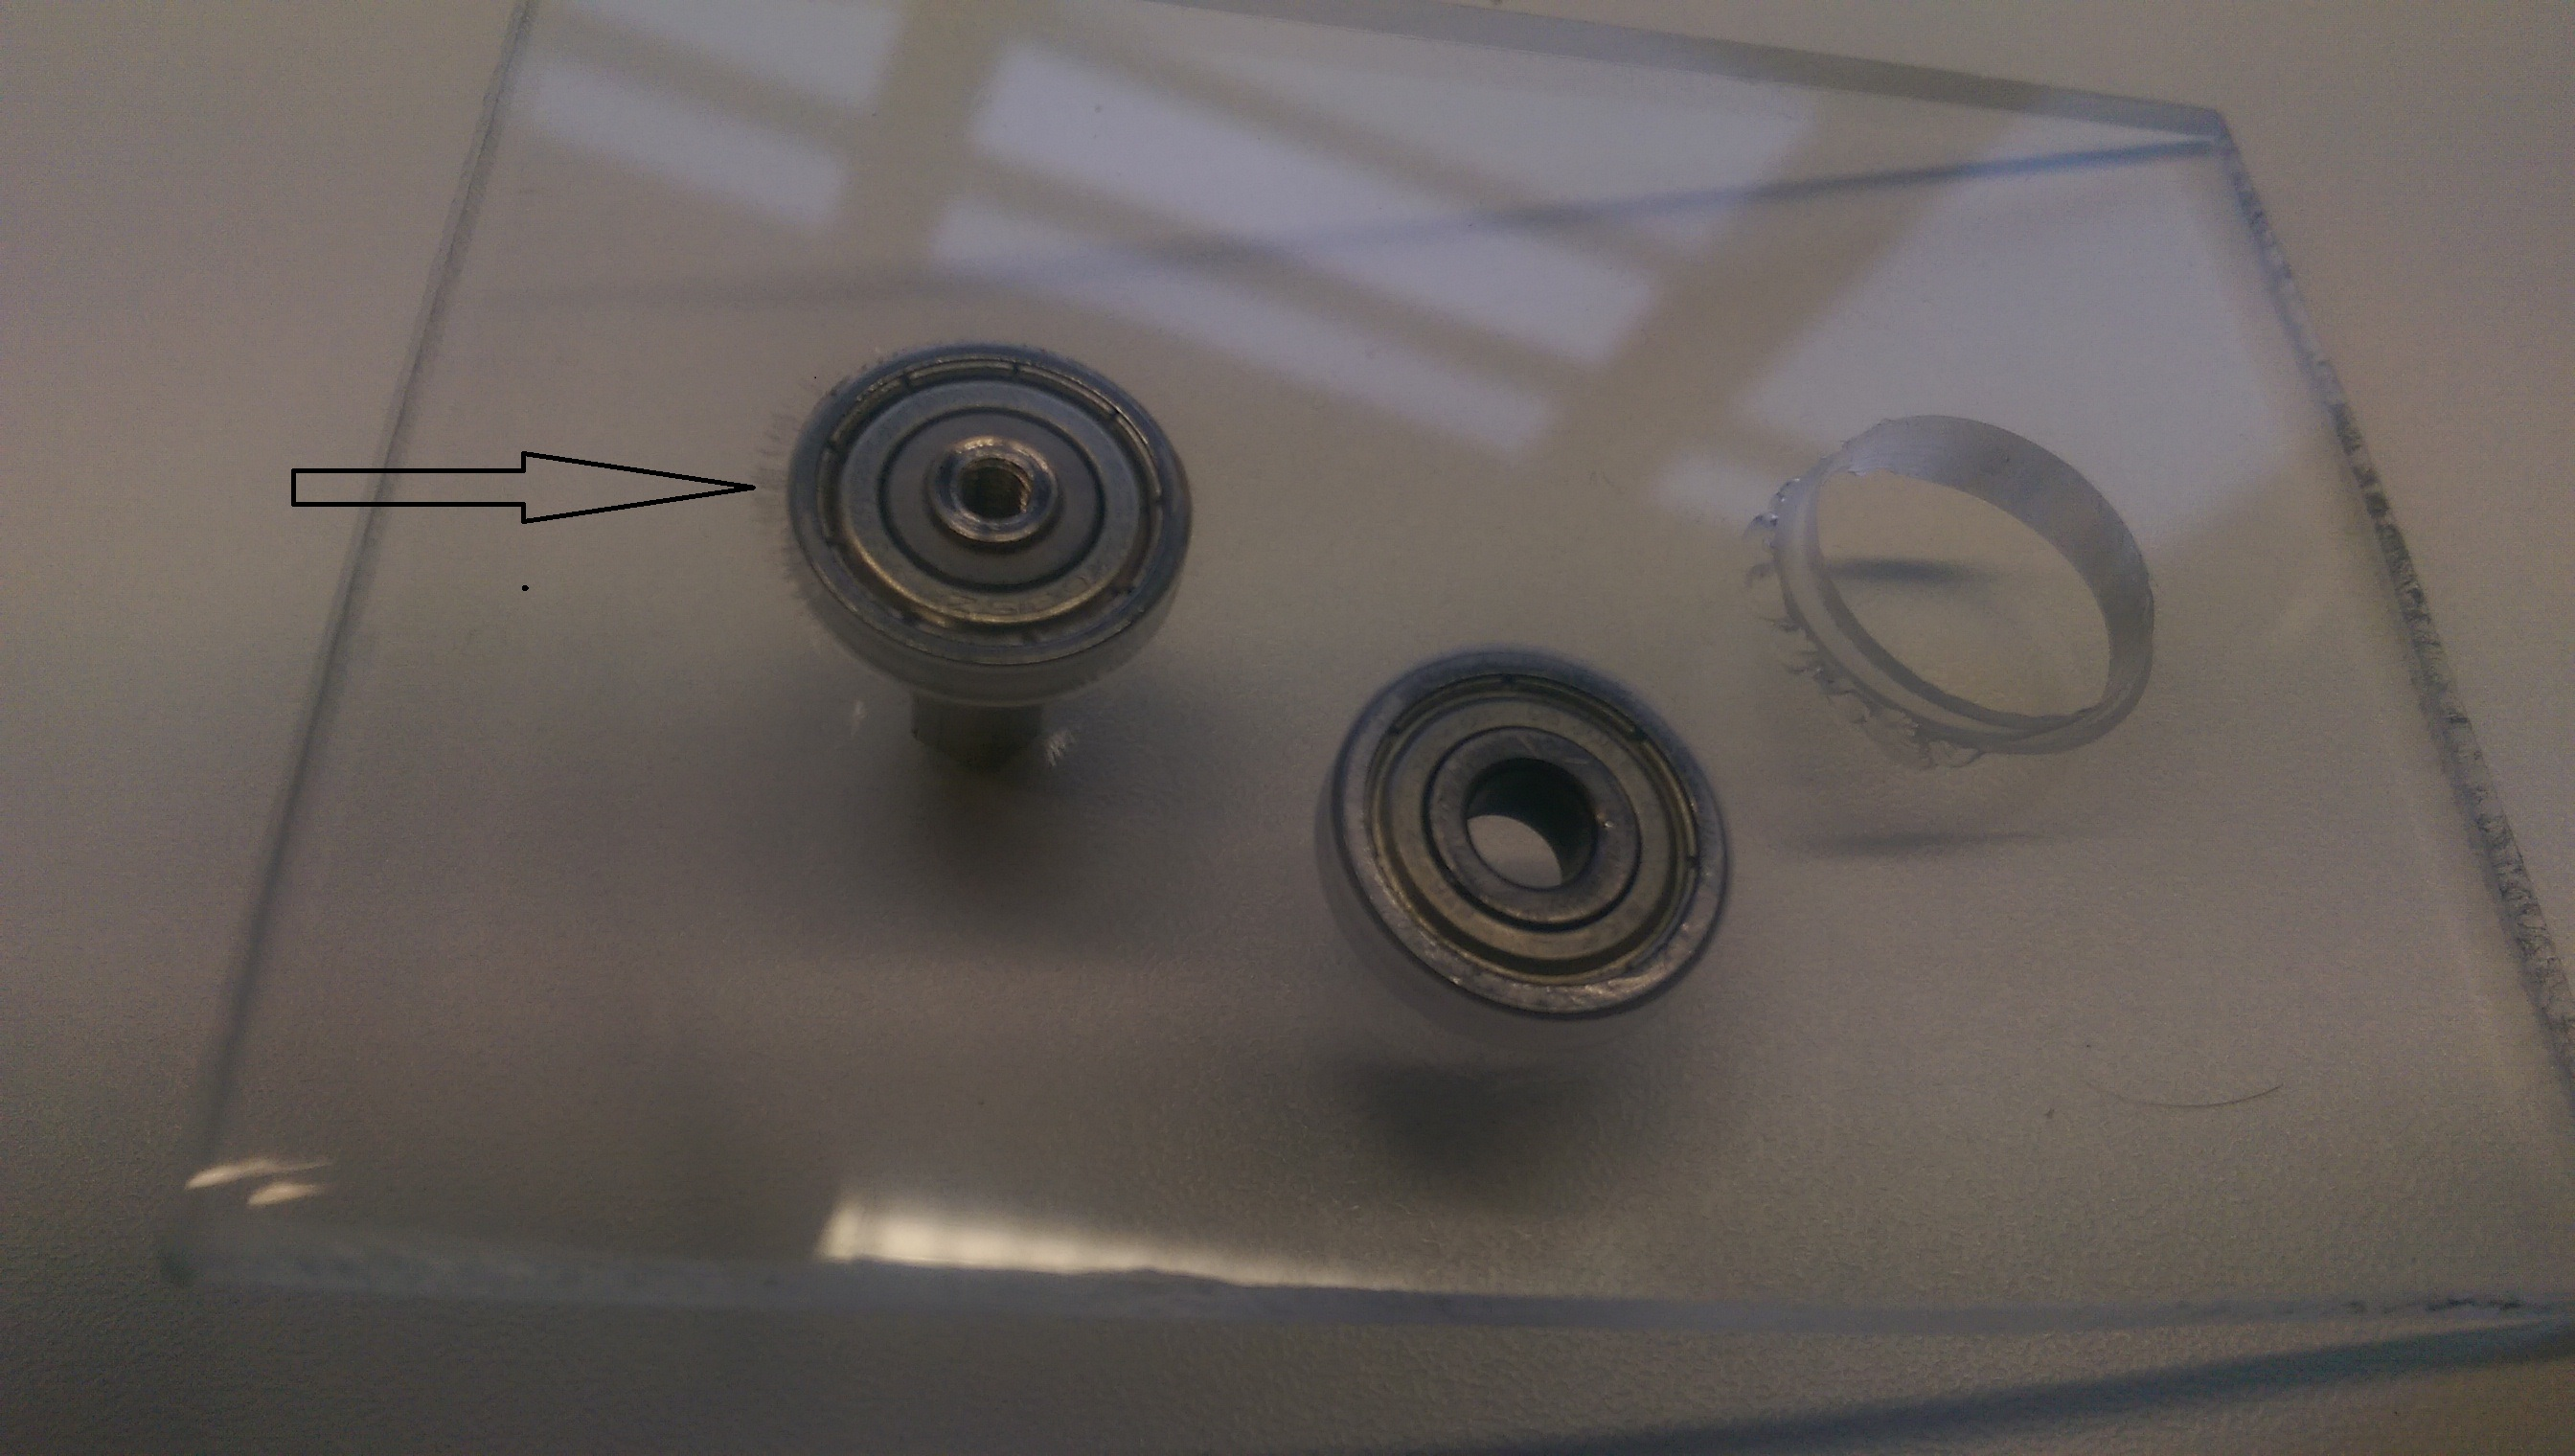
\includegraphics[width=0.9\textwidth,clip,trim=10cm 15cm 40cm 6cm]
	{Funktionstests/Bilder/LagerPlexiglas.jpg}
	\centering
	\caption{Spannungsrisse in Acrylglas-Funktionsmuster} 
	\label{abb:LagerPlexiglas}
\end{figure}
    \newpage
    \subsection{Brushless-Motor-Test}
    \subsubsection{Brushless Motoransteuerung}
\textbf{Theorie der Ansteuerung}:\\
\begin{wrapfigure}{r}{0.50\textwidth}
	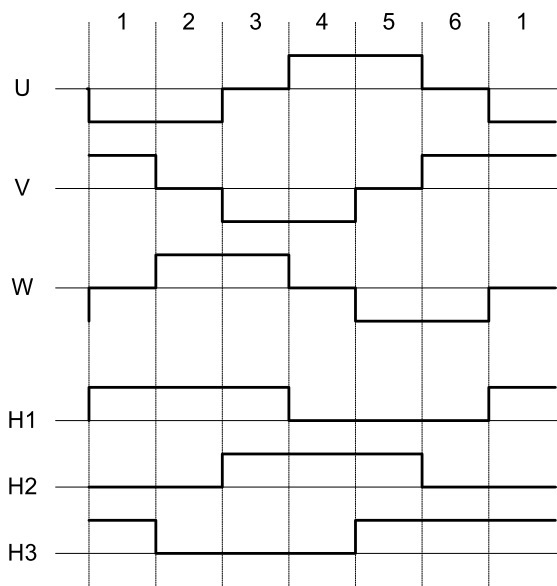
\includegraphics[scale=0.45]{Funktionstests/Bilder/ZeitlicheHallSensorAnsteuerung.jpg}
	\caption[Zeitliche Darstellung der Ansteuerung mit Hall-Sensoren]{Zeitliche Darstellung der Ansteuerung mit Hall-Sensoren \cite{AppNote:BrushlessuC}}
	\centering
    \label{abb:ZeitlicheAnsteuerungBrushlessMotor}
\end{wrapfigure}
Brushless-Motoren sind Synchron-Drehstrom-Motoren. Das heisst, sie werden mittels eines kontinuierlichen Drehfeld in Bewegung gesetzt. Dabei ist darauf zu achten, dass der Läufer dem Drehfeld synchron folgen kann, daher der Name. Falls der Läufer dem Drehfeld aus irgend einem Grund nicht folgen kann, so wird keine Spannung vom Rotor in die Statorwicklungen induziert, die der Erregerspannung entgegenwirkt. Daraus Folgt, dass ein immenser Strom fliesst, der nur von der Wicklungsimpedanz des Motors begrenzt wird.\\
Es gibt hauptsächlich zwei Methoden das Drehfeld zu regeln. Die eine und einfache Methode ist mittels drei Hallsensoren, die im Motor integriert sind. Dies macht den Motor aufwändiger und dementsprechend teurer. Die Regelung mit Hallsensoren ist verhältnismässig einfach, da je nach den Signalen die einzelnen Spulen direkt angesteuert werden kann. Der Zusammenhang zwischen der Ansteuerung und den Hall-Sensorsignalen ist in Abbildung \ref{abb:ZeitlicheAnsteuerungBrushlessMotor} ersichtlich. Dabei stehen $U$, $V$ und $W$ für die Phasenströme und $H_1$, $H_2$ und $H_3$ die entsprechenden Signale der Hallsensoren. Dieser Darstellung ist zu entnehmen, dass jedesmal wenn ein Hallsensor eine Änderung anzeigt, ein Nulldurchgang im entsprechenden Stromverlauf stattgefunden hat. Dies ist der Zeitpunkt, in dem die Kommutierung durchgeführt werden muss.
\\
\textbf{Aufbaubeschreibung}:
\begin{wrapfigure}{r}{0.55\textwidth}
	\includegraphics[scale=0.4]{Funktionstests/Bilder/MotoransteuerungSchema.jpg}
	\centering
	\caption{Schema des Brushless-Versuchsaufbaus}
\label{abb:MotoransteuerungSchema}
\end{wrapfigure}
Das Schema des gesamten Aufbaus des Tests ist in der Abbildung \ref{abb:MotoransteuerungSchema} abgebildet. Die 3-Phasen H-Brücke oben im grünen Rechteck wird direkt vom FPGA angesteuert. Die Hardware dieser Brücke ermöglicht eine voll galvanisch getrennte Ansteuerung mit 3.3V Logikpegeln. Diese Brücke wurde zur Verfügung gestellt und verwendet. Die Rekonstruktion der Hallsensoren-Signale findet im rot markierten Teil des Aufbaus statt. Dieser Part wurde auf einer Laborplatte aufgebaut und zusammen gelötet. Die so generierten Signale $U_{Hallsensor}$, $V_{Hallsensor}$, $W_{Hallsensor}$ werden einem FPGA geliefert. Anhand dieser Signale steuert dieses das FPGA die H-Brücken-Transistoren mittels der Signale $U_h$, $U_l$, $V_h$, $V_l$, $W_h$, $W_l$. Die im FPGA enthaltene Konfiguration sind simple AND-Verknüpfungen, die die anligenden Signale sehr schnell und effizient verarbeiten. Auf diese Weise ist es möglich, den Motor sehr schnell anzusteuern.\\
\\
In der Abbildung \ref{abb:MessplatzAufbau} ist der gesamte Aufbau abgebildet. Man beachte die markierten Felder. am unteren linken Rand ist der Motor befestigt. In der Mitte des Bildes ist die Hardware, mit der die Hallsensoren Signale rekonstruiert werden. Die generierten Signale werden dem FPGA in der unteren linken Ecke zugeführt. Diese Signale werden logisch verknüpft und danach werden die sechs Signale generiert um die H-Brücke in der oberen rechten Hälfte anzusteuern. Diese Wiederum treiben den Motor an.
\begin{figure}[h!]
%\vspace{-16pt}
	\includegraphics[scale=0.14]{Funktionstests/Bilder/MessplatzAufbau.jpg}
	\centering
	\caption{Testaufbau} 
\label{abb:MessplatzAufbau}
%\vspace{-10pt}
\end{figure}\\
Die im FPGA enthaltene Logik basiert auf der Wahrheitstabelle, die in Abbildung \ref{abb:WahrheitstabelleAnsteuerung} abgebildet ist.
\begin{figure}[h!]
\begin{tabular}{ccc||cc|cc|cc||c}
     $H_1$ & $H_2$ & $H_3$ & $U_h$ & $U_l$ & $V_h$ & $V_l$ & $W_h$ & $W_l$ & Illegal\\
\hline 0   &   0   &   0   &   0   &   0   &   0   &   0   &   0   &   0   &   1\\
       0   &   0   &   1   &   0   &   0   &   0   &   1   &   1   &   0   &   0\\
       0   &   1   &   0   &   0   &   1   &   1   &   0   &   0   &   0   &   0\\
       0   &   1   &   1   &   0   &   1   &   0   &   0   &   1   &   0   &   0\\
       1   &   0   &   0   &   1   &   1   &   0   &   0   &   1   &   0   &   0\\
       1   &   0   &   1   &   1   &   0   &   0   &   1   &   0   &   0   &   0\\
       1   &   1   &   0   &   0   &   0   &   1   &   0   &   0   &   1   &   0\\
       1   &   1   &   1   &   0   &   0   &   0   &   0   &   0   &   0   &   1\\
\end{tabular}
	\centering
	\caption{Wahrheitstabelle der Ansteuerung} 
\label{abb:WahrheitstabelleAnsteuerung}
\end{figure}\\
Die Tabelle kann pro Signal zu folgenden logischen Verknüpfung vereinfacht werden.\\
\begin{tabular}{ccc}
$U_h = H_1 \wedge \bar{H_2}$ & $V_h = H_2 \wedge \bar{H_3}$ & $W_h = \bar{H_1} \wedge H_3$\\
$U_l = \bar{H_1} \wedge H_2$ & $V_l = \bar{H_2} \wedge H_3$ & $W_l = H_1 \wedge \bar{H_3}$
\end{tabular}

    \newpage
    \ifSTANDALONE
\section{Prinziptest}
\fi
\ifEMBED
\subsubsection{Aufbaubeschreibung}
    \BLDCcollab \\
\fi
\ifEMBED
    \begin{wrapfigure}{r}{0.55\textwidth}
       	\includegraphics[scale=0.4]{\EtPath/Bilder/MotoransteuerungSchema.jpg}
       	\centering
       	\caption{Schema des Brushless-Versuchsaufbaus}
        \label{abb:MotoransteuerungSchema}
    \end{wrapfigure}
\fi
    Das Schema des Gesamtaufbaus des Tests ist in der Abbildung 
    \ref{abb:MotoransteuerungSchema} ersichtlich. Die 3-Phasen H-Brücke 
    im oberen grünen Rechteck wird direkt vom FPGA\footnote{\textbf{F}ield-\textbf{P}rogrammable \textbf{G}ate \textbf{A}rray} angesteuert. Die Hardware 
    dieser Brücke ermöglicht eine voll galvanisch getrennte Ansteuerung 
    mit $3.3 V$ Logikpegeln. Diese Brücke wurde zur Verfügung gestellt und direkt
    verwendet. Die Rekonstruktion der Hallsensoren-Signale findet im rot 
    markierten Teil des Aufbaus statt. Dieser Part wurde auf einer 
    Laborplatte aufgebaut und gelötet. Die so generierten Signale 
    $U_{Hallsensor}$, $V_{Hallsensor}$, $W_{Hallsensor}$ werden einem FPGA 
    geliefert. Anhand dieser Signale steuert das FPGA die 
    H-Brücken-Transistoren mit den Signalen $U_h$, $U_l$, $V_h$, $V_l$, 
    $W_h$, $W_l$. Die im FPGA enthaltene Konfiguration besteht aus simplen 
    AND-Verknüpfungen, die die anliegenden Signale sehr schnell und 
    effizient verarbeiten können. Auf diese Weise ist es möglich, den Motor sehr 
    schnell anzusteuern.
    \ifSTANDALONE
    \begin{figure}[h!]
    	\includegraphics[scale=0.4]{\EtPath/Bilder/MotoransteuerungSchema.jpg}
       	\centering
       	\caption{Schema des Brushless-Versuchsaufbaus}
        \label{abb:MotoransteuerungSchema}
    \end{figure}
    \fi
    In der Abbildung \ref{abb:MessplatzAufbau} ist der gesamte Aufbau 
    abgebildet. Man beachte die markierten Felder. Am linken unteren Rand 
    ist der Motor befestigt. In der Mitte des Bildes ist die Hardware zur Rekonstruktion der Hallsensoren-Signale.
    Die generierten Signale werden dem FPGA in der unteren linken Ecke zugeführt. Diese 
    Signale werden logisch verknüpft und danach die sechs Signale 
    generiert, um die H-Brücke in der rechten oberen Hälfte anzusteuern. 
    Die H-Brücken wiederum treiben den Motor an.
    \begin{figure}[h!]
    %\vspace{-16pt}
       	\includegraphics[width=0.9\textwidth]{\EtPath/Bilder/MessplatzAufbau.jpg}
       	\centering
       	\caption{Testaufbau} 
        \label{abb:MessplatzAufbau}
    %\vspace{-10pt}
    \end{figure}
    Die im FPGA enthaltene Logik basiert auf der Wahrheitstabelle, die in 
    Tabelle \ref{abb:WahrheitstabelleAnsteuerung} abgebildet ist.

\ifSTANDALONE
\subsection{Messmittel}
\fi
\ifEMBED
%\newpage
\subsubsection{Messmittel}
\fi
    \begin{table}[h!]
        \centering
        \begin{tabular}{lll}
            \rowcolor{gray}
            Gerät &
                Typ &
                Nummer \\
            Speisegerät & 
                Rohde \& Schwarz NGSM 32/10 &
                Inv.-Nr. 009 \\
            Oszilloskop &
                Agilent MSO6052A &
                Inv.-Nr. 44; S/N: MY44001903 \\
            Mainframe &
                Hameg HM8001-2 &
                SN: 059520046 \\
            Speisegerät &
                Hameg HM8040-3 &
                SN: 015405014 \\
            Pulsgenerator &
                Hameg HM8035 &
                Inv.-Nr. 44 \\
        \end{tabular}
        \caption{Messmittel des Versuchsaufbaus}
    \end{table}

\ifSTANDALONE
\subsection{Resultat}
\label{chap:VersuchsResultat}
\fi
\ifEMBED
\subsubsection{Resultat}
\label{chap:VersuchsResultat}
\fi
Mit dem beschriebenen Aufbau konnte ein BLDC-Motor erfolgreich angesteuert werden. Wie in Abbildung
 \ref{abb:MessplatzAufbau} am linken unteren Rand zu erkennen ist, ist an der Motorwelle eine 
 Aluminiumplatte montiert. Mit dieser und eines Magneten konnte der Motor mittels einer Wirbelstrombremse 
 belastet werden. Auf diese weise konnte rund $120 W$ elektrische Leistung umgesetzt werden. Dabei 
 stellte sich heraus, dass die PWM nachgeregelt werden muss, wenn eine Last getrieben wird. Weiter 
 bietet der Aufbau, wie er getestet wurde keine Möglichkeit den Motor ohne äussere Manipulation zu 
 starten.\\
\\
Diese beiden Tatsachen sprechen dafür, dass das Prinzip grundsätzlich funktioniert. Für die Realisierung 
würde sich ein eigenes Board anbieten, auf dem ein eigener Controller die Regelung und die Zwangskommutierung beim Starten des Motors übernimmt.
    \ifSTANDALONE
\section{Fallback}
\fi
\ifEMBED
\subsubsection{Fallback}
\fi
Ist der Einsatz des vorgesehenen BLDC-Treibers nicht möglich, so muss eine
alternative Ansteuerung erfolgen. Eine solche kann mit einer handelsüblichen
Steuerungen aus dem Modellbau erfolgen. Eine solche BLDC-Steuerung ist per
PWM angesteuert, wobei die im Modellbau üblichen Signale gelten, wie in der
Abbildung \ref{fig:rc-pwm} dargestellt.

\begin{figure}[h!]
	\centering
	\begin{tikzpicture}
		% Achsen
		\draw[->] (-0.25,0) -- (10,0) node[anchor=north] {$t$};
		\draw[->] (0,-0.25) -- (0,3) node[anchor=west] {$u$};
		% Signal
		\draw[-,red,thick] (0,0) -- (1,0) -- (1,2) -- (2,2) -- 
			(2,0) -- (7,0) -- (7,2) -- (8,2) -- (8,0) -- (9,0);
		% Zeiten
		\draw[<->] (1,1.5) -- (7,1.5) node[midway, above] {$T=20$ms};
		\draw[<->] (1,0.5) -- (2,0.5) node[right] {$1$ms$<t_{ON}<2$ms};
	\end{tikzpicture}
	\caption{Signalverlauf eines typischen Modellbau-PWM Signals}
	\label{fig:rc-pwm}
\end{figure}

Der Einsatz von Modellbausteuerungen für BLDC-Motoren erfordert ein
Feedback der Drehzahl, da diese lediglich eine Steuerung darstellen. Die
Drehzahlregelung muss über eine externe Einheit erfolgen, beispielsweise einen
Mikrocontroller. Solche BLDC-Steuerungen werden im Modellbau typischerweise als
\emph{Regler} vertrieben und sind auch für hohe Leistungen durchaus preiswert.

\ifSTANDALONE
\subsection{Konzeptbeschreibung}
\fi
\ifEMBED
\paragraph{Konzeptbeschreibung\\}
\fi
Um eine Regelung der Drehzahl des BLDC-Motors zu ermöglichen, bedarf es eines
Feebacks, welches die Drehzahl wiedergibt. Dies ist mit einem
Hall-Effekt-Schalter zu realisieren. Dieser reagiert auf die Magnetfelder,
welche durch Magnete auf dem Rotationskörper gegeben sind. Aus solch einem
Aufbau resultiert ein Feedback, welches mit Impulsen einen Segmentdurchlauf
des Rotationskörpers wiedergibt, wie in Abbildung \ref{fig:fallback-sketch}
dargestellt.
\begin{figure}[h!]
	\centering
	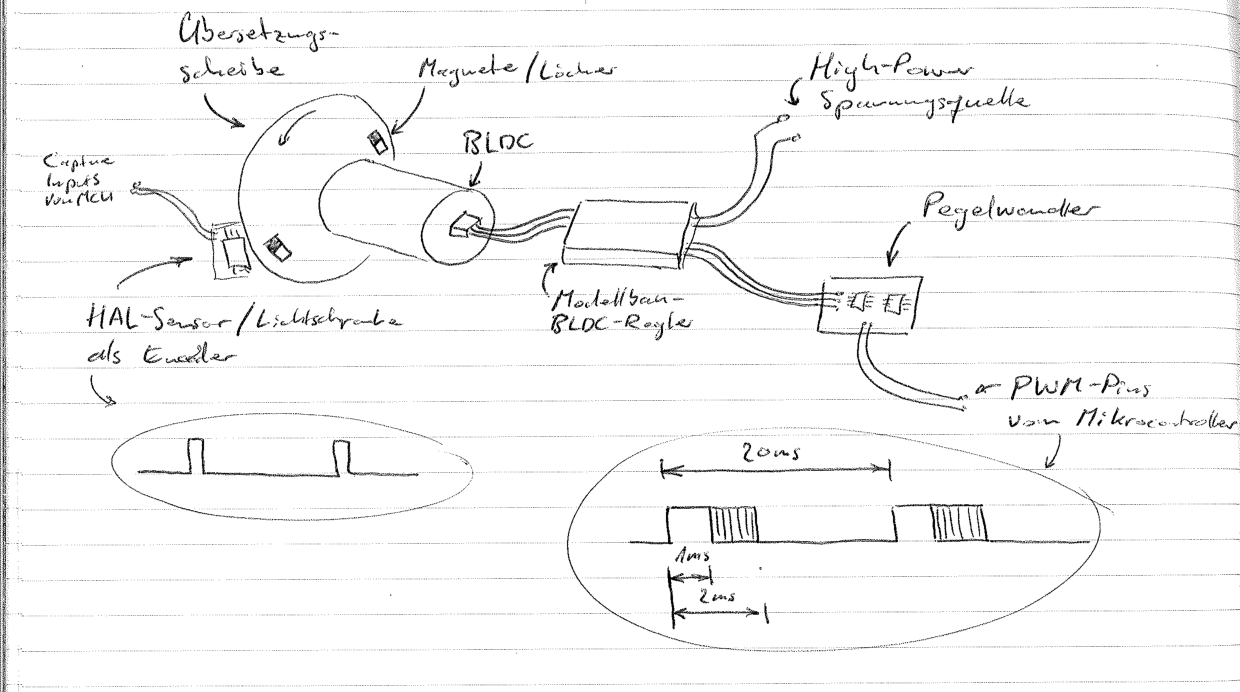
\includegraphics[width=0.8\textwidth]{\EtPath/Bilder/fallback_sketch_1.pdf}
	\caption{Erste Skizze des Fallback-Konzepts}
	\label{fig:fallback-sketch}
\end{figure}
Dieses Feedback wird mittels eines Mikrocontrollers ausgewertet und regelt
damit den Input der Steuerung mit dem PWM-Signal beziehungsweise der Impulsdauer.
Das Einlesen einer Flanke, die Zeitmessung bis zur nächsten Flanke und die
Stellung eines PWM-Signals, sind Tasks welche übliche Mikrocontroller direkt
durch ihre Peripherie-Module ausführen können. Dies ermöglicht eine einfache
Adaption in ein bestehendes Modell, denn es werden lediglich zwei Timer-IO
für diesen Fallback verwendet. Je nach Mikrocontroller ist ein Pegelwandler
für die PWM-Signale notwendig.

    \ifSTANDALONE
\section{Encoder \& Drehzahlgeber}
\fi
\ifEMBED
\subsubsection{Encoder \& Drehzahlgeber}
\fi

Die vorgesehenen Motorfunktionen verlangen lediglich beim Brushlessmotor
nach einem Feedback über die Rotation des Motors, da der Schrittmotor
definiert und fein granuliert betrieben wird. Der Gleichstrommotor stellt
keinerlei Ansprüche, weder an die Drehzahl, noch an die Position.

Encoder sind relativ teuer und der Einsatz des Brushlessmotors verlangt
lediglich nach einem Feedback zur Rotation beziehungsweise Winkelgeschwindigkeit.
Die absolute oder relative Position ist für die Anwendung nicht von
Bedeutung. Somit lässt sich ein einfaches Feedback vorsehen, für die
Regelung der Drehzahl mit optischen oder magnetischen Elementen.
\ifSTANDALONE
\begin{figure}[h!]
	\centering
	\begin{tikzpicture}
	% Koordinaten
	\draw[->] (-0.5, 0) -- (8, 0) node[anchor=north] {$t$};
	\draw[->] (0, -1.5) -- (0, 3) node[anchor=east] {$u,\varphi$};
	% Rotation
	\draw[blue] (0,0) sin (1,1) cos (2,0) sin (3,-1) cos (4,0)
	sin (5,1) cos (6,0) sin (7,-1)
	node[right] {$\varphi$};
	% Signal
	\draw[-, thick, red]
	(0,0) -- (0.8,0) -- (0.8,2) -- (1.2,2) -- (1.2,0) -- 
	(4.8,0) -- (4.8,2) -- (5.2,2) -- (5.2,0) -- (7.5,0);
	% Messung
	\draw[<->] (0.8,1.5) -- (4.8,1.5) node[midway, above] {$t_{r}$};
	\end{tikzpicture}
	\caption{Vereinfachtes Puls-Feedback eines Hall-Effekt-Schalters}
	\label{fig:hall-effekt-schalter}
\end{figure}
\fi
\ifEMBED
\begin{figure}[h!]
	\centering
	\begin{tikzpicture}
	% Koordinaten
	\draw[->] (-0.5, 0) -- (8, 0) node[anchor=north] {$t$};
	\draw[->] (0, -1.5) -- (0, 3) node[anchor=east] {$u,\varphi$};
	% Rotation
	\draw[blue] (0,0) sin (1,1) cos (2,0) sin (3,-1) cos (4,0)
	sin (5,1) cos (6,0) sin (7,-1)
	node[right] {$\varphi$};
	% Signal
	\draw[-, thick, red]
	(0,0) -- (0.8,0) -- (0.8,2) -- (1.2,2) -- (1.2,0) -- 
	(4.8,0) -- (4.8,2) -- (5.2,2) -- (5.2,0) -- (7.5,0);
	% Messung
	\draw[<->] (0.8,1.5) -- (4.8,1.5) node[midway, above] {$t_{r}$};
	\end{tikzpicture}
	\caption{Vereinfachtes Puls-Feedback eines Hall-Effekt-Schalters}
	\label{fig:hall-effekt-schalter}
\end{figure}
\fi
Als optisches Messinstrument kann eine Lichtschranke mit 
Reflexionsstreifen oder Löchern eingesetzt werden. Diese verlangen
nur nach einer geringfügigen Modifikation des rotierenden Körpers und
sind relativ günstig. Optische Messtechnik hat den Nachteil, das
Störungen relativ leicht in die Messung einfliessen können, was fatale
Folgen für die Regelung hat. Magnetische Messinstrumente sind gegenüber
Störungen deutlich resistenter, da hierfür starke Magnetfelder benötigt
werden, welche so nicht einfach auftreten. Der Einsatz einer solchen Messtechnik
verlangt jedoch nach einer Modifikation der Mechanik, da Magnete in den
rotierenden Körper eingebaut werden müssen. Dies birgt ein gewisses
Risiko für mechanische Unwucht des Rotationskörpers.

\ifSTANDALONE
\subsection{Magnetischer Drehzahlgeber}
\fi
\ifEMBED
\paragraph{Magnetischer Drehzahlgeber\\}
\fi
Um einen eigenen magnetischen Drehzahlgeber zu erstellen wird ein
sogenannter Hall-Effekt-Schalter eingesetzt. Dieser reagiert mit seinem Ausgang
auf ein auftretendes Magnetfeld. Das Gegenstück zum Hall-Effekt-Schalter
ist ein Magnet, welcher in das rotierende Objekt eingebaut wird. Aus 
mechanischen Gründen, wie etwa der Unwucht, werden typischerweise 2 Magnete
oder ein Vielfaches davon in den rotierenden Körper eingebaut.

Bei der Rotation des Körpers entstehen durch das Passieren der Magnete
am Hall-Effekt-Schalter Impulse. Aus diesen Impulsen lässt sich mit einer
Zeitmessung direkt die Drehzahl bestimmen. Die Abbildung 
\ref{fig:hall-effekt-schalter} illustriert das Prinzip anhand eines
Beispiels mit einem Magneten am Rotationskörper.
%
\ifSTANDALONE
\begin{figure}[h!]
	\centering
	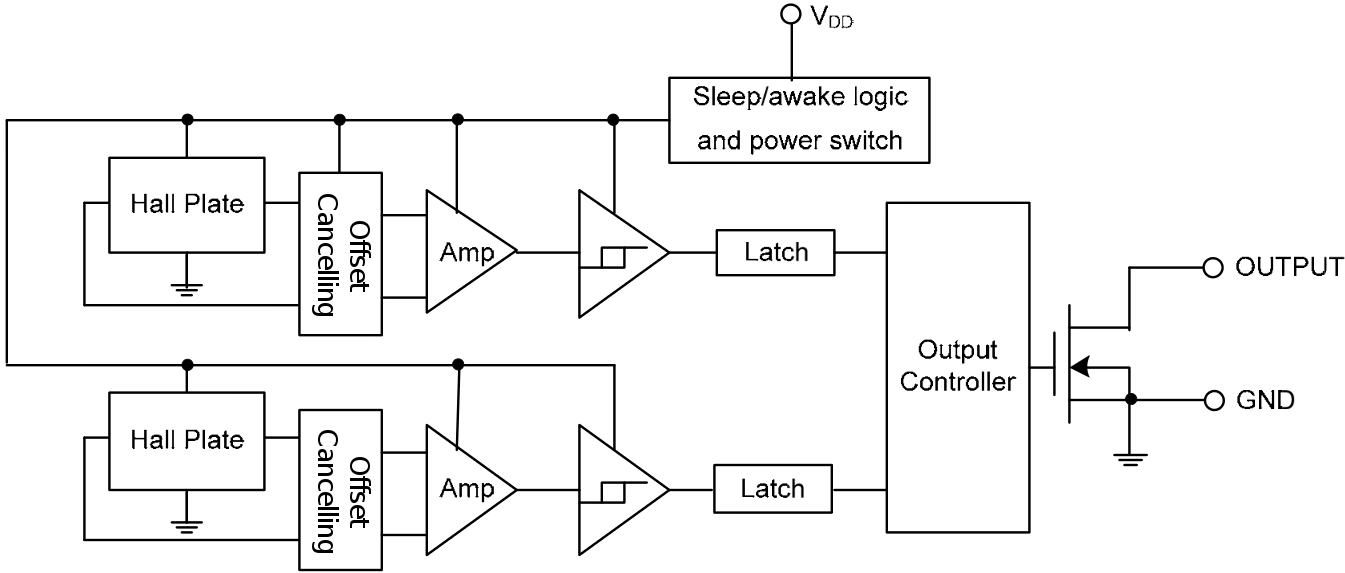
\includegraphics[width=0.75\textwidth]{\EtPath/Bilder/AH180N_functional.png}
	\caption{Funktionelles Blockschaltbild des Hall-Effekt-Schalters AH180N}
	\label{fig:AH180N_functional}
\end{figure}
\fi
%
\ifEMBED
\begin{figure}[h!]
	\centering
	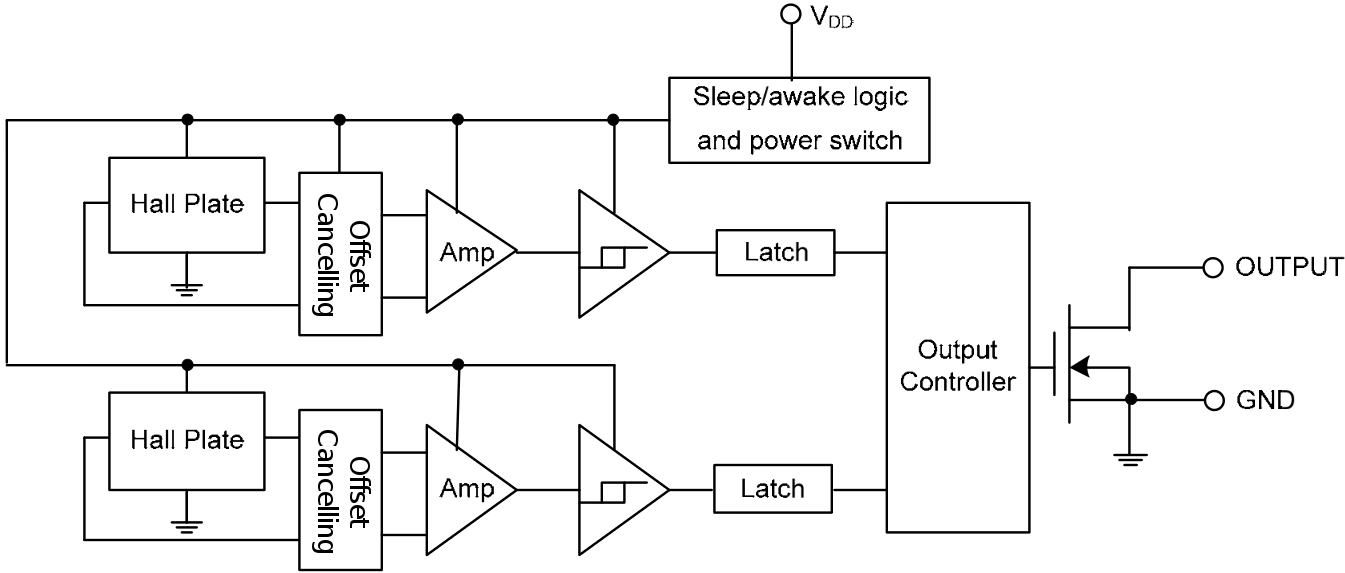
\includegraphics[width=0.75\textwidth]{\EtPath/Bilder/AH180N_functional.png}
	\caption{Funktionelles Blockschaltbild des Hall-Effekt-Schalters AH180N}
	\label{fig:AH180N_functional}
\end{figure}
\fi
%
Ein solches Verfahren lohnt sich bei schnellen Winkelgeschwindigkeiten
und ist für diesen Anwendungsfall sehr effizient. Zugehörige
Hall-Effekt-Schalter lassen sich einfach montieren und sind gegen Störungen
sehr robust. Ein mögliches Modell für einen Hall-Effekt-Schalter ist der
AH180N. Dieser bietet einen Open-Drain Ausgang, welcher somit logische Pegel
liefert (siehe Abbildung \ref{fig:AH180N_functional}). Interessant ist diese
Art von Drehzahl-Geber insbesondere durch ihren geringen Preis, denn solche
Hall-Effekt-Schalter, wie der AH180N, befinden sich im Preissegment von 
unter einem Franken.

    \newpage
    %
    % Projektführung
    %
    \section{Projektplanung /-Management}
	Das Projektteam 32 besteht aus sieben Personen welche sich auf folgende Studienrichtungen aufteilen: 
	Drei Personen aus der Maschinentechnik, drei Personen aus der Informatik und eine Person aus der Elektrotechnik. 
	Die Studienrichtungen sind sogleich die jeweiligen Verantwortungen. In den Bereichen mit mehreren Projektmitgliedern wird die Verantwortung 
	für Teilaufgaben jeweils situativ verteilt. Für allgemeine Projektarbeiten wird je nach Aufgabe eine hauptverantwortliche Person bestimmt. 
	Diese kann Teilaufgaben definieren und sie an andere Teammitglieder zur Bearbeitung delegieren. 
	Die Hierarchie im Team ist bewusst flach und ohne eigentlichen Projektleiter gehalten. 
	Entscheide werden im Plenum diskutiert und gefällt. Die Leitung oder Führung einer Besprechung obliegt dem verantwortlichen Teammitglied  des jeweiligen Themas.
	Mit dieser Teamstruktur ist gewährleistet, dass alle Mitglieder Verantwortung tragen können und müssen. Dies soll die Motivation und die Eigeninitiative fördern.
    \subsection{Kosten}

\begin{figure}[h!]

  \centering
  \caption{Kostentabelle}
    \begin{tabular}{rcrcc}
    \textbf{Kategorie} & \textbf{Stk} & \textbf{Bezeichnung} & \textbf{Preis / Stk} & \textbf{Stk * Preis} \\

    Zuführung: & 1     & Flachbandriemen 	&  Fr. 50.00  &  Fr. 50.00  \\
               & 1     & Achse          	&  Fr. -      &  Fr. -    \\
               & 1     & Welle           	&  Fr. -      &  Fr. -    \\
               & 1     & Zahnrad         	&  Fr. 8.00   &  Fr. 8.00  \\
               & 1     & Zahnrad         	&  Fr. 8.00   &  Fr. 8.00  \\
               & 1     & DC-Motor        	&  Fr. 20.00  &  Fr. 20.00  \\
               &       &                 	&             &  \\
       Geräst: & 2     & Seitenplatte    	&  Fr. 15.00  &  Fr. 30.00  \\
               & 4     & Stützstangen    	&  Fr. -      &  Fr. -    \\
               & 2     & Bodenplättchen  	&  Fr. -      &  Fr. -    \\
               & 1     & Hardware (Controller) &  Fr. 50.00  &  Fr. 50.00  \\
               & 1     & Hardwarekomponenten&  Fr. 40.00  &  Fr. 40.00  \\
               &       &       				&      		  &  \\
Antrieb Schwungräder:  & 2    & Zahnrad Z15 &  Fr. 2.88   &  Fr. 5.76  \\
               & 2     & Zahnrad Z30 		&  Fr.          4.05  &  Fr. 8.10  \\
               & 2     & Zahnrad Z15 		&  Fr.          3.44  &  Fr. 6.88  \\
               & 2     & Zahnrad Z30 		&  Fr.          5.50  &  Fr. 11.00  \\
               & 2     & Welle (Zahnrad - Motor) &  Fr. -    &  Fr. -    \\
               & 2     & Welle (Zahnrad - Zahnrad) &  Fr. -    &  Fr. -    \\
               & 2     & Welle (Zahnrad - Schwungrad) &  Fr. -    &  Fr. -    \\
          & 4     & Kugellager &  Fr. 1.76  &  Fr. 7.04  \\
          & 1     & Schaumstoffband 1m &  Fr. 20.00  &  Fr. 20.00  \\
          & 2     & Schwungrad &  Fr. 20.00  &  Fr. 40.00  \\
          & 2     & Brushlessmotor &  Fr. 34.95  &  Fr.  69.90  \\
          &       &       &       &  \\
    Drehmechanismus: & 1     & Zahnscheibe (Plexiglas) &  Fr. 10.00  &  Fr. 10.00  \\
          & 1     & Zahnrad (Plexiglas) &  Fr. 10.00  &  Fr. 10.00  \\
          & 1     & Servomotor &  Fr. 25.00  &  Fr. 25.00  \\
          & 1     & Bolzen &  Fr. -    &  Fr. -    \\
          & 1     & Gleitlager &  Fr. 5.00  &  Fr. 5.00  \\
          & 1     & Aufnahmeplatte &  Fr.              -    &  Fr. -    \\
          & 1     & Welle &  Fr. -    &  Fr. -    \\
          &       &       &       &  \\
          &       & \textbf{Total:} & \textbf{} & \textbf{ Fr. 424.68 } \\

    \end{tabular}

\end{figure}
    \begin{landscape}
\subsection{Zeit}	
    \begin{figure}[h!]
        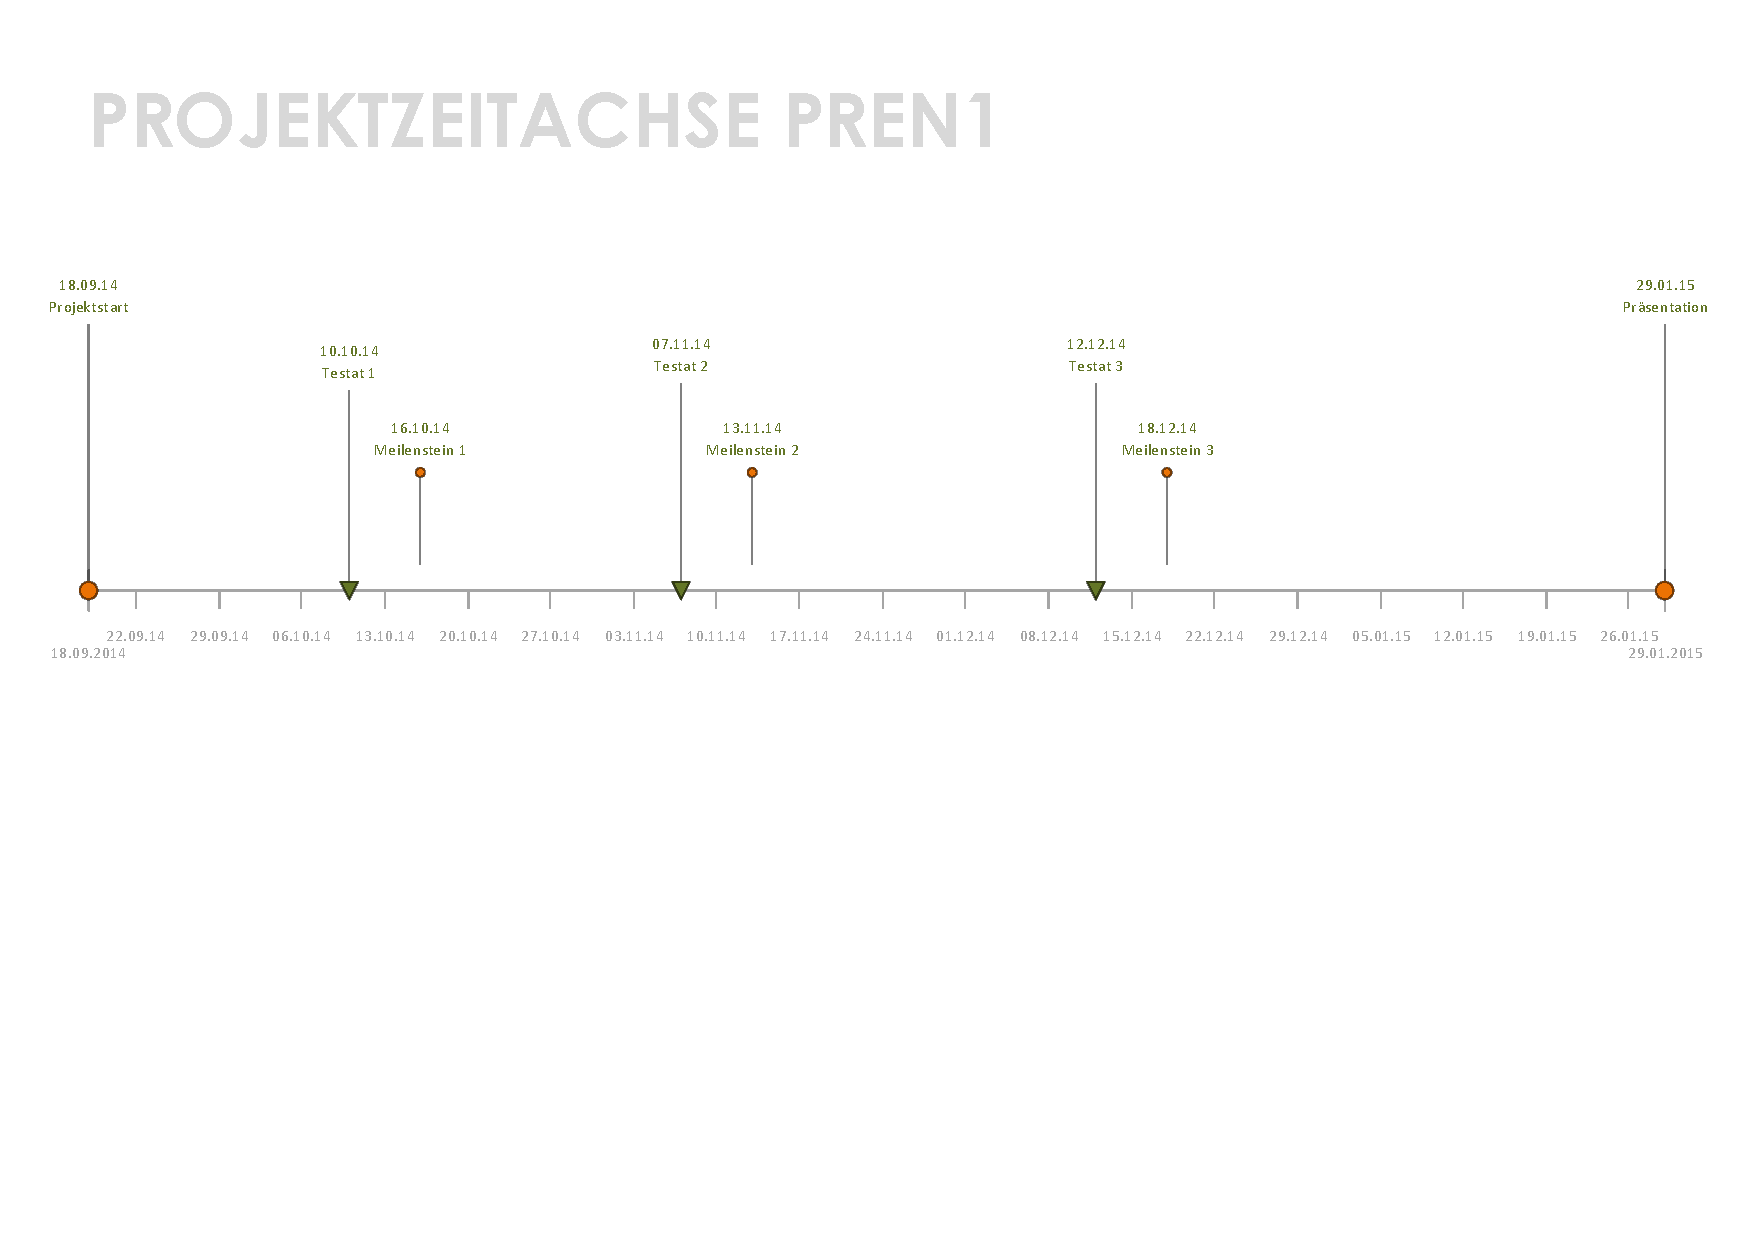
\includegraphics[page=1,scale=0.8,clip,trim=7mm 90mm 31mm 39mm] {Enddokumentation/Projektplanung_Management/Bilder/Projektzeitachse.pdf}
        \centering
        \caption{Zeitplan des Projekts} 
        \label{abb:ProjektZeitstrahl}
    \end{figure}
    
    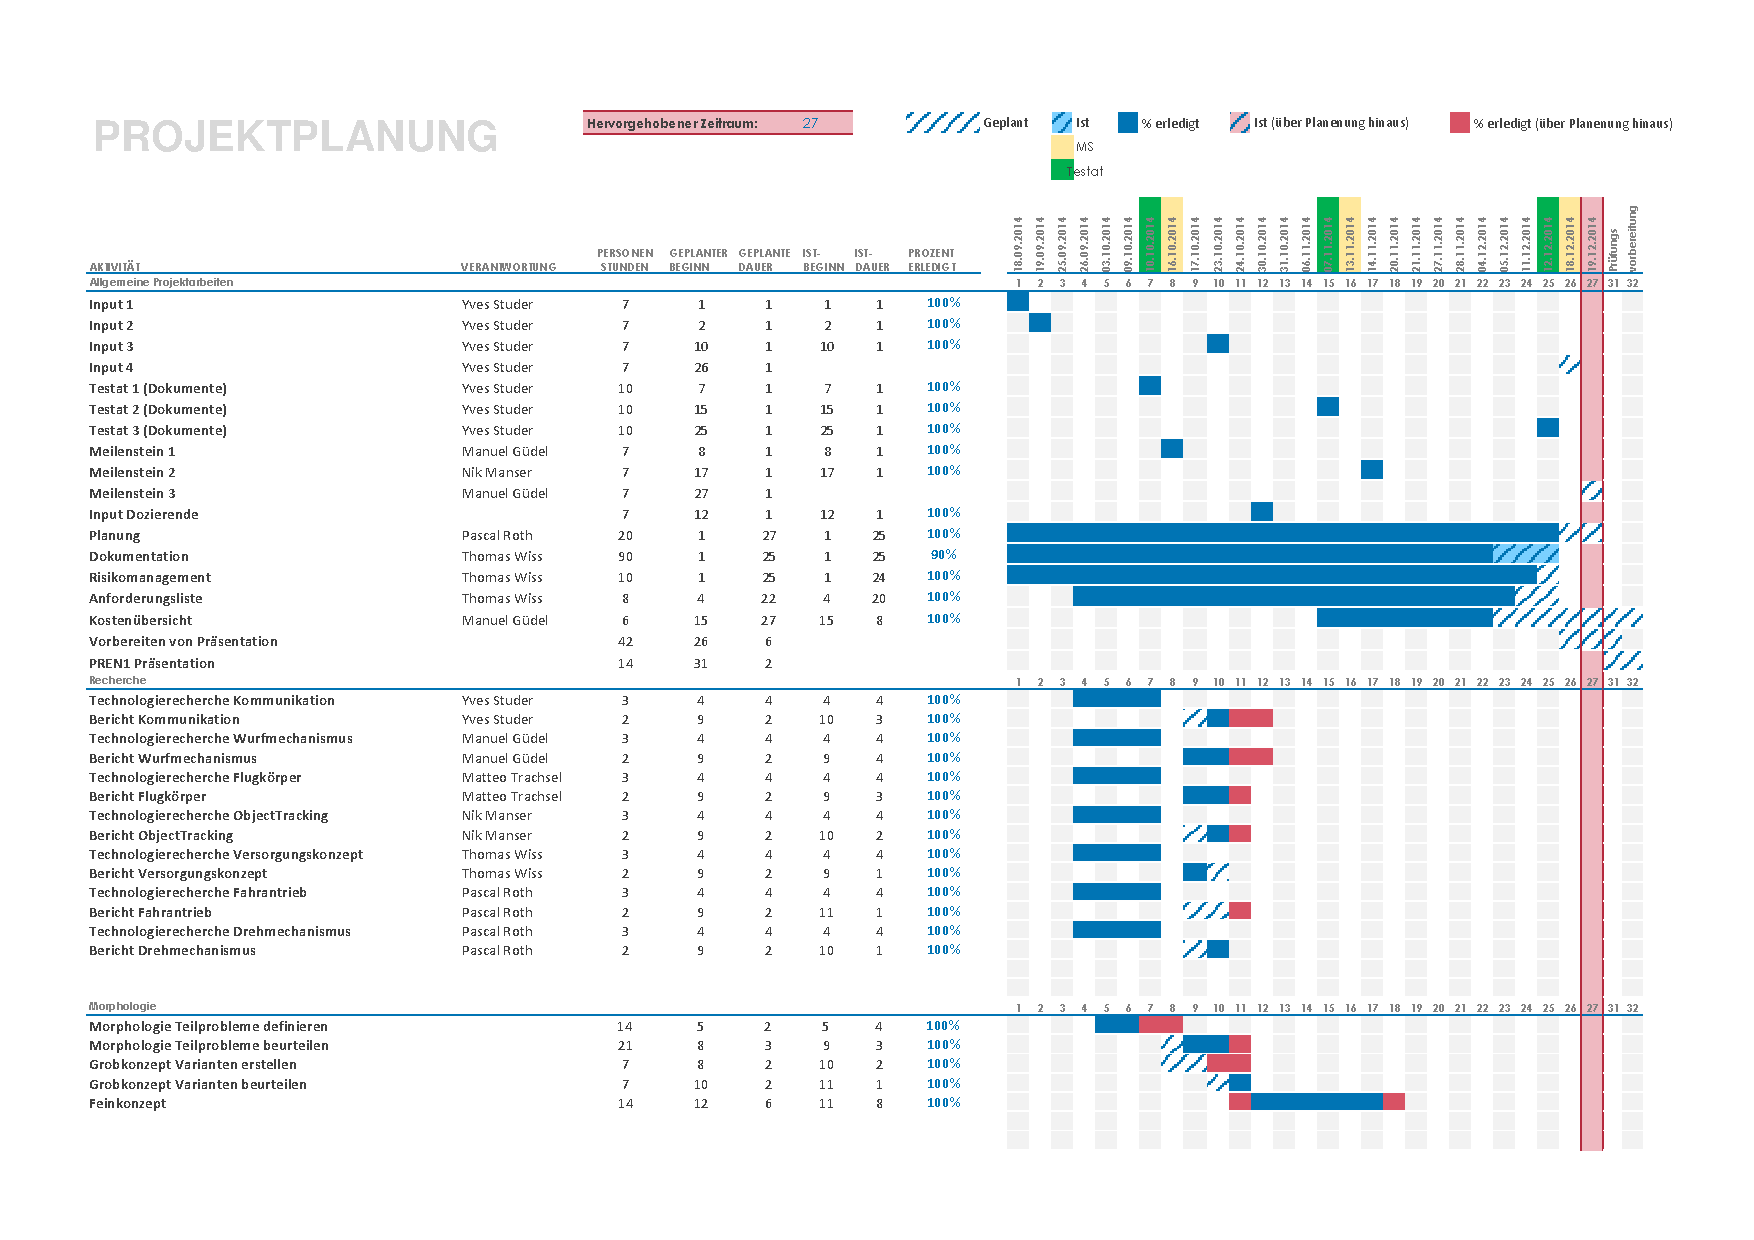
\includegraphics[page=1,scale=0.8,clip,trim=15mm 22mm 13mm 18mm] {Enddokumentation/Projektplanung_Management/Bilder/Projekt-Planung_Team32.pdf}
    \newpage
    \includegraphics[page=2,scale=0.8,clip,trim=15mm 100mm 13mm 10mm] {Enddokumentation/Projektplanung_Management/Bilder/Projekt-Planung_Team32.pdf}
    \newpage
\end{landscape}
\subsubsection{Erläuterung zur Projektplanung}
Um eine grösstmögliche Übersicht zu haben, ist die Projektplanung relativ allgemein gehalten. 
Das heisst, es sind alle Themen und Arbeitsblöcke vorhanden, jedoch ist nicht jeder einzelne Arbeitsschritt der darin anfällt auch aufgeführt. 
Ebenso ist jeweils nur die verantwortliche Person aufgeführt. Sie trägt die Hauptverantwortung über ein Arbeitsblock, 
jedoch können auch andere Personen daran mitgearbeitet haben. Zeitangaben sind als Schätzungen zu verstehen. Es wurde kein Journal über die geleistete Arbeitszeit geführt.\\
Dies ist die Projektplanung über den Zeitraum von PREN1. Arbeiten, die noch nicht fertig sind oder 
die sowieso über den ganzen Zeitraum von PREN laufen, werden Ende PREN1 in eine neue Projektplanung für PREN2 überführt. 
Diese wird mit derselben Excel-Planung gemacht. Dadurch, dass abgeschlossene und nicht mehr relevante Arbeiten nicht mehr aufgeführt sind, wird es wesentlich übersichtlicher.  

    %
    % Reflexion
    %
    \section{Schlussdiskussion}
In einer ersten Phase wurde die Aufgabenstellung in Teilprobleme zerlegt. Für diese partiellen 
Probleme konnte anschliessend nach bestehenden Lösungen recherchiert werden, welche wiederum 
eine Bewertung erhielten und in unterschiedlichen Konstellationen mehrere Grobkonzepte bildeten.\\
\\
Bei der Schaffung der Grobkonzepte mussten einige Grundprobleme angegangen werden. So wurde 
festgelegt, dass ein statischer Werfer konstruiert wird, welcher sich nicht von der Startposition 
wegbewegt. Dies, da sich bei der Verwendung eines Fahrwerks lediglich neue Problemfelder wie 
Rückstoss oder Bestimmung der Eigenposition auftun. Die Verwendung eines Smartphones bot sich 
an, weil dadurch Drahtlos-Adapter, Rechenkapazität und Kamera in einer einzigen Komponente zur Verfügung 
stehen. \\
\\
Dieses grobe erste Konzept wurde weiter ausgearbeitet und daraus ein Feinkonzept geschaffen, 
welches die Grundlage für die Realisierung des Projekts ist: Die Lokalisierung des Korbes wird 
mit einer eigens entwickelten Smartphone-App realisiert. Zum Abwurf der Bälle sollen konkave 
Schwungräder dienen, wobei die Zuführung der Bälle über ein Förderband 
geschieht. \\
\\
Die Elektrotechnik Studierenden haben sich zu einer Gruppe zusammengeschlossen, um 
teamübergreifend gemeinsame Probleme zu lösen. Dies hat sich dahingehend ausgezahlt, dass 
der Brushless Ansteuerungstest mit dem FPGA mit weniger Aufwand als mit einer diskreten Schaltung 
aufgebaut werden konnte. Weiter gibt es Probleme, wie die Stepper-Ansteuerung, die von einer anderen 
Gruppe erarbeitet wird. Ein weiterer wichtiger 
Aspekt dieser Zusammenarbeit ist, dass realitätsnah eine übergeordnete Kollaboration geübt werden 
kann.\\
\\
Insgesamt wurde somit ein Konzept geschaffen, welches die gesetzten Ziele und 
Rahmenbedingungen erfüllt und den sofortigen Beginn der Umsetzung Anfang nächstes Semester 
ermöglicht.
    \subsection{Rückblick}
    \subsection{Ausblick}
Im nächsten Semester wird das erarbeitete Konzept realisiert. Aus administrativer Sicht muss vermehrt und besser zu Beginn einer jeden Meilensteinphase abgesprochen werden, welche Dokumente mit welchem spezifischen Inhalt erstellt werden müssen. Jedes Mal mussten vor einem Meilenstein die Dokumente überarbeitet oder gar neu erstellt werden, weil sich zeigte, dass der Inhalt nicht dem Geforderten entsprach.\\
\\
Mechanisch gesehen steht das Konzept, es fehlen noch einige CAD Zeichnungen, sowie eine geeignete Lösung für den Antriebsstrang der Schwungräder. Des Weiteren muss die Software entwickelt werden. Es wurden bereits Tests zur Bluetooth-Kommunikation, der Objekt erkennung und der Kommunikation zwischen Controller und Smartphone durchgeführt. Diese einzelnen Komponenten müssen jedoch in einer homogenen Smartphone-App integriert werden. Zu Test- und Demonstrationszwecken soll ausserdem der DesktopViewer weiter ausgebaut werden, um Feinabstimmungen über eine GUI-Applikation zu ermöglichen.\\
\\
Ungewissheit besteht ebenfalls betreffend der Mitarbeit von Manuel Güdel. Da er das Modul PREN 2 bereits letztes Jahr absolviert hat, ist noch nicht sicher, ob er nächstes Semester offiziell an der Entwicklung weiterarbeiten kann. Inoffiziell hat er aber bereits seine Hilfe angeboten und wird das Team weiterhin so gut wie möglich unterstützen.

    \newpage
    %
    % Einfügen des Abbildungsverzeichnisses
    %
    \listoffigures 
    %
    % Einfügen des Quellenverzeichnisses mit einem anderen Namen
    %
    \begin{flushleft}
        \renewcommand{\refname}{Literatur- und Quellenverzeichnis}
%        \{\refname}{Quellenverzeichnis}
        \bibliography{Enddokumentation/ET_Gruppe/BLDC_Source,Quellen/Quellen}{} %!!! Kein Leerzeichen nach dem , !!!!
    \end{flushleft}
    %
    % Beginn des Anhangs
    %
    \appendix      
	\begin{appendix}
		\clearpage
		\pagenumbering{Roman} % römische Nummerierung des Anhangs (Grosse Buchstaben)
		\section{Anhang}	            
			\subsection{Berechnung}
\subsubsection{Bestimmung Drehmoment Schwungradantrieb}
\label{BestimmungDrehmomentSchwundrad}
%
Um einen Ball durch die Schwungräder mit einem gewissen Anpressdruck zu führen, wird ein
Drehmoment benötigt. Dazu wird der Tennisball als eine Feder mit der Federkonstante $k$ betrachtet. Zur Ermittlung von $k$ wurde der Ball mit einer Masse $m$ beschwert, und die Verschiebung $x$ gemessen.

\begin{figure}[h!]
	\centering
	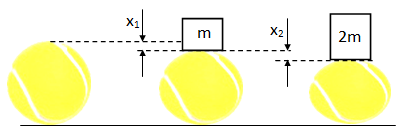
\includegraphics[width=0.6\textwidth]{Enddokumentation/Anhang/Bilder/KompressionBaelle.png}
	\caption{Prinzip der $k$-Bestimmung}
	\label{fig:BallKomp}
\end{figure}

\begin{table}[h!]
	\begin{tabular}{p{1.5cm}p{1.7cm}}
		Gewicht & Auslenkung\\
		\hline
		$1 kg$ & $1 mm$\\
		$2 kg$ & $2 mm$\\
		$3 kg$ & $3 mm$\\
	\end{tabular}
	\centering
	\caption{Resultat der $k$-Bestimmung}
	\label{tab:BallKompErgebnis}
\end{table}

Da $x_1$ und $x_2$ in etwa gleich gross sind, kann von einer linearen Federkonstante
ausgegangen werden. Damit kann die Kraft, die durch das Stauchen des Balles entsteht mit der
Formel
\begin{equation}  
    F_s=2\cdot k \cdot \Delta x 
\end{equation}

bestimmt werden. Die Federkonstante k beträgt $9.8\frac{N}{mm}$ Das entstehende Drehmoment,
wird mit trigonometrischer Beziehung hergeleitet.
\begin{align}  
    \label{equ:Formel_M} %Muss hier sein, damit die Referenz zur ersten Formel zeigt.
    M &= R_S \cdot F_t\\
    F_t &= F_s \cdot \sin(\alpha)\\ 
    F_s &= 2\cdot k \cdot \Delta x 
\end{align}

\begin{figure}[h!]
	\centering
	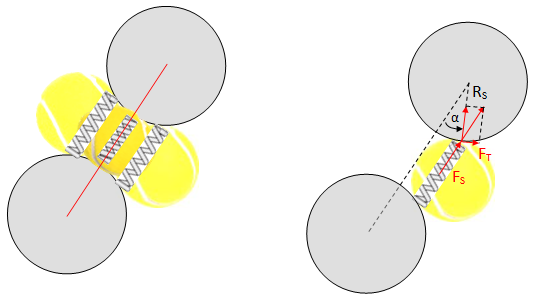
\includegraphics[width=1\textwidth]{Enddokumentation/Anhang/Bilder/PrinzipKompression.png}
	\caption{Prinzip der Kompression}
	\label{fig:PrinzipBallKomp}
\end{figure}

\begin{wrapfigure}{r}{0.3\textwidth}
    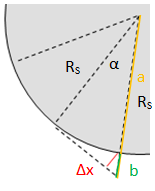
\includegraphics[scale=0.75]{Enddokumentation/Anhang/Bilder/GrafikKreisErkaerung.png}
    \centering
    \caption{keine Ahnung}
    \label{abb:KreisErkaerung}
    \vspace{5mm}
\end{wrapfigure}
Da $\Delta x$ vom Winkel $\alpha$ abhängt, siehe Abbildung \ref{abb:KreisErkaerung} muss die
folgende Abhängigkeit gelten:
\begin{equation}  
	\alpha = R_s \cdot \frac{1}{\cos(\alpha)} \\ \lvert \\ b = a - R_s = R_s \left( \frac{1}{\cos(\alpha)}-1\right)   
\end{equation}

\begin{equation}
	\Delta x = b \cdot \cos(\alpha) = R_a \cdot \left[1 - \cos(\alpha)\right]
\end{equation}

Somit gilt:
\begin{equation} 	\Delta x =  R_s \cdot \left[1 - \cos(\alpha)\right]
	\label{equ:Formel_DeltaX}
\end{equation}

Fügt man nun die Formeln \ref{equ:Formel_M} bis \ref{equ:Formel_DeltaX} zusammen erhält man
das Drehmoment in Abhängigkeit zum Winkel:
\begin{equation}  
    M = 2 \cdot R_s{^{2}} \cdot k \cdot \left[1 - \cos(\alpha)\right] \cdot \sin(\alpha)\\\lvert\\ \left[ |a| \leq \arccos \left(1-\frac{1}{R_s}\right)\right]
\end{equation}
Berechnet mit den Werten $R_s = 40 mm$, $k = 9.8 \frac{N}{mm}$, $L = 146 mm$ und
$DBall = 68 mm$ ergibt sich der folgende Verlauf über den Winkel. Dabei ist ersichtlich,
dass sich das Maximum jeweils beim Grenzwinkel liegt. Dort wird das Drehmoment bei 0 liegen,
da keine Kraft angreift. Der Betrag des maximalen Drehmoments liegt bei $0.174 Nm$ und einem
Winkel von $12.84^\circ$.

\begin{figure}[h!]
	\centering
	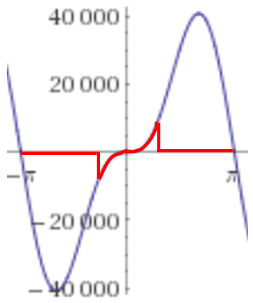
\includegraphics[width=0.3\textwidth]{Enddokumentation/Anhang/Bilder/WeissNicht.png}
	\caption{keine Ahnung}
	\label{fig:keineAhnung}
\end{figure}
Die kurzzeitige Laständerung durch den Abwurf eines Balles kann aufgrund der Trägheit des
Motors nicht ausgeglichen werden. Deshalb soll eine Energiebilanz Aufschlüsse über den
Drehzahlverlust geben. Der Ball hat zwischen den Punkten 0 und 1 zwei verschiedene Energien.
Eine potentielle sowie eine kinetische Energie. Zusätzlich besitzen die Schwungräder
aufgrund ihrer Trägheit eine Rotationsenergie.
\begin{align}
 	&\sum E_{pot} &+&& \sum E_{kin} &&+&& \sum E_{rot} &= 0 \\
 	& m_{ball} \cdot \left(h_1 - h_0\right) &+&&\frac{1}{2} \cdot \left( v_1{^{2}} - v_0{^{2}} \right) &&+&&\frac{1}{2} \cdot J \left( \omega_1{^{2}} - \omega_0{^{2}} \right) &= 0
\end{align}

Die Berechnung der Anfangsgeschwindigkeit des Balles ist von der Zuführgeschwindigkeit wie
folgt abhängig:
\begin{equation}
 	v_0 = v_{band} \cdot \cos(\beta)
\end{equation}

Die Endgeschwindigkeit kommt aufgrund des schiefen Wurfes zustande
\begin{figure}[h!]
	\centering
	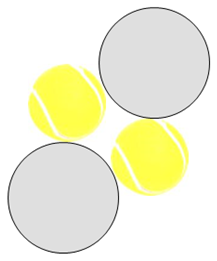
\includegraphics[width=0.3\textwidth]{Enddokumentation/Anhang/Bilder/Ballnachfuehrung.png}
	\caption{keine Ahnung}
	\label{fig:Ballnachführung}
\end{figure}

Das Trägheitsmoment beträgt
\begin{equation}
 	J = \sum_{i}^{N} m_ir_i{^{2}}
\end{equation}

Somit ist eine grosse Masse in weitem Abstand zur Achse anzustreben. Es wird das Trägheitsmoment eines Vollzylinders für die Berechnung verwendet. Dieser lautet:
\begin{equation}
 	J = \frac{1}{2} m \cdot r^2
\end{equation}

Die Masse ist dabei 	
\begin{equation}
	m = \rho \cdot V \\\lvert\\ m = \rho \cdot d_{rad} \cdot \pi \cdot b_{rad}
\end{equation}
Das resultierende Trägheitsmoment beträgt $0.00018 kg m^2$\\
\\
\begin{wrapfigure}{r}{0.3\textwidth}
	 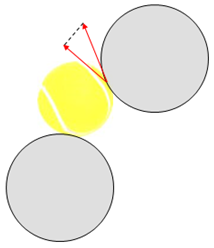
\includegraphics[scale=0.75]{Enddokumentation/Anhang/Bilder/AbwurfBild.png}
	 \centering
	 \caption{keine Ahnung}
	 \label{abb:AbwurfBild}
\end{wrapfigure}
Zwischen der Abwurfgeschwindigkeit und der Winkelgeschwindigkeit gibt es eine Relation.
Dabei wird angenommen, dass der Ball ohne Schlupf die Schwungräder durchläuft. Im
Eintrittspunkt wird der Ball mit einem Sprung beschleunigt. Beim Winkel alpha=0 ist die
Geschwindigkeit am höchsten. Danach wird der Ball wieder abgebremst.
\begin{align}
	v_1 &= v_u \cdot \cos(\alpha)\\
	v_u &= 4\pi \cdot R_s \cdot n_1
\end{align}

Der Höhenunterschied $\delta H$ wird ausgedrückt durch:
\begin{equation}
	\Delta H = \frac{L \cdot \tan(\alpha)}{\sqrt{2}}
\end{equation}

Die Winkelgeschwindigkeiten werden durch die Drehzahl definiert:
\begin{equation}
	\omega = 2\pi \cdot n
\end{equation}

Nun kann die Energiegleichung aufgestellt werden:
\begin{multline}
	m_{Ball} \cdot g \cdot \frac{L \cdot \tan(\alpha)}{\sqrt{2}} + \frac{1}{2} \cdot m_{Ball} \cdot \left(\left[4\pi \cdot R_s \cdot n_1 \cdot \cos(\alpha)\right]^2 - \left[ v_{Band} \cdot \frac{1}{\sqrt{2}}\right]^2\right) +\\
	\frac{1}{2} \cdot J \cdot \left(\left[2\pi \cdot n_1\right]^2 - \left[2\pi \cdot n_0\right]^2\right) = 0
	\label{equ:AbbremsungBall}
\end{multline}
Berechnet mit den gegebenen Werten von: $mBall = 0.055 kg$, $g = 9.81\frac{N}{kg}$, $L = 0.146 m$, $R_s = 0.040 m$, $v_{Band} = 0 \frac{m}{s}$, $J = 0.00018 kgm^2$, $n_0 = 41\frac{U}{s}$, $a = 12.84^\cdot$ ergebt sich eine Drehzahl von $24.2 \frac{U}{s}$. Dies entspricht 58\% der Nenndrehzahl.\\
\\
Verdoppelt man nun das Trägheitsmoment J, so steigt die Nenndrehzahl auf $29.6 \frac{U}{s}$
an. Dies entspricht 71\% der Nenndrehzahl.\\
\\
Als nächstes wird die Zeit für das Beschleunigen der Räder von der abgebremsten Drehzahl
wieder auf die Nenndrehzahl berechnet.
\begin{align}
	M &= \alpha \cdot J\\
	n_0 &= n_1 + \alpha \cdot t
\end{align}
Somit gilt:
\begin{equation}
	t = \frac{n_0 - n_1}{\alpha} = \frac{\Delta n \cdot J}{M}
\end{equation}
Wir setzen nun vereinfacht, für das Trägheitsmoment, dieses des Schwungrades ein. Das Moment
des Motors soll $0.5 Nm$ betragen. Somit resultiert ein t von $6 ms$. 

Um die Abwurfgeschwindigkeit des Balles aus dem Wurfgerät zu bestimmen, wurde der schiefe
Wurf ohne Luftwiderstand berechnet, da für diese Anwendung die Abweichung durch den
Luftwiderstand minimal ist.
\begin{figure}[h!]
	\centering
	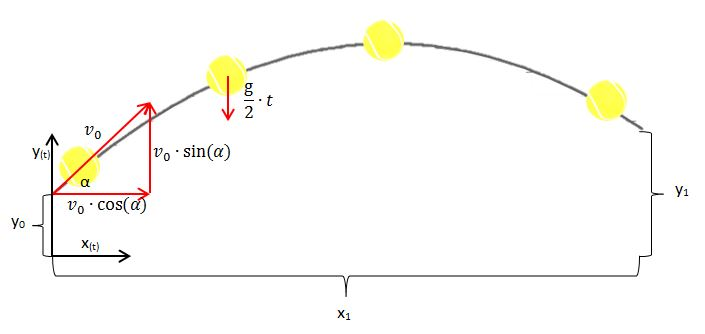
\includegraphics[width=0.9\textwidth]{Enddokumentation/Anhang/Bilder/Schiefer_Wurf2.jpg}
	\caption{Wurfparabel}
	\label{fig:Wurfparabel}
\end{figure}
\begin{align}
	x_{(t)} &= v_0 \cdot \cos(\alpha_0)\\
	y_{(t)} &= y_0 + v_0 \cdot t \cdot \sin(\alpha_0) - \frac{1}{2} \cdot g \cdot t^2
\end{align}

Mit den definierten Werten $x_1 = 1.8 m$, $y_0 = 0.125 m$, $y_1 = 0.4 m$ und 
$g = 9.81 \frac{m}{s}$ ergibt sich eine Zeitdauer von $t = 0.56 s$ und eine
Abwurfgeschwindigkeit von $4.56 \frac{m}{s}$ Die nachfolgende Abbildung
\ref{fig:Wurfparabel1} zeigt die resultierende Wurfparabel.
\begin{figure}[h!]
	\centering
	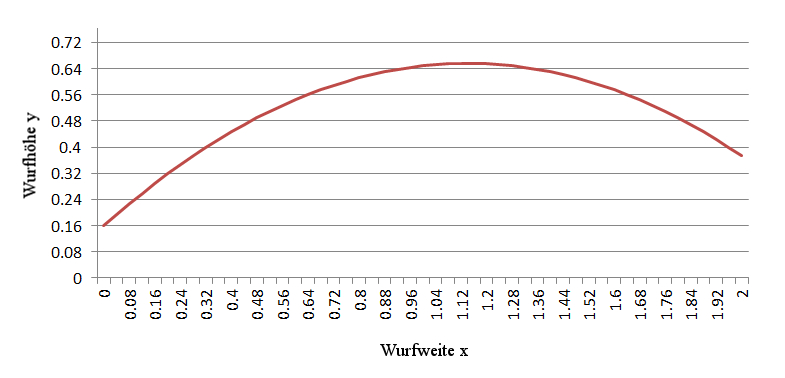
\includegraphics[width=1\textwidth]{Enddokumentation/Anhang/Bilder/Schiefer_Wurf.jpg}
	\caption{Wurfparabel}
	\label{fig:Wurfparabel1}
\end{figure}

\textbf{Berechnung des Drehmoment des Förderbands}\\
%\begin{figure}[h!]
%	\centering
%	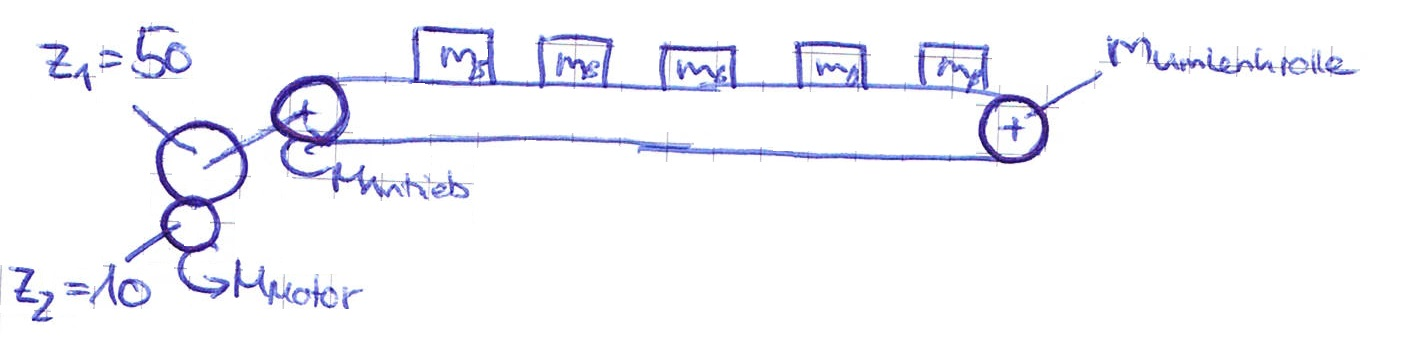
\includegraphics[width=1\textwidth]{Enddokumentation/Anhang/Bilder/FoerderbandSkizze.jpg}
%	\caption{Erläuterungen zur Förderbandberechnung}
%\end{figure}\\

\begin{figure}[h!]
    \begin{tikzpicture}[scale = 1.2]
    \draw [-,line width=2pt](0,0) circle (10pt);\draw [-,line width=2pt](6,0) circle (10pt); %beide Kreise der hauptrollen
    \draw  (0,10pt) -- (6, 10pt); \draw (0,-11pt) -- (6,-11pt); %die beiden Förderbänder-Striche
    \draw (0,-2pt) -- (0, 2pt); \draw (0cm-2pt,0) -- (0cm+2pt, 0); %Das x der ersten Rolle
    \draw (6,-2pt) -- (6, 2pt); \draw (6cm-2pt,0) -- (6cm+2pt, 0); %Das x der zweiten Rolle
    \draw [<-] (6cm-0pt , 5pt) -- (7,0.5)node[right]{$m_{Umlenkrolle}$}; %zeige-Linie auf das Hintere Rad mit Text
    \draw (5,10pt) -- (5, 24pt);\draw (5.7,10pt) -- (5.7, 24pt);\draw (5,24pt) -- (5.7, 24pt);\node  at (5.35,18pt) {$m_B$};
    \draw (3.875,10pt) -- (3.875, 24pt);\draw (4.575,10pt) -- (4.575, 24pt);\draw (3.875,24pt) -- (4.575, 24pt);\node  at (4.2,18pt) {$m_B$};
    \draw (2.75,10pt) -- (2.75, 24pt);\draw (3.45,10pt) -- (3.45, 24pt);\draw (2.75,24pt) -- (3.45, 24pt);\node  at (3.1,18pt) {$m_B$};
    \draw (1.625,10pt) -- (1.625, 24pt);\draw (2.325,10pt) -- (2.325, 24pt);\draw (1.625,24pt) -- (2.325, 24pt);\node  at (1.975,18pt) {$m_B$};
    \draw (0.5,10pt) -- (0.5, 24pt);\draw (1.2,10pt) -- (1.2, 24pt);\draw (0.5,24pt) -- (1.2, 24pt);\node  at (.8,18pt) {$m_B$};
    \draw (0,-18pt) circle (7pt);  \draw [<-] (2pt , -20pt) -- (25pt,-25pt)node[right]{$m_{Antrieb}$}; %zeige-Linie auf das Antriebsrad mit Beschriftung
    \draw [<-] (-4pt , 4pt) -- (4pt,1.3)node[right]{$z_1 = 50$}; %zeige-Linie auf das linke Umlenkrad mit Beschriftung
    \draw [<-] (-3pt , -19pt) -- (4pt,-1.6)node[right]{$z_2 = 10$}; %zeige-Linie auf das Antriebsrad mit Beschriftung
    \end{tikzpicture}
   	\centering
    \caption{Erläuterungen zur Förderbandberechnung}
\end{figure}
Formalismus:
\begin{align}
    \label{equ:DrehmomentFörderband}
    M_{Motor} &= M_{Antrieb} \cdot i\\
    i &=\frac{z_1}{z_2}\\
    M_{Antrieb} &= F_u \cdot r_A\\
    F_u &= \mu_T \cdot g \cdot \left(5 \cdot m_B + m_{Umlenkrolle} + m_{Band} \right)\\
    M_{Motor} &= \mu \cdot g \cdot r_A \cdot \left(5 \cdot m_B + m_{Umlenkrolle} + m_{Band}\right) \cdot \frac{z_1}{z_2}
\end{align}
Verwendete Werte:\\
$\mu_T = 0.33$\\
$g = 9.81\frac{m}{s^2}$\\
$r_A = 0.008 m$\\
$m_B = 0.055 kg$\\
$m_{Umlenkrolle} = 0.020 kg$\\
$m_{Band} = 0.035 kg$\\
$z_1 = 50$\\
$z_2 = 10$\\
Daraus ergibt sich ein Drehmoment von $0.0017 Nm$ = \uuline{$1.7 Nmm$}\\
\\
\textbf{Berechnung Drehmoment des Ausrichtungsmechanismus}\\
\begin{wrapfigure}{r}{0.43\textwidth}
	\centering
	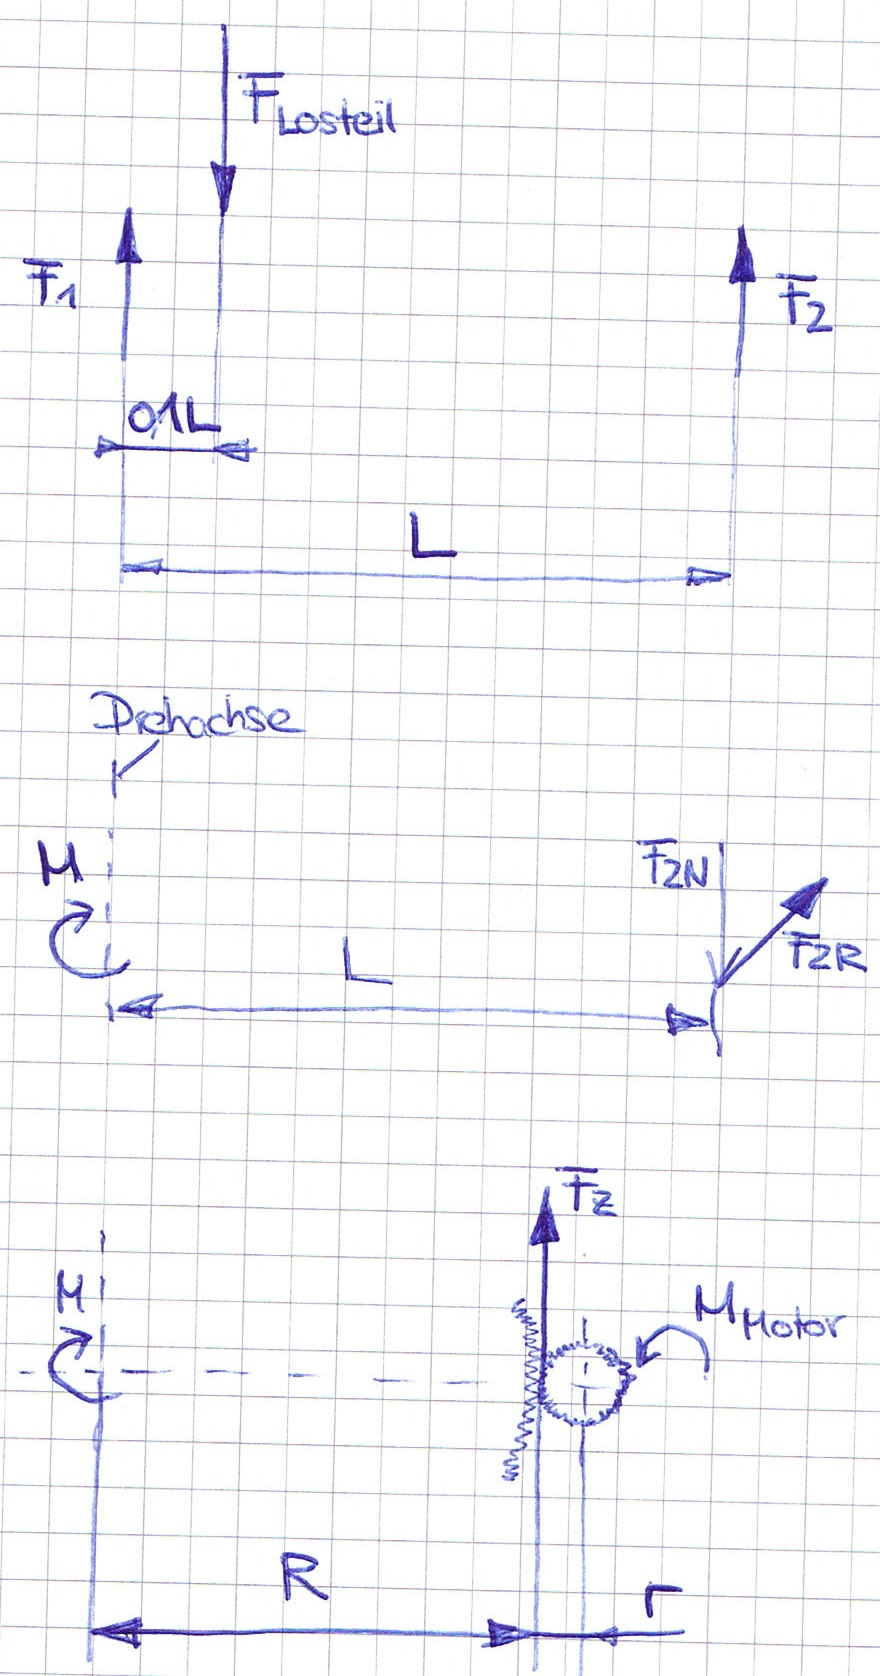
\includegraphics[width=0.45\textwidth]{Enddokumentation/Anhang/Bilder/NotizBerechnungDrehmomentStepper.jpg}
	\caption{Erläuterungen zur Schrittmotorberechnung}	
\end{wrapfigure}
Formalismus:
\begin{align}
    F_{Losteil} &= m_{Losteil} \cdot g\\
    F_2 &= F_{Losteil} \cdot 0.1
\end{align}

\begin{align}
    M_{Drehung} &= L \cdot F_{2R}\\
    F_{2R} &= \mu_H \cdot F_2
\end{align}

\begin{align}
    M_{Motor} &= F_z \cdot r\\
    F_z &= \frac{M_{Drehung}}{R}\\
    M_{Motor} &=\frac{L \cdot \mu_H \cdot m_{Losteil} \cdot g \cdot 0.1}{R} \cdot r
\end{align}
Verwendete Werte:\\
$L = 0.437m$\\
$\mu_H = 0.2$\\
$m_{Losteil} = 1.6 kg$\\
$g = 9.81 \frac{m}{s^2}$\\
$R = 0.28 m$\\
$r = 0.01 m$\\
Daraus ergibt sich ein Drehmoment von \\
$0.0049 Nm$ = \uuline{$4.9 Nmm$}\\

			
\includepdf[page=1 , offset=0cm 0cm,frame, width=\textwidth,picturecommand={\centering},pagecommand=\subsection{Stepper-Dokumentation}\label{Stepper_Dokumentation}{\thispagestyle{fancy}},]{Enddokumentation/Anhang/Extern/Stepper_StandaloneDoc.pdf}

%pagecommand=\section{Projektplan}
\includepdf[page=2- , offset=0cm 0cm,frame, width=\textwidth,picturecommand={\centering},pagecommand={\thispagestyle{fancy}},]{Enddokumentation/Anhang/Extern/Stepper_StandaloneDoc.pdf}
	\end{appendix}  
\end{document}